%************************************************
\chapter{Results}\label{ch:results} % $\mathbb{ZNR}$
%************************************************
Decentralized \acs{STG} preparations have descending modulatory inputs from the \acsp{CoG} and \acs{OG} removed. \acs{STG} neurons in a decentralized state exhibit a slower burst frequency and variable network activity\autocite{HamoodAnimaltoanimalvariabilityneuromodulation2014, HamoodConsequencesacutelongterm2015}. This effect can be restored to normal function by exogenous application of modulatory substances into the saline bath\autocite{SwensenModulatorsconvergentcellular2001, SharpDynamicclampcomputergenerated1993}. Proctolin and \acs{RPCH} are neuromodulators which open a mixed cation inward modulatory input current \ac{IMI}\autocite{SwensenModulatorsconvergentcellular2001}. 

To model decentralization and modulation, single-neuron \ac{AB} models and network (\acs{AB}-\acs{PD}, \acs{LP}, \acs{PY}) models were constructed according to the Hodgkin-Huxley formalism\autocite{PrinzAlternativehandtuningconductancebased2003, PrinzSimilarnetworkactivity2004, HodgkinMeasurementcurrentvoltagerelations1952, Hodgkincomponentsmembraneconductance1952, Hodgkinquantitativedescriptionmembrane1952}. Maximal conductances were determined by particle swarm optimization (\autoref{sec:parameteroptimization}) to respond to modulatory input in the form of \acs{IMI}\autocite{SwensenModulatorsconvergentcellular2001}. \acs{AB} and the two \acs{PD} cells were combined into a computational composite \acs{AB}-\acs{PD} since the cells are strongly electrically coupled (\autoref{fig:prinz1}). Similarly, electrically-coupled \acs{PY} cells were combined into a single computational composite, following \citeauthor{PrinzSimilarnetworkactivity2004}\autocite{PrinzSimilarnetworkactivity2004} The \acs{AB}-\acs{PD} pacemaker kernel synapses onto \acs{LP} and \acs{PY} with inhibitory glutamatergic and cholinergic synapses. \acs{LP} and \acs{PY} reciprocally inhibit each other and \acs{LP} feeds back onto the pacemaker kernel (\autoref{fig:pyloricrhythm}).

\acs{AB} increases in frequency and amplitude from baseline in bath-applied proctolin\autocite{SharpDynamicclampcomputergenerated1993, SwensenMultiplepeptidesconverge2000, SwensenModulatorsconvergentcellular2001, GolowaschProctolinactivatesinward1992}. Modulatory input conductance (\autoref{sec:modulatoryinput}) was added to single-compartment models from the Prinz database\autocite{PrinzAlternativehandtuningconductancebased2003} to characterize the effect of \acs{IMI} on a population of previously studied models. Most models did not respond to \acs{IMI}, so maximal conductances were manipulated in a particle swarm optimization protocol to produce models which increase in frequency and amplitude to increasing \acs{IMI} maximal conductance\autocite{NusbaumNeuronalRoleCrustacean1988,SharpDynamicclampcomputergenerated1993}.

\acs{RPCH} activates a modulatory input conductance in \acs{AB} and \acs{LP} cells. Network models were simulated under \acs{IMI} conductance in \acs{AB}-\acs{PD}, \acs{LP} and both model neurons to simulate neuromodulation by \acs{RPCH}. Maximal conductances of the three model neurons and synapses were manipulated by particle swarm optimization to produce models with slow, unstable rhythms in the decentralized condition and increased burst frequency and amplitude under neuromodulation. While modulation onto the pacemaker and \acs{LP} recapitulated experimental findings (\autoref{fig:rosenbaum2}), modulation into \acs{AB}-\acs{PD} and \acs{LP} produced the most stable rhythms. 

\section{Modulation in AB Models Switches Between Amplitude States}
To develop an initial set of solutions to optimize (the ``seed''), neurons from the \acs{STG} neuron database were simulated\autocite{PrinzAlternativehandtuningconductancebased2003}. This database contains ~2.2 million model neurons with linearly spaced parameters. Neurons flagged as ``bursting neurons'' were simulated with increasing levels of modulatory input. Since \acs{AB} does not fire strong action potentials (\autoref{fig:sharp2}) and responds to \acs{RPCH} under the potent sodium channel blocker \acs{TTX}, \ac{INa} and \acs{ICaT} maximal conductances set to zero to eliminate sodium and calcium spikes respectively\autocite{NusbaumNeuronalRoleCrustacean1988}. These models would serve as a testbed for exploring neuromodulation in isolated cells.

Quiescent models were defined as having amplitude < 20 mV to isolate models that appear similar to decentralized preparations in \ac{TTX}\autocite{NusbaumNeuronalRoleCrustacean1988}. Slow wave amplitude was defined as the maximal peak voltage minus the minimal trough voltage at steady-state ($10~\mathrm{s} < t < 20~\mathrm{s}$).

Modulatory input was applied to these low-amplitude oscillators ($n = 14,700$), which were simulated for 20 s (\autoref{fig:prinzburstingmodelsnavcatswensen}). The first 10 s were discarded as transient and burst frequency and amplitude were computed. To test sensitivity to initial conditions, the simulations were repeated with $V_m = 60$ mV and $m_{MI} = 1$ instead of standard initial conditions (\autoref{tab:initialconditions}). No significant differences were observed.

\begin{figure}[h]
	\centering
	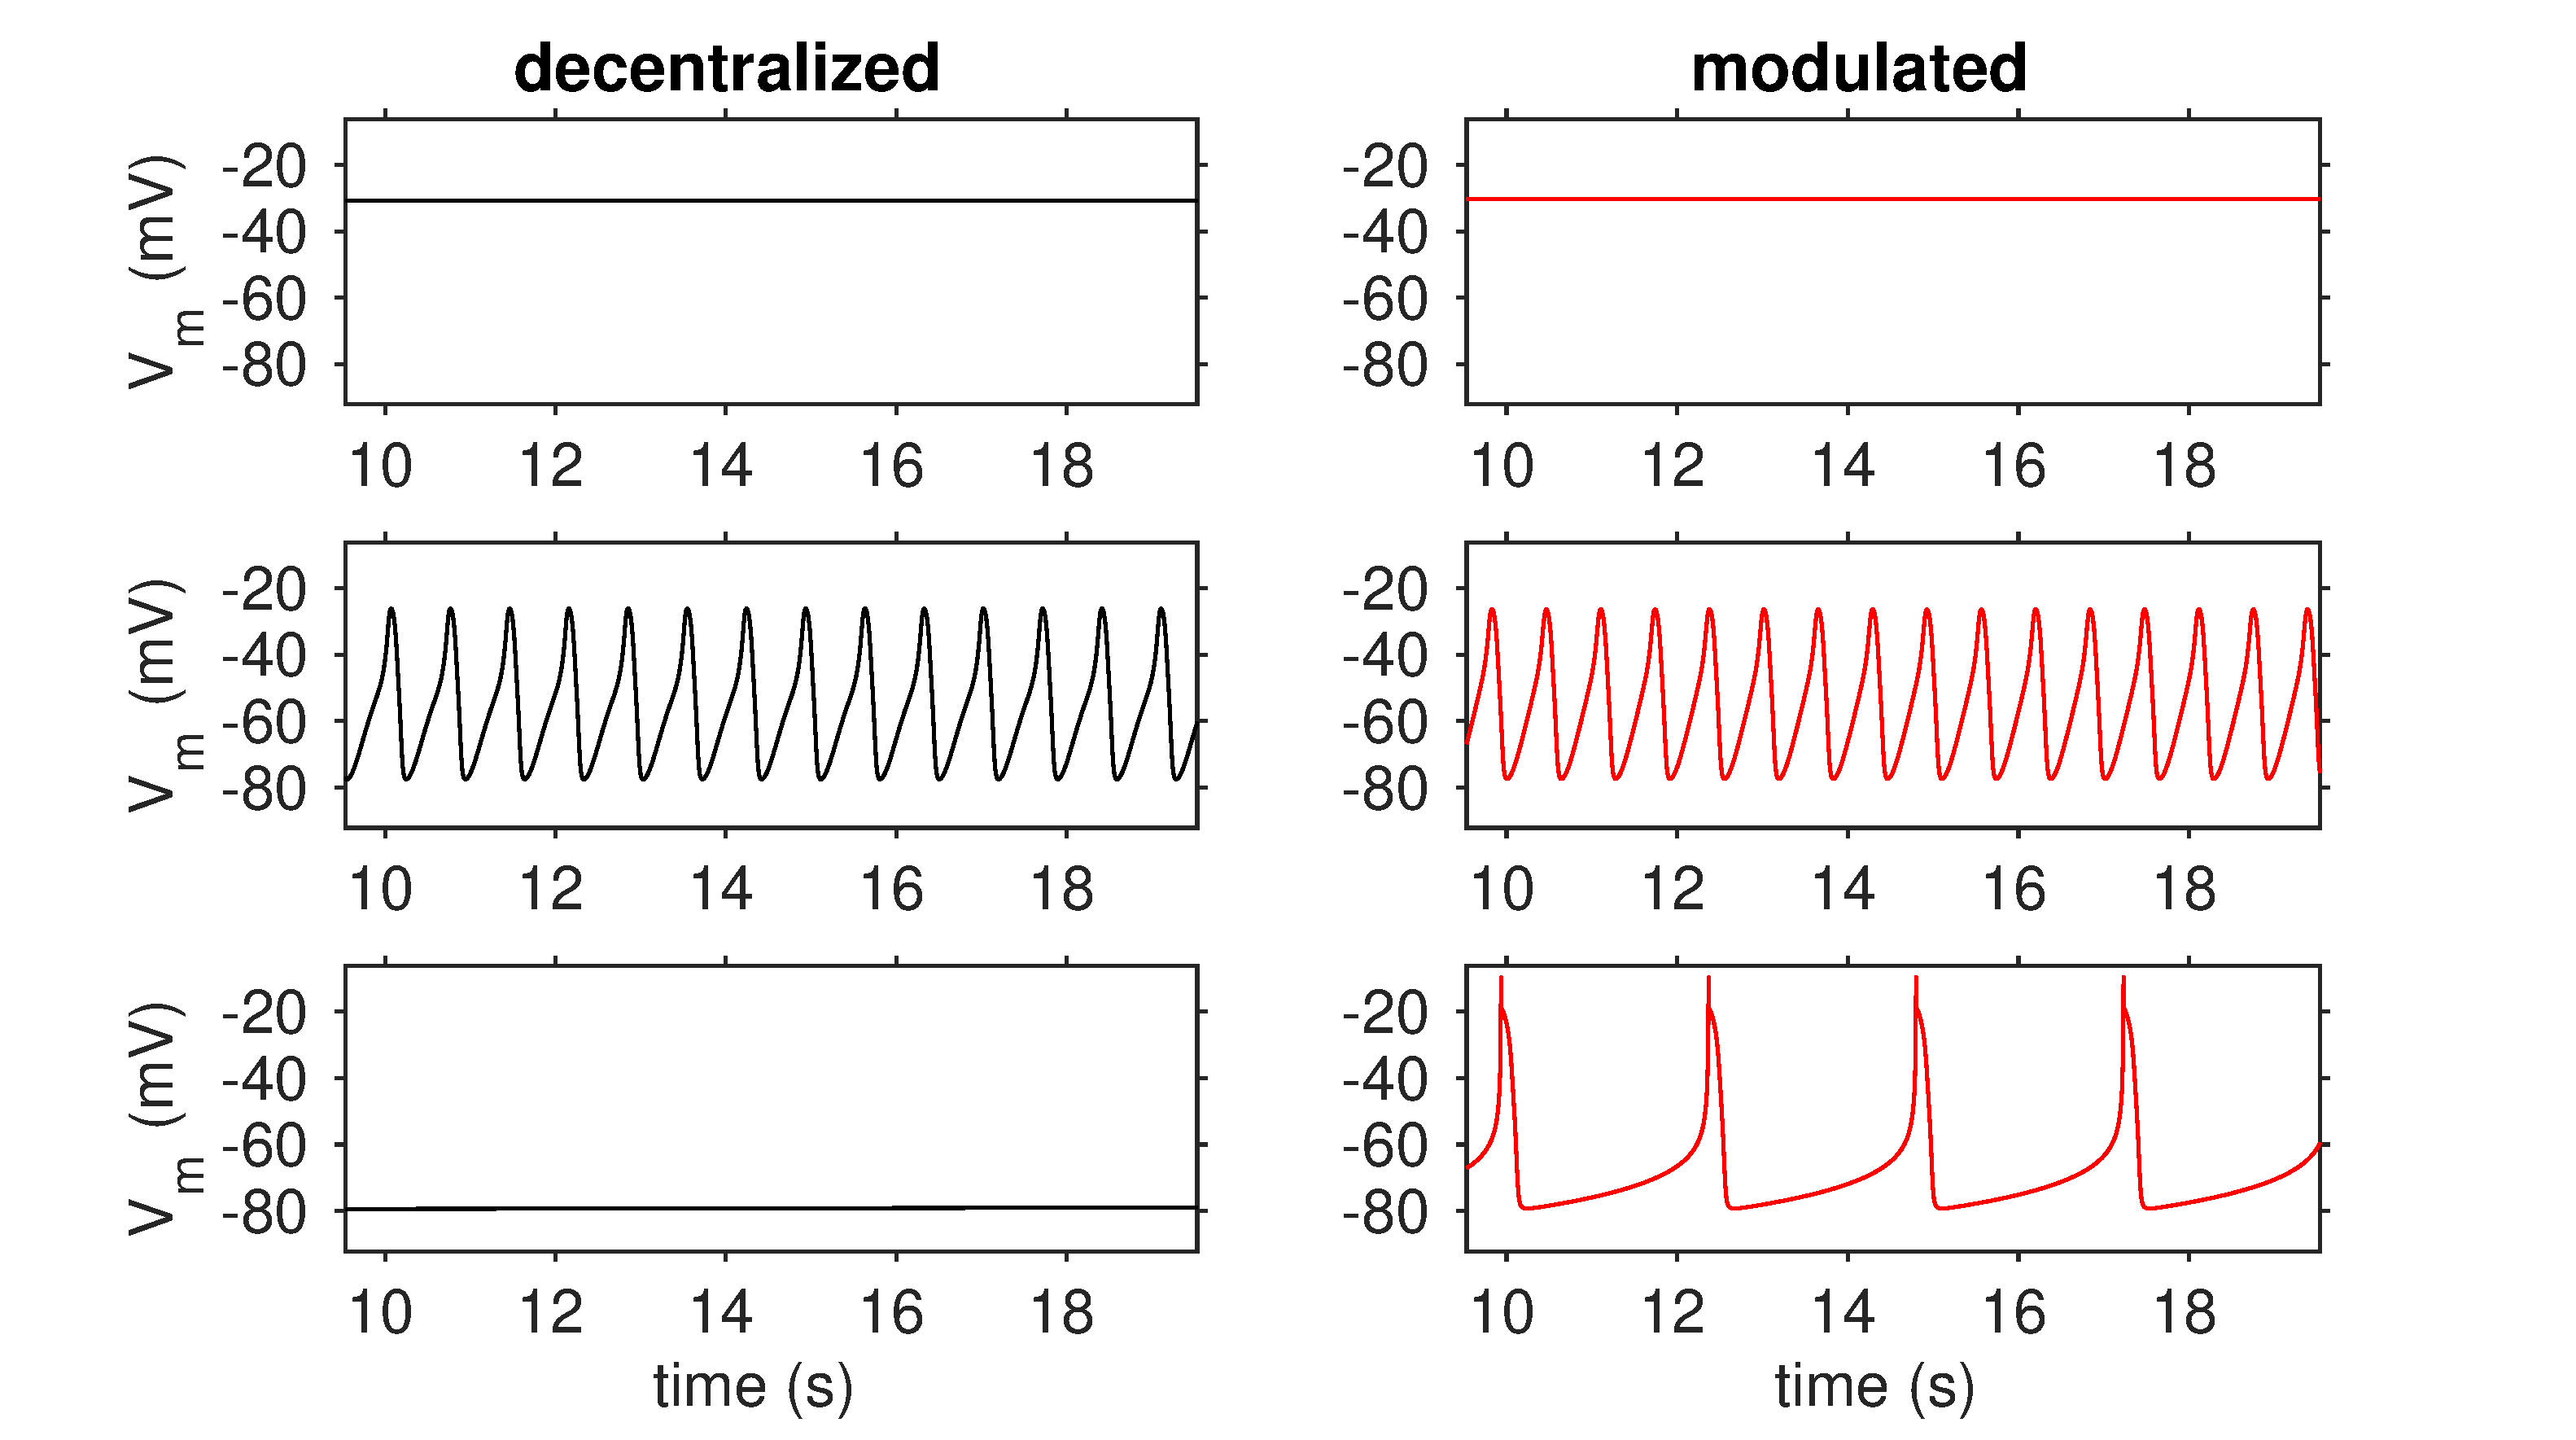
\includegraphics[width=1.0\linewidth]{gfx/prinz-models/tracePrinz}
	\caption[Three motifs of modulation in model AB neurons]{Three motifs of modulation in model \acs{AB} neurons from the \acs{STG} database.  Most model neurons from the Prinz \acs{STG} database without \acs{INa} or \acs{ICaT} conductance remained quiescent. A subset of models oscillated in both conditions and < 100 switched from quiescence to oscillation. Black traces demonstrate the non-modulated case and red traces indicate $\bar{g}_MI = 1~\mu \mathrm{S/mm^2}$.}
	\label{fig:traceprinz}
\end{figure}

\begin{figure}[h]
	\centering
	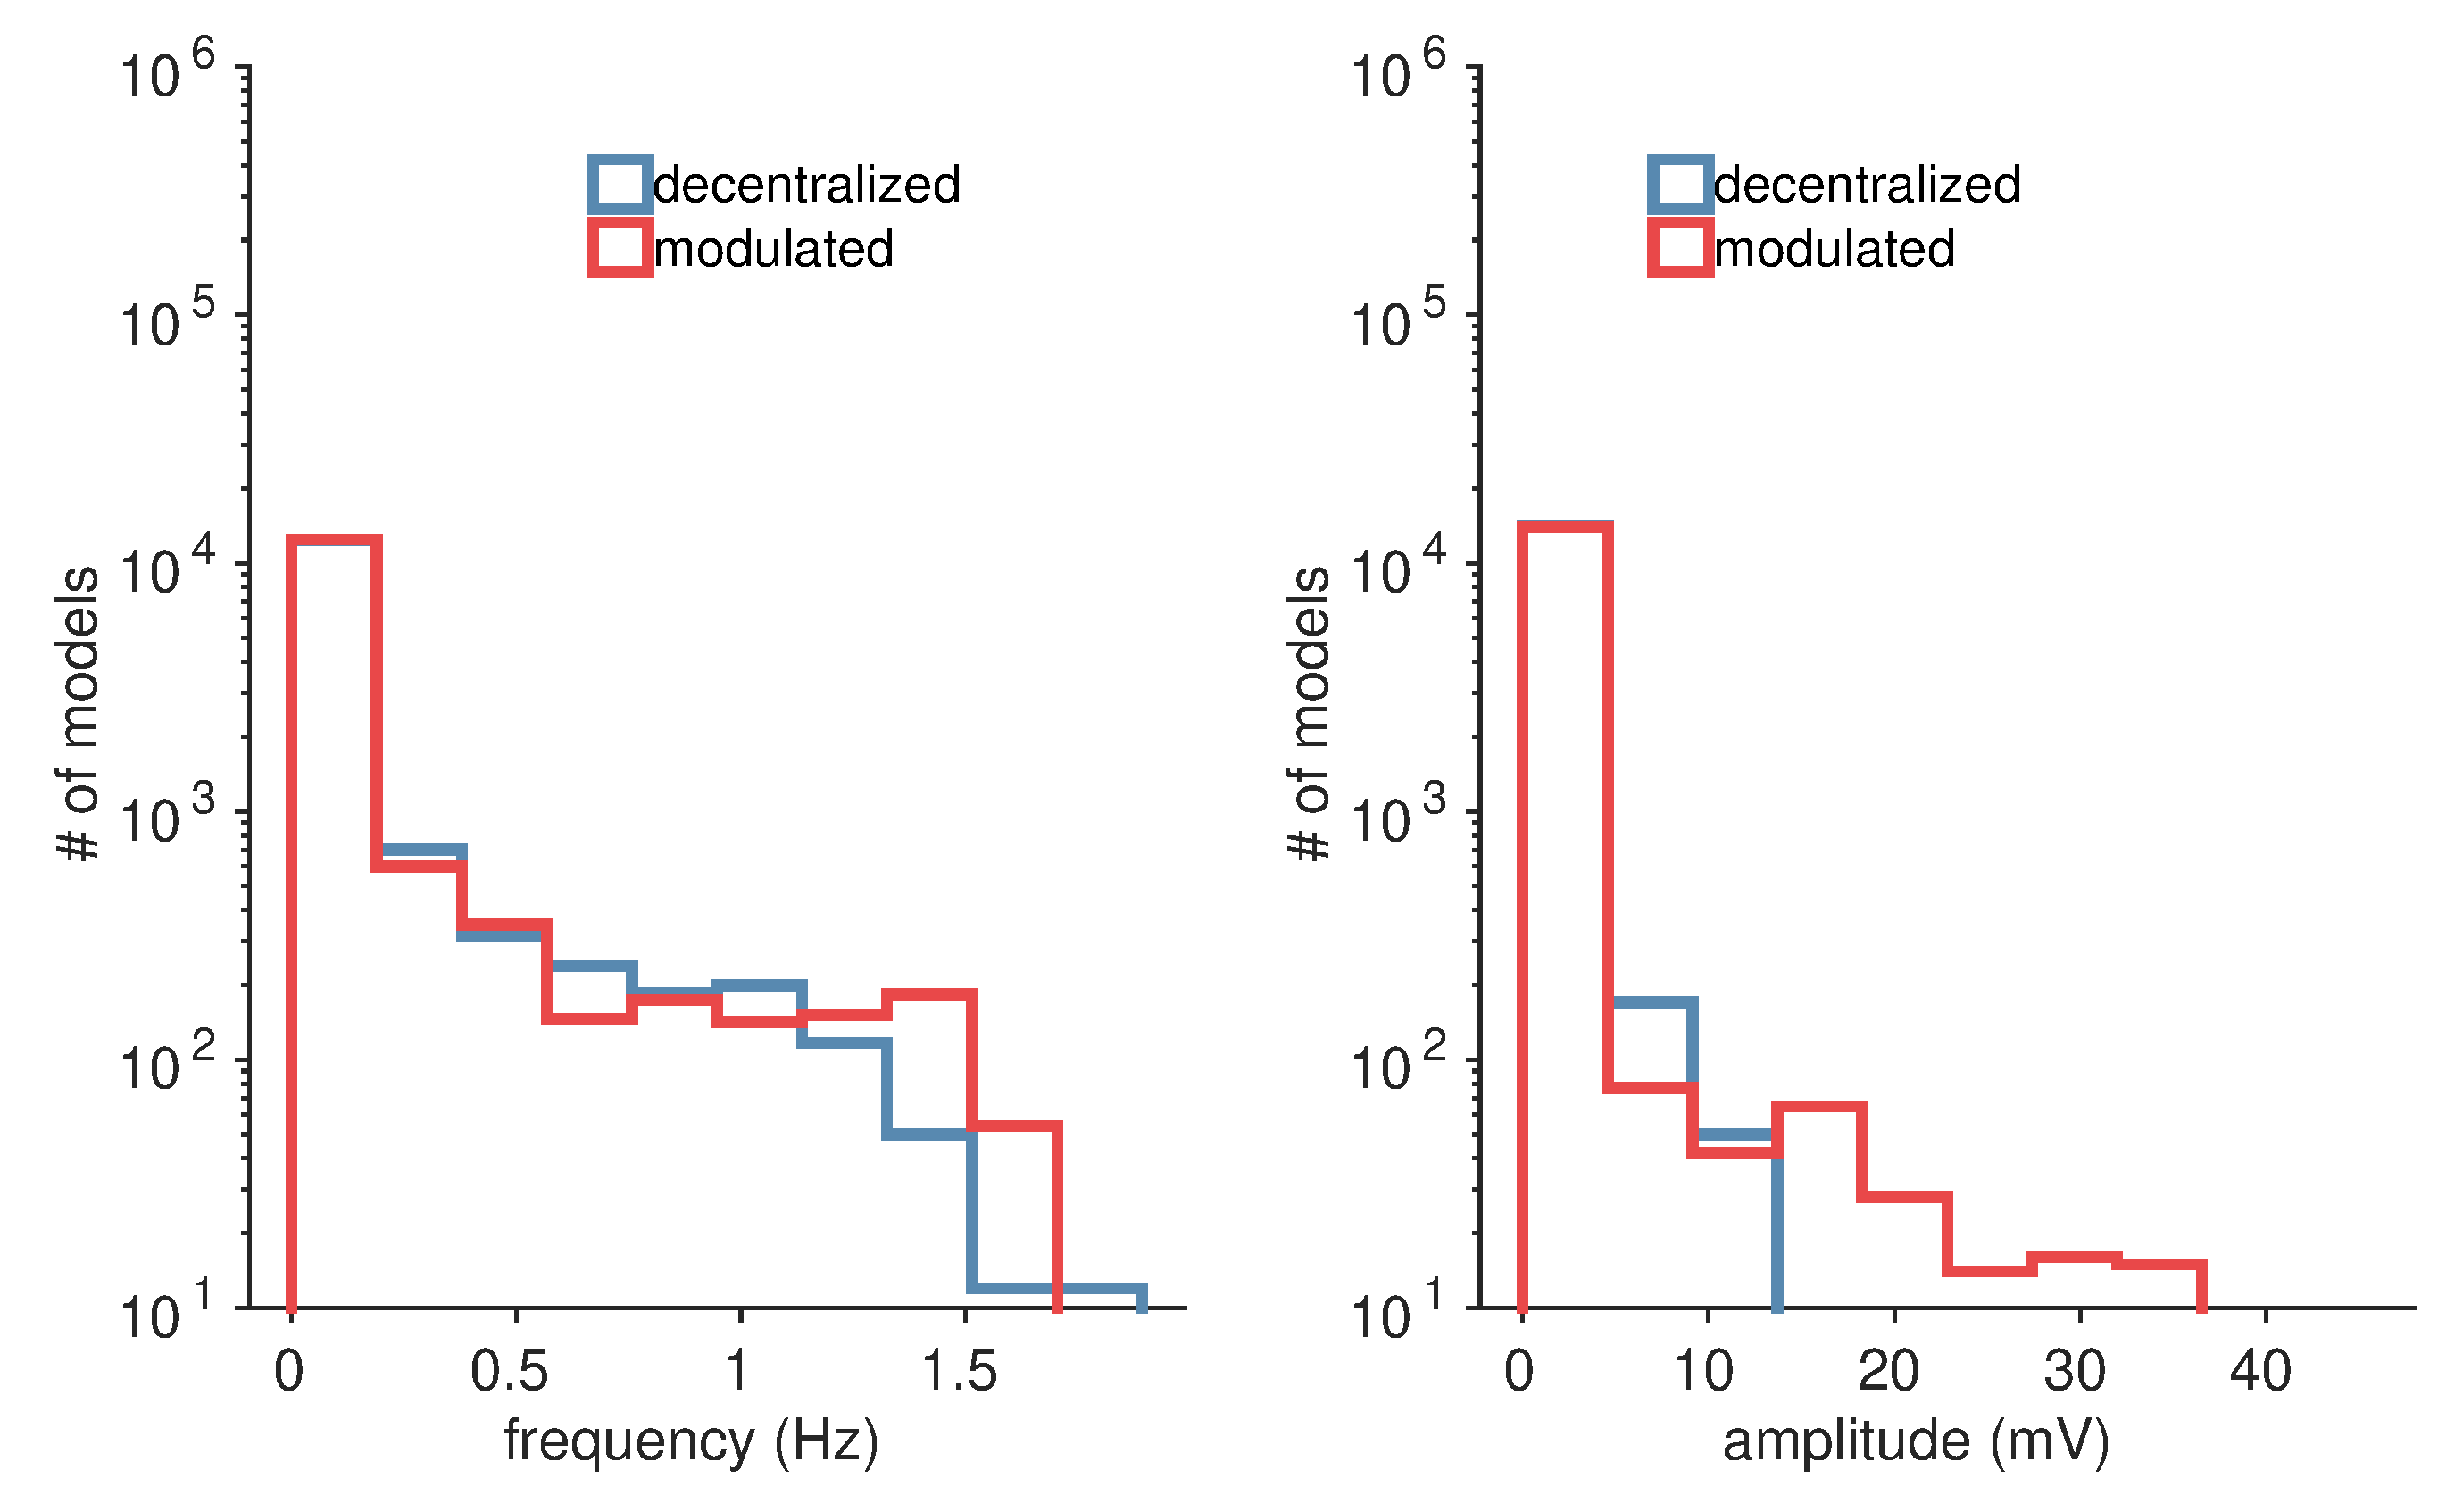
\includegraphics[width=1.0\linewidth]{gfx/prinz-models/histPrinz}
	\caption[Summary statistics of database models with modulatory input]{Most database models without \acs{INa} or \acs{ICaT} do not respond to modulatory input.}
	\label{fig:histprinz}
\end{figure}

Only a small subset of the models exhibited changes burst frequency and amplitude (\autoref{fig:histprinz}). \autoref{fig:traceprinz} illustrates three motifs in order of rarity. Most commonly, models with and without modulatory input were quiescent. A subset of models exhibited subthreshold voltage oscillations in both decentralized and modulated cases. The 1000 models with the greatest change in frequency and amplitude were replotted (\autoref{fig:prinzburstingmodelsnavcatexcisedswensen}). Models exhibit a sharp increase in peak voltage over a small range of modulatory input. Frequency increases monotonically sudden jumps in magnitude.

The 100 models which responded to modulatory input in a graded manner with increasing frequency and amplitude were optimized using a gradient descent algorithm (\autoref{fig:figprinzburstingttxcatnoscgmiswensenexprosim3}). Since the modulatory input IV curve achieves maximal inward current at $V_m \approx -32$ mV, peak voltage at high values of \acs{IMI} maximal conductance tended to be at least this membrane potential. A subset of models achieved graded frequency increase, though amplitude showed a sharply peaked jump from small oscillations (< 10 mV) to amplitude indicative of biological \acs{AB} neurons (\autoref{fig:figprinzburstingttxcatnoscgmiswensenexprosim3}). These data suggest that a subset of models experience modulatory input current as a bistable switch between non-oscillatory and oscillatory states.

When models were optimized over a smaller range of \acs{IMI} maximal conductance ($\bar{g}_{MI} = [0, 0.2]~\mu\mathrm{S/mm^2}$), resultant solutions responded to modulatory input in a graded manner. The burst frequency and amplitude increase smoothly as functions of modulatory input, responding most strongly at low maximal conductance. We hypothesize several reasons for this effect. First, the total capacitance of a physiologically-realistic \acs{AB} neuron is much higher than in the model neurons used here\autocite{Soto-TrevinoComputationalmodelelectrically2005,TurrigianoSelectiveregulationcurrent1995}. Second, the elimination of several currents significantly reduced the input resistance so that \acs{IMI} contributes a greater proportion to the net instantaneous current. Thirdly, most solutions converged to small values of conductances. Since the membrane potential evolves proportionally to the instantaneous sum of the currents, relative proportions of conductance with respect to each other and the membrane capacitance determine the dynamics. A model neuron with small membrane capacitance and intrinsic conductances produces qualitatively different activity with smaller perturbations.

\begin{figure}
	\centering
	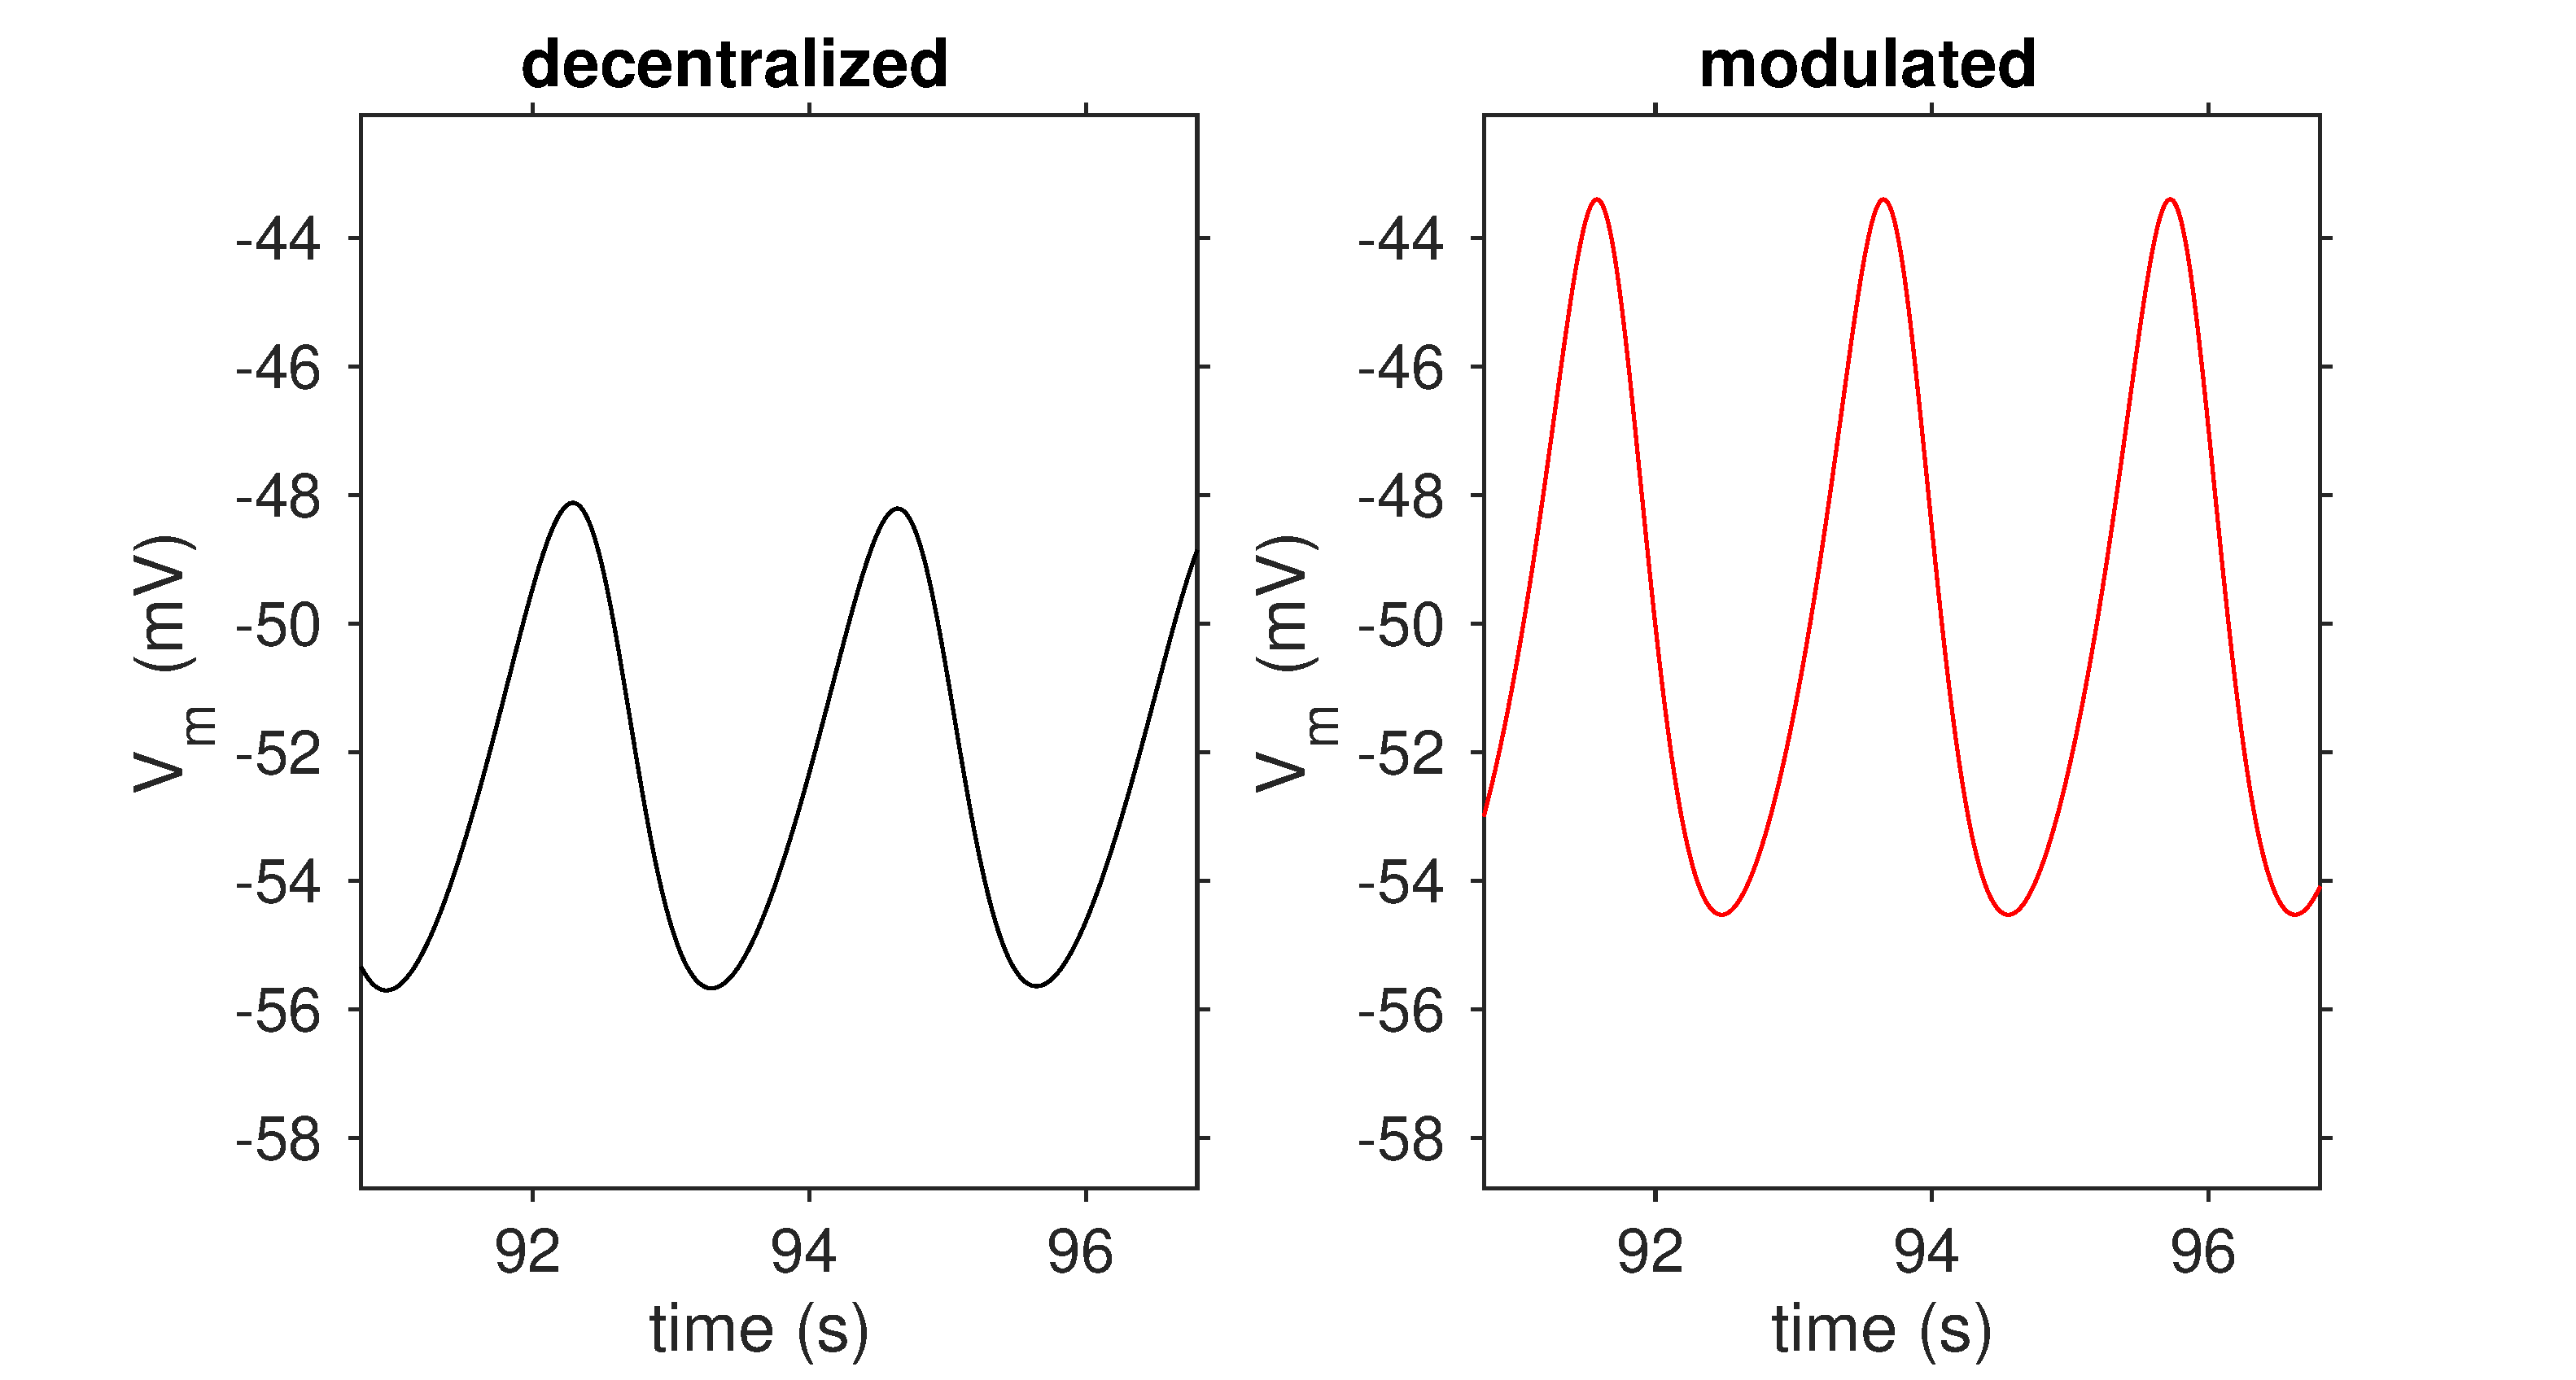
\includegraphics[width=1.0\linewidth]{gfx/prinz-models/ABwmod2}
	\caption[Superimposed model AB traces]{\acs{AB} model increases in amplitude and frequency with modulatory input. The model recapitulates electrophysiological recordings (\autoref{fig:sharp2}). Modulatory input current cannot replace slow calcium in its excitatory role, but a balance between \acs{IH}, \acs{ICaS}, and outward currents produce the conditions for \acs{IMI} to depolarize the membrane potential during voltage peaks.}
	\label{fig:abwmod}
\end{figure}

\FloatBarrier

\section{Variability in Network Response to Modulation}
\acs{RPCH} activates \ac{IMI} in the anterior burster (\acs{AB}) and lateral pyloric (\acs{LP}) cells of the \acs{STG}\autocite{NusbaumNeuronalRoleCrustacean1988}. To model the effects of \acs{RPCH} modulation in the pyloric circuit, \acs{IMI} was added to each cell and together in the network model (\autoref{fig:pyloriccircuit}) with \acs{AB} and \acsp{PD} reduced to a single composite pacemaker neuron (\acs{AB}-\acs{PD}). Particle swarm optimization (\autoref{sec:parameteroptimization}) selected for models which increased in burst frequency and slow wave amplitude over increasing modulatory input into \acs{AB}-\acs{PD}, \acs{LP}, and both model neurons. Maximal conductances for all ionic and synaptic currents were varied as parameters (28 parameters plus one for each cell with \acs{IMI}).

\subsection{Neuromodulation Increases Frequency and Amplitude}
Optimization produced models of the network with increased burst frequency and slow wave amplitude under modulation in the three conditions. Three motifs of network activity appeared several times in optimized solutions. Some model networks produced triphasic activity without modulation, and increased burst frequency and slow wave amplitude under neuromodulation. Others produced periodic, but not pyloric activity (e.g. skipped bursts) and rectified these errors under modulation. The third category contained quiescent and tonically-firing networks which become pyloric under modulation.

\autoref{fig:networkab47traces} displays an optimized network model with modulatory input into \acs{AB}-\acs{PD}. Without modulation, the network is stable, with a triphasic rhythm. Addition of modulatory input monotonically increases the burst frequency. The duty cycle for \acs{PY} decreases from 0.5 to 0.3. Similarly, the mean number of spikes per burst in \acs{PY} decreases. This indicates that the burst duration is decreasing and the mean inter-spike interval remains relatively constant. \acs{PY} is not able to increase in slow-wave amplitude until the duration and intensity of the bursts can be maintained at the higher frequency. 

\begin{figure}[h]
	\centering
	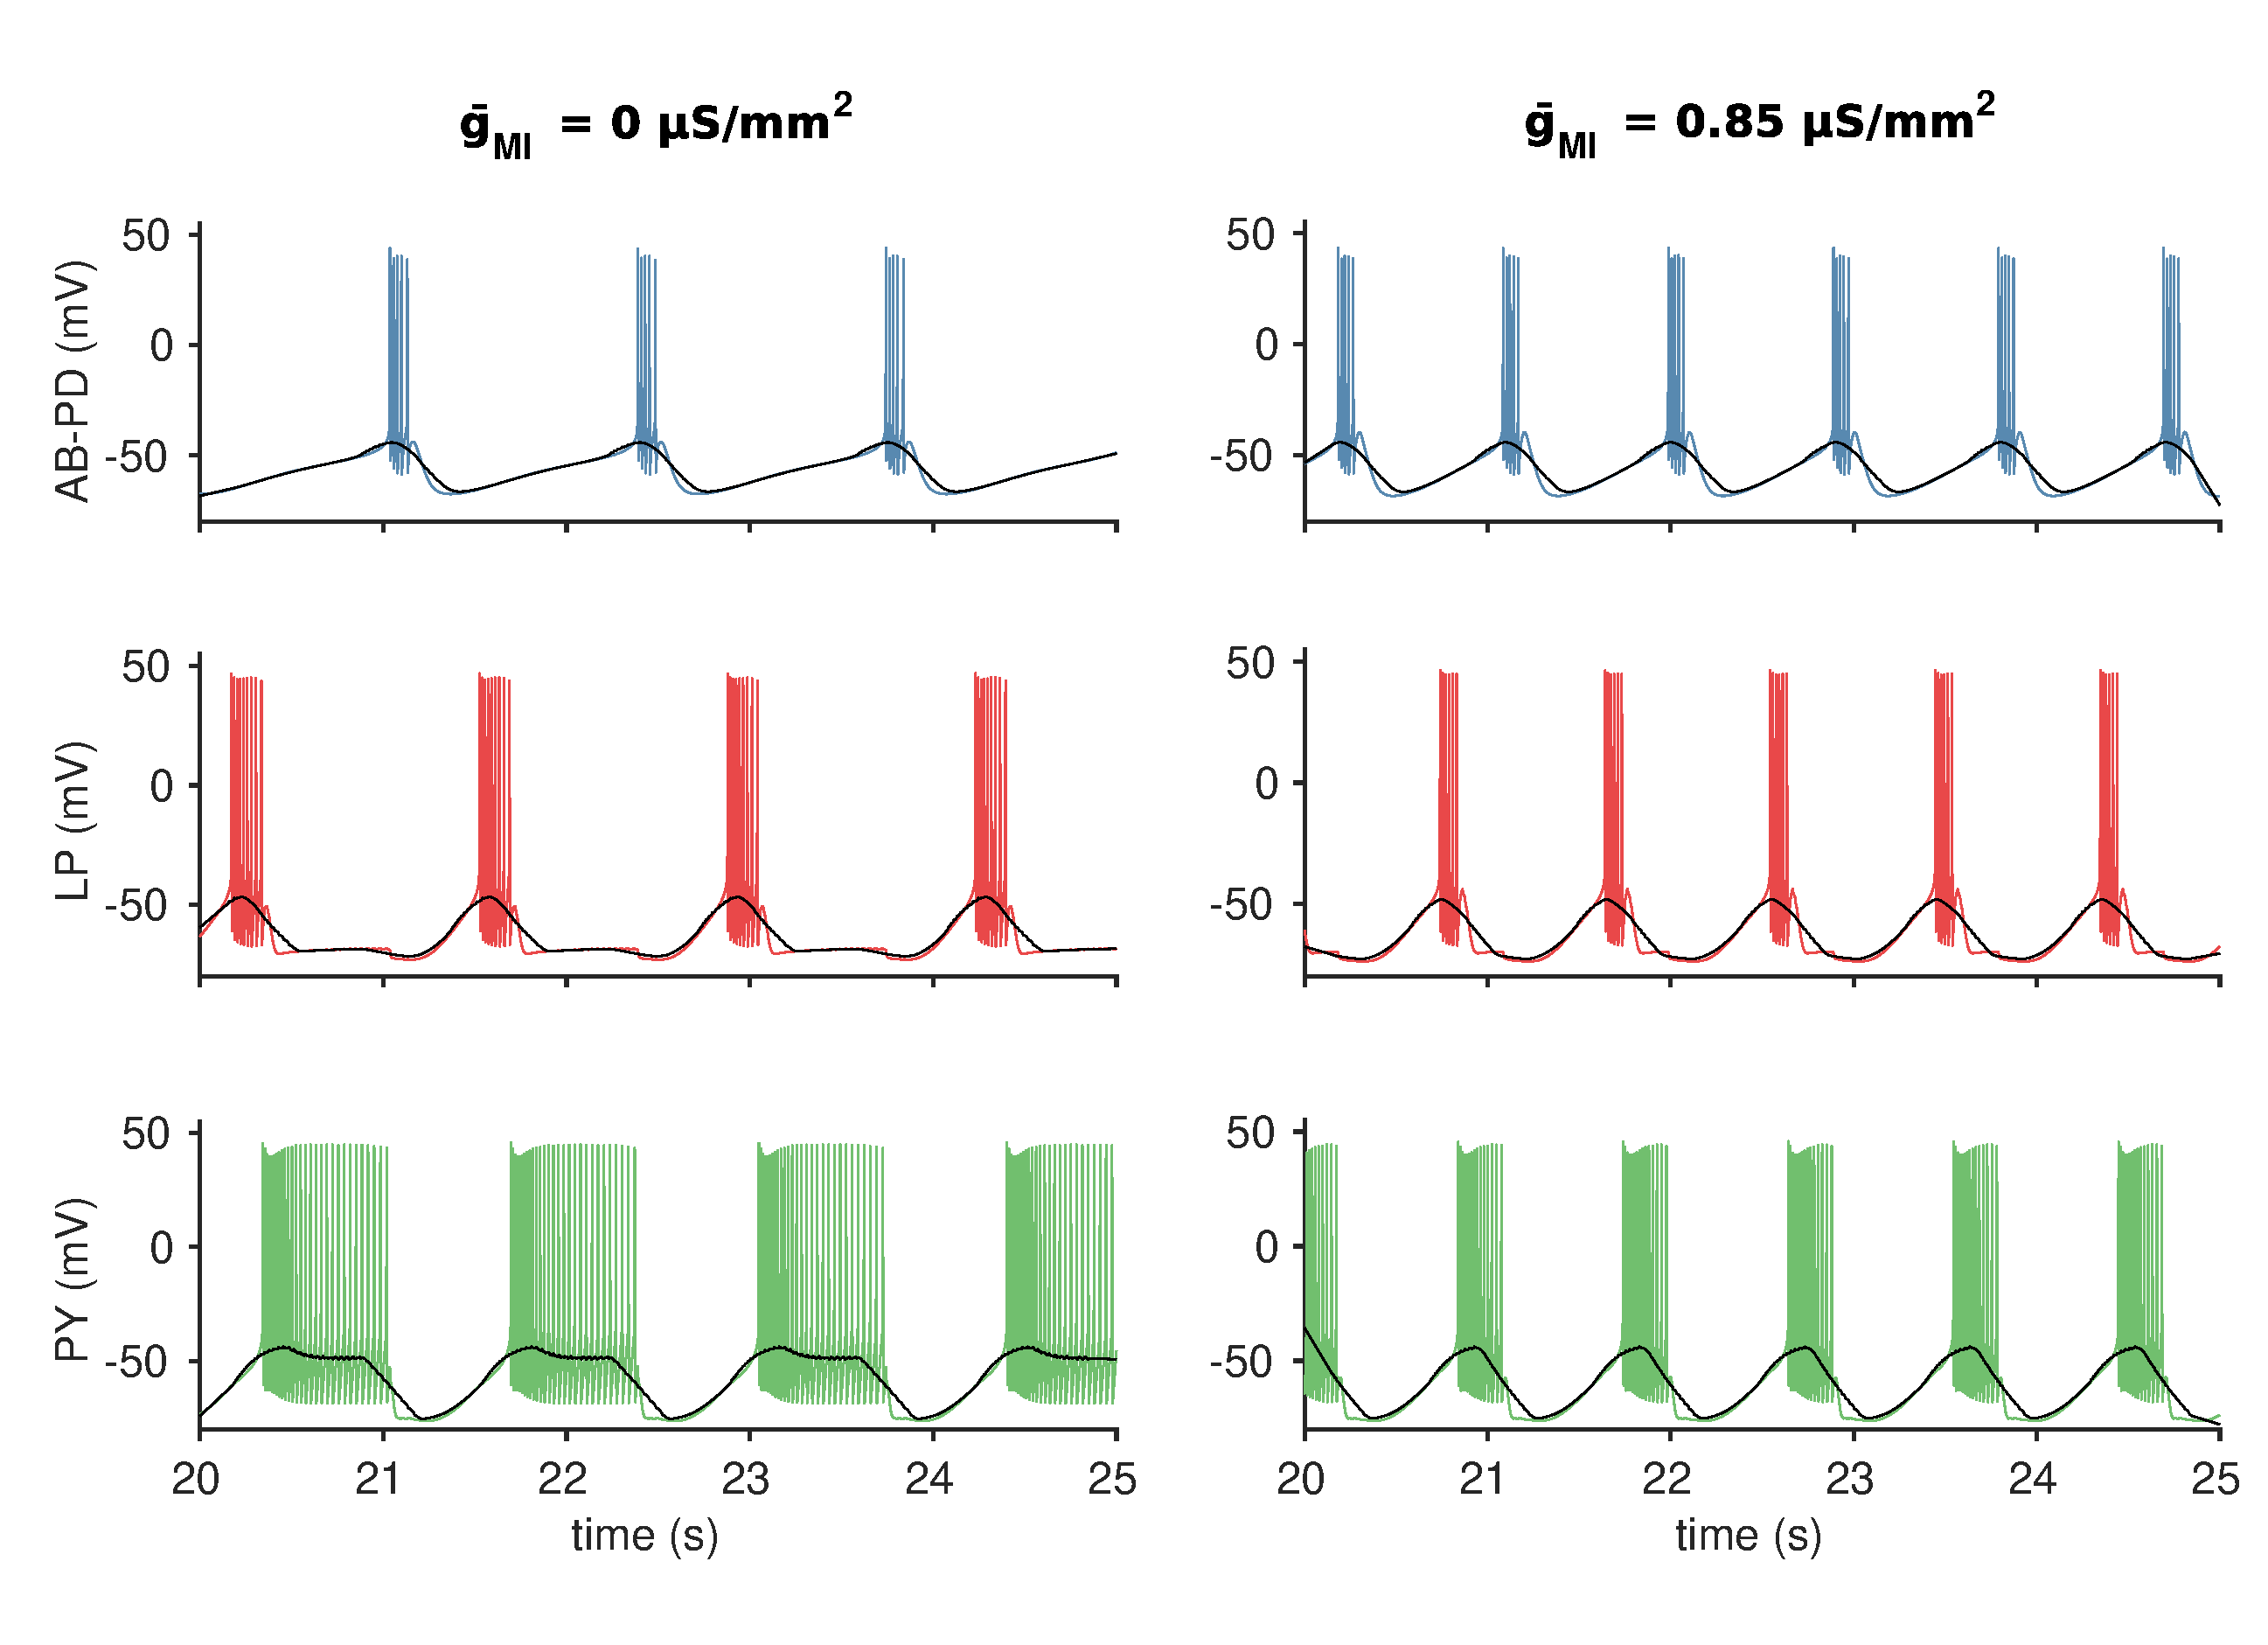
\includegraphics[width=1.0\linewidth]{gfx/network/network_AB_47_traces}
	\caption[Network with modulation into AB-PD (traces)]{Modulation into \acs{AB}-\acs{PD} increases burst frequency and \acs{AB}-\acs{PD} slow wave amplitude. Left-hand traces are without neuromodulation.. Right-hand traces have \acs{IMI} in \acs{AB}-\acs{PD} at $\bar{g}_{MI} = 0.85~\mu \mathrm{S/mm^2}$. Colors indicate cells (blue is \acs{AB}-\acs{PD}, red is \acs{LP}, green is \acs{PY} and overlaid black indicates the slow wave).}
	\label{fig:networkab47traces}
\end{figure}

\begin{figure}[h]
	\centering
	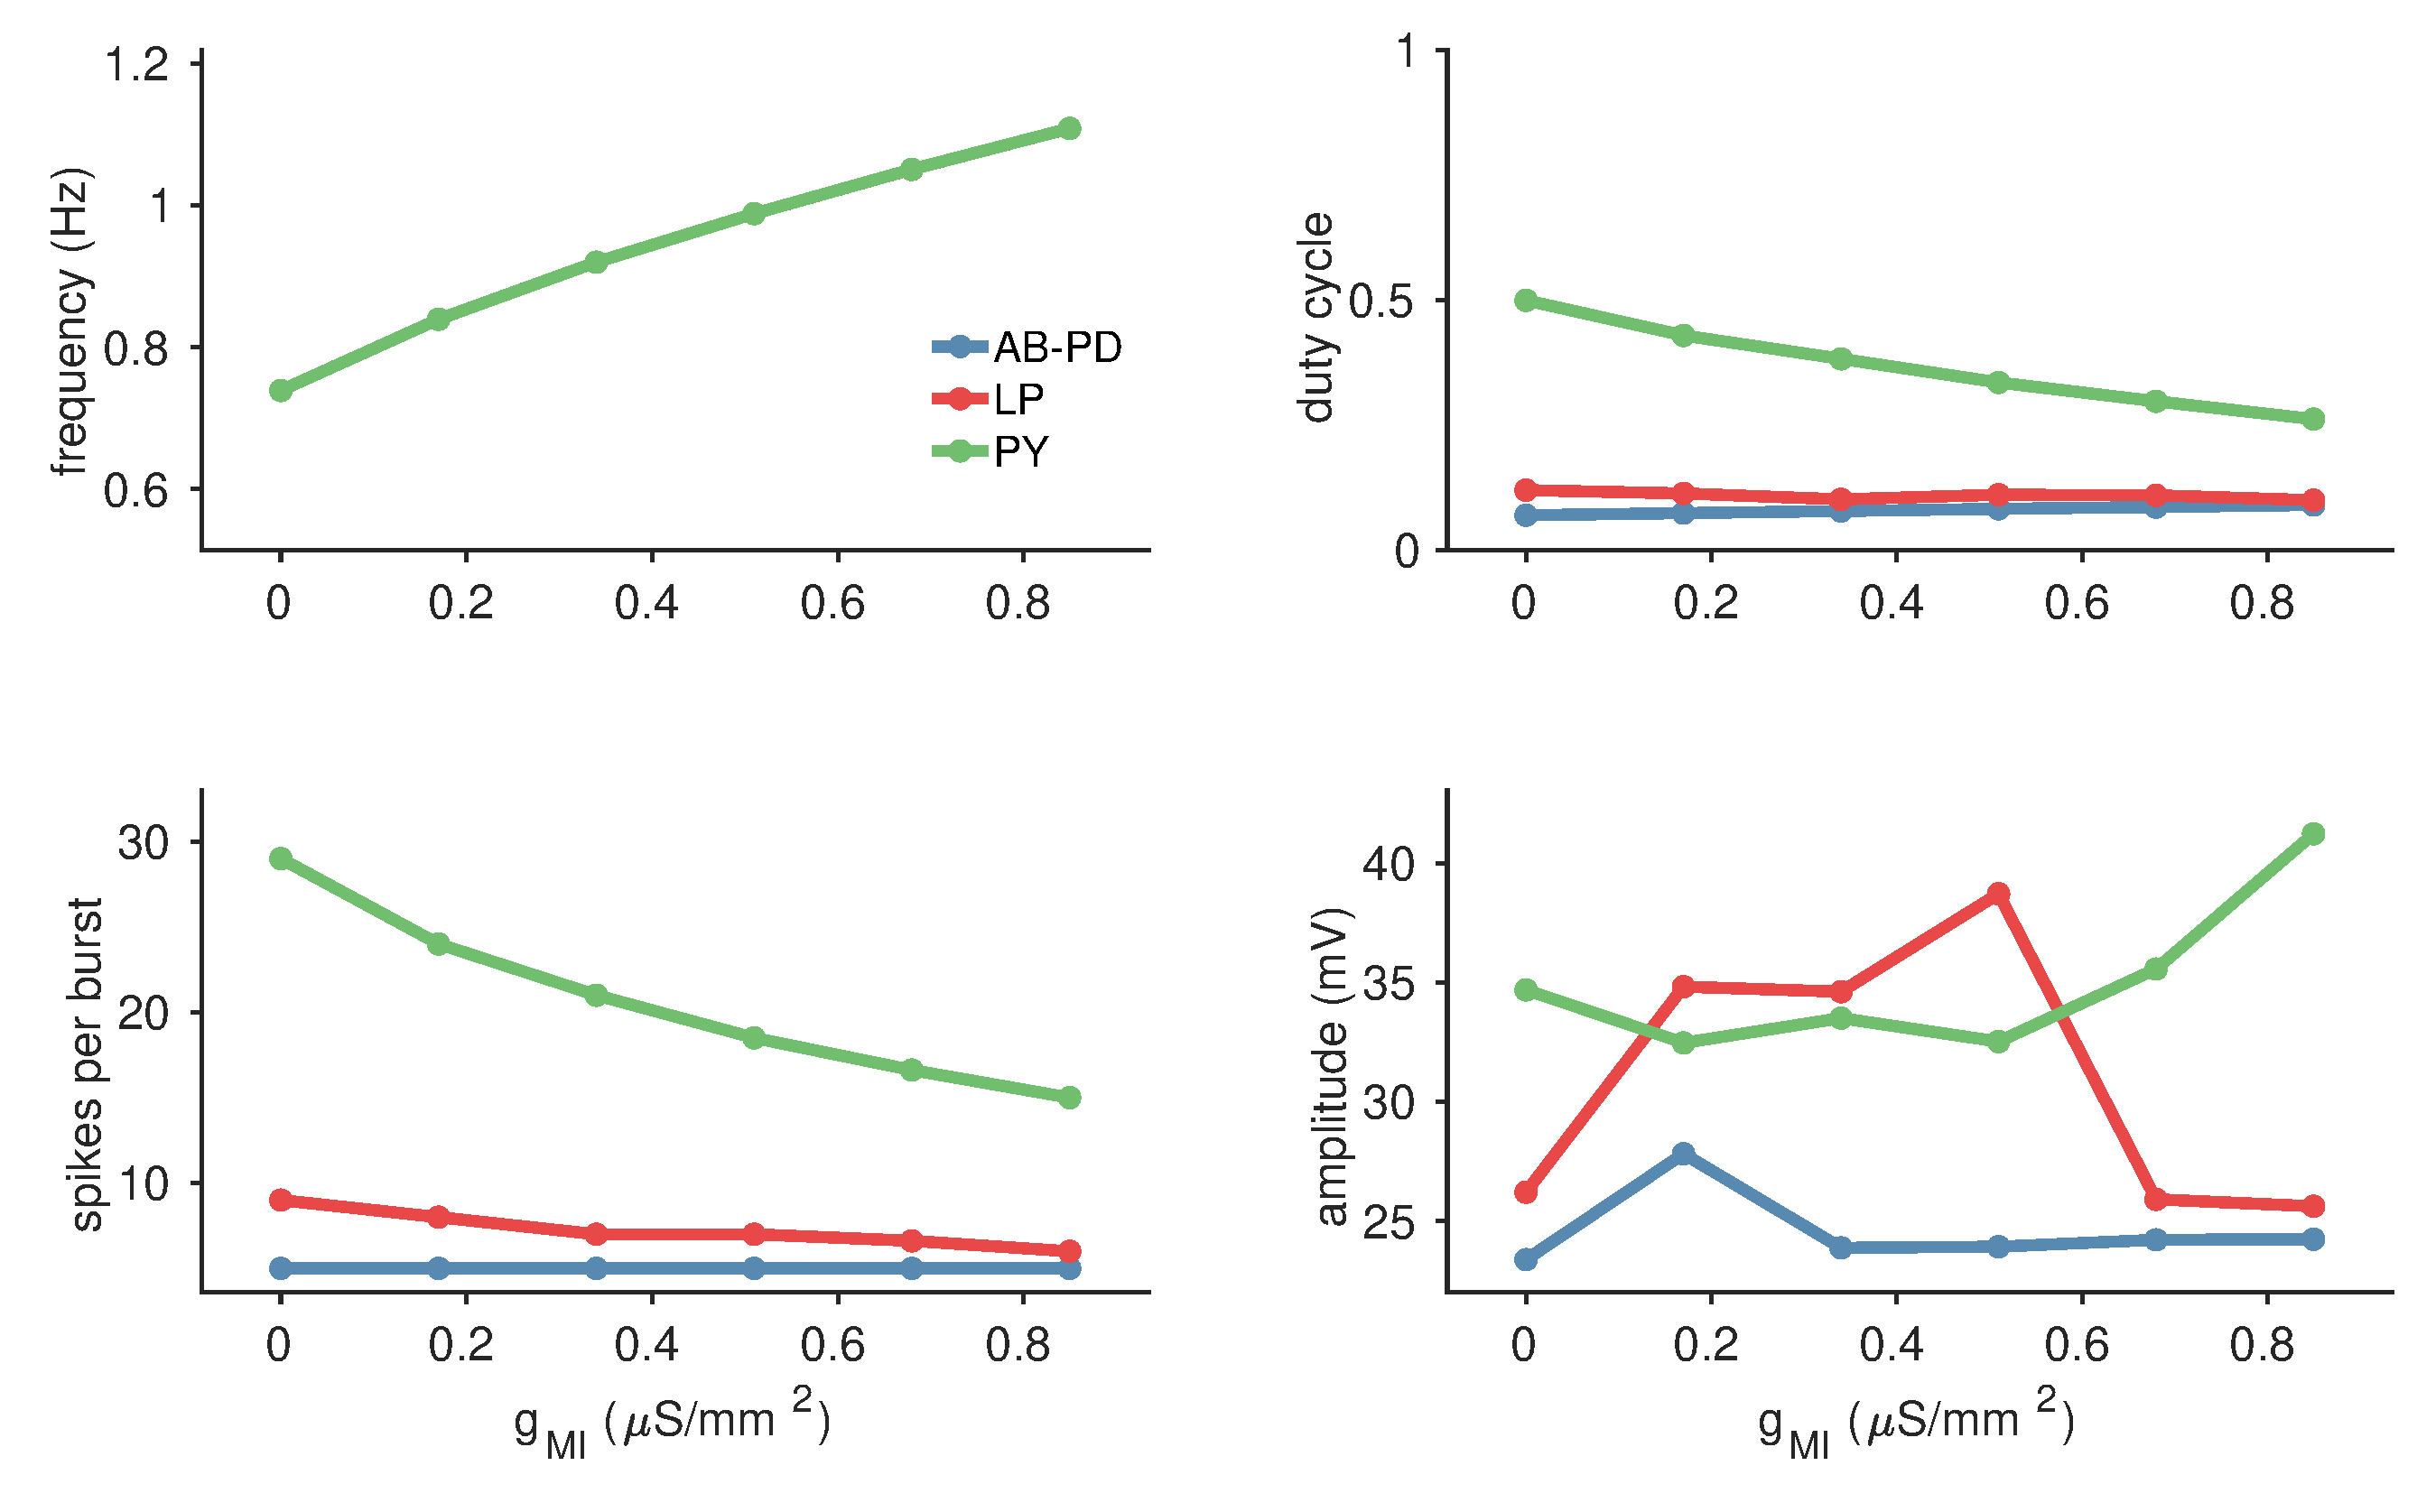
\includegraphics[width=1.0\linewidth]{gfx/network/network_AB_47_metrics}
	\caption[Network with modulation into AB-PD (metrics)]{Modulation into \acs{AB}-\acs{PD} increases burst frequency and \acs{AB}-\acs{PD} slow wave amplitude. Metrics at steady-state as a function of increasing modulatory input. Colors indicate cells (blue is \acs{AB}-\acs{PD}, red is \acs{LP}, green is \acs{PY}.}
	\label{fig:networkab47metrics}
\end{figure}

\FloatBarrier

\begin{figure}[h]
	\centering
	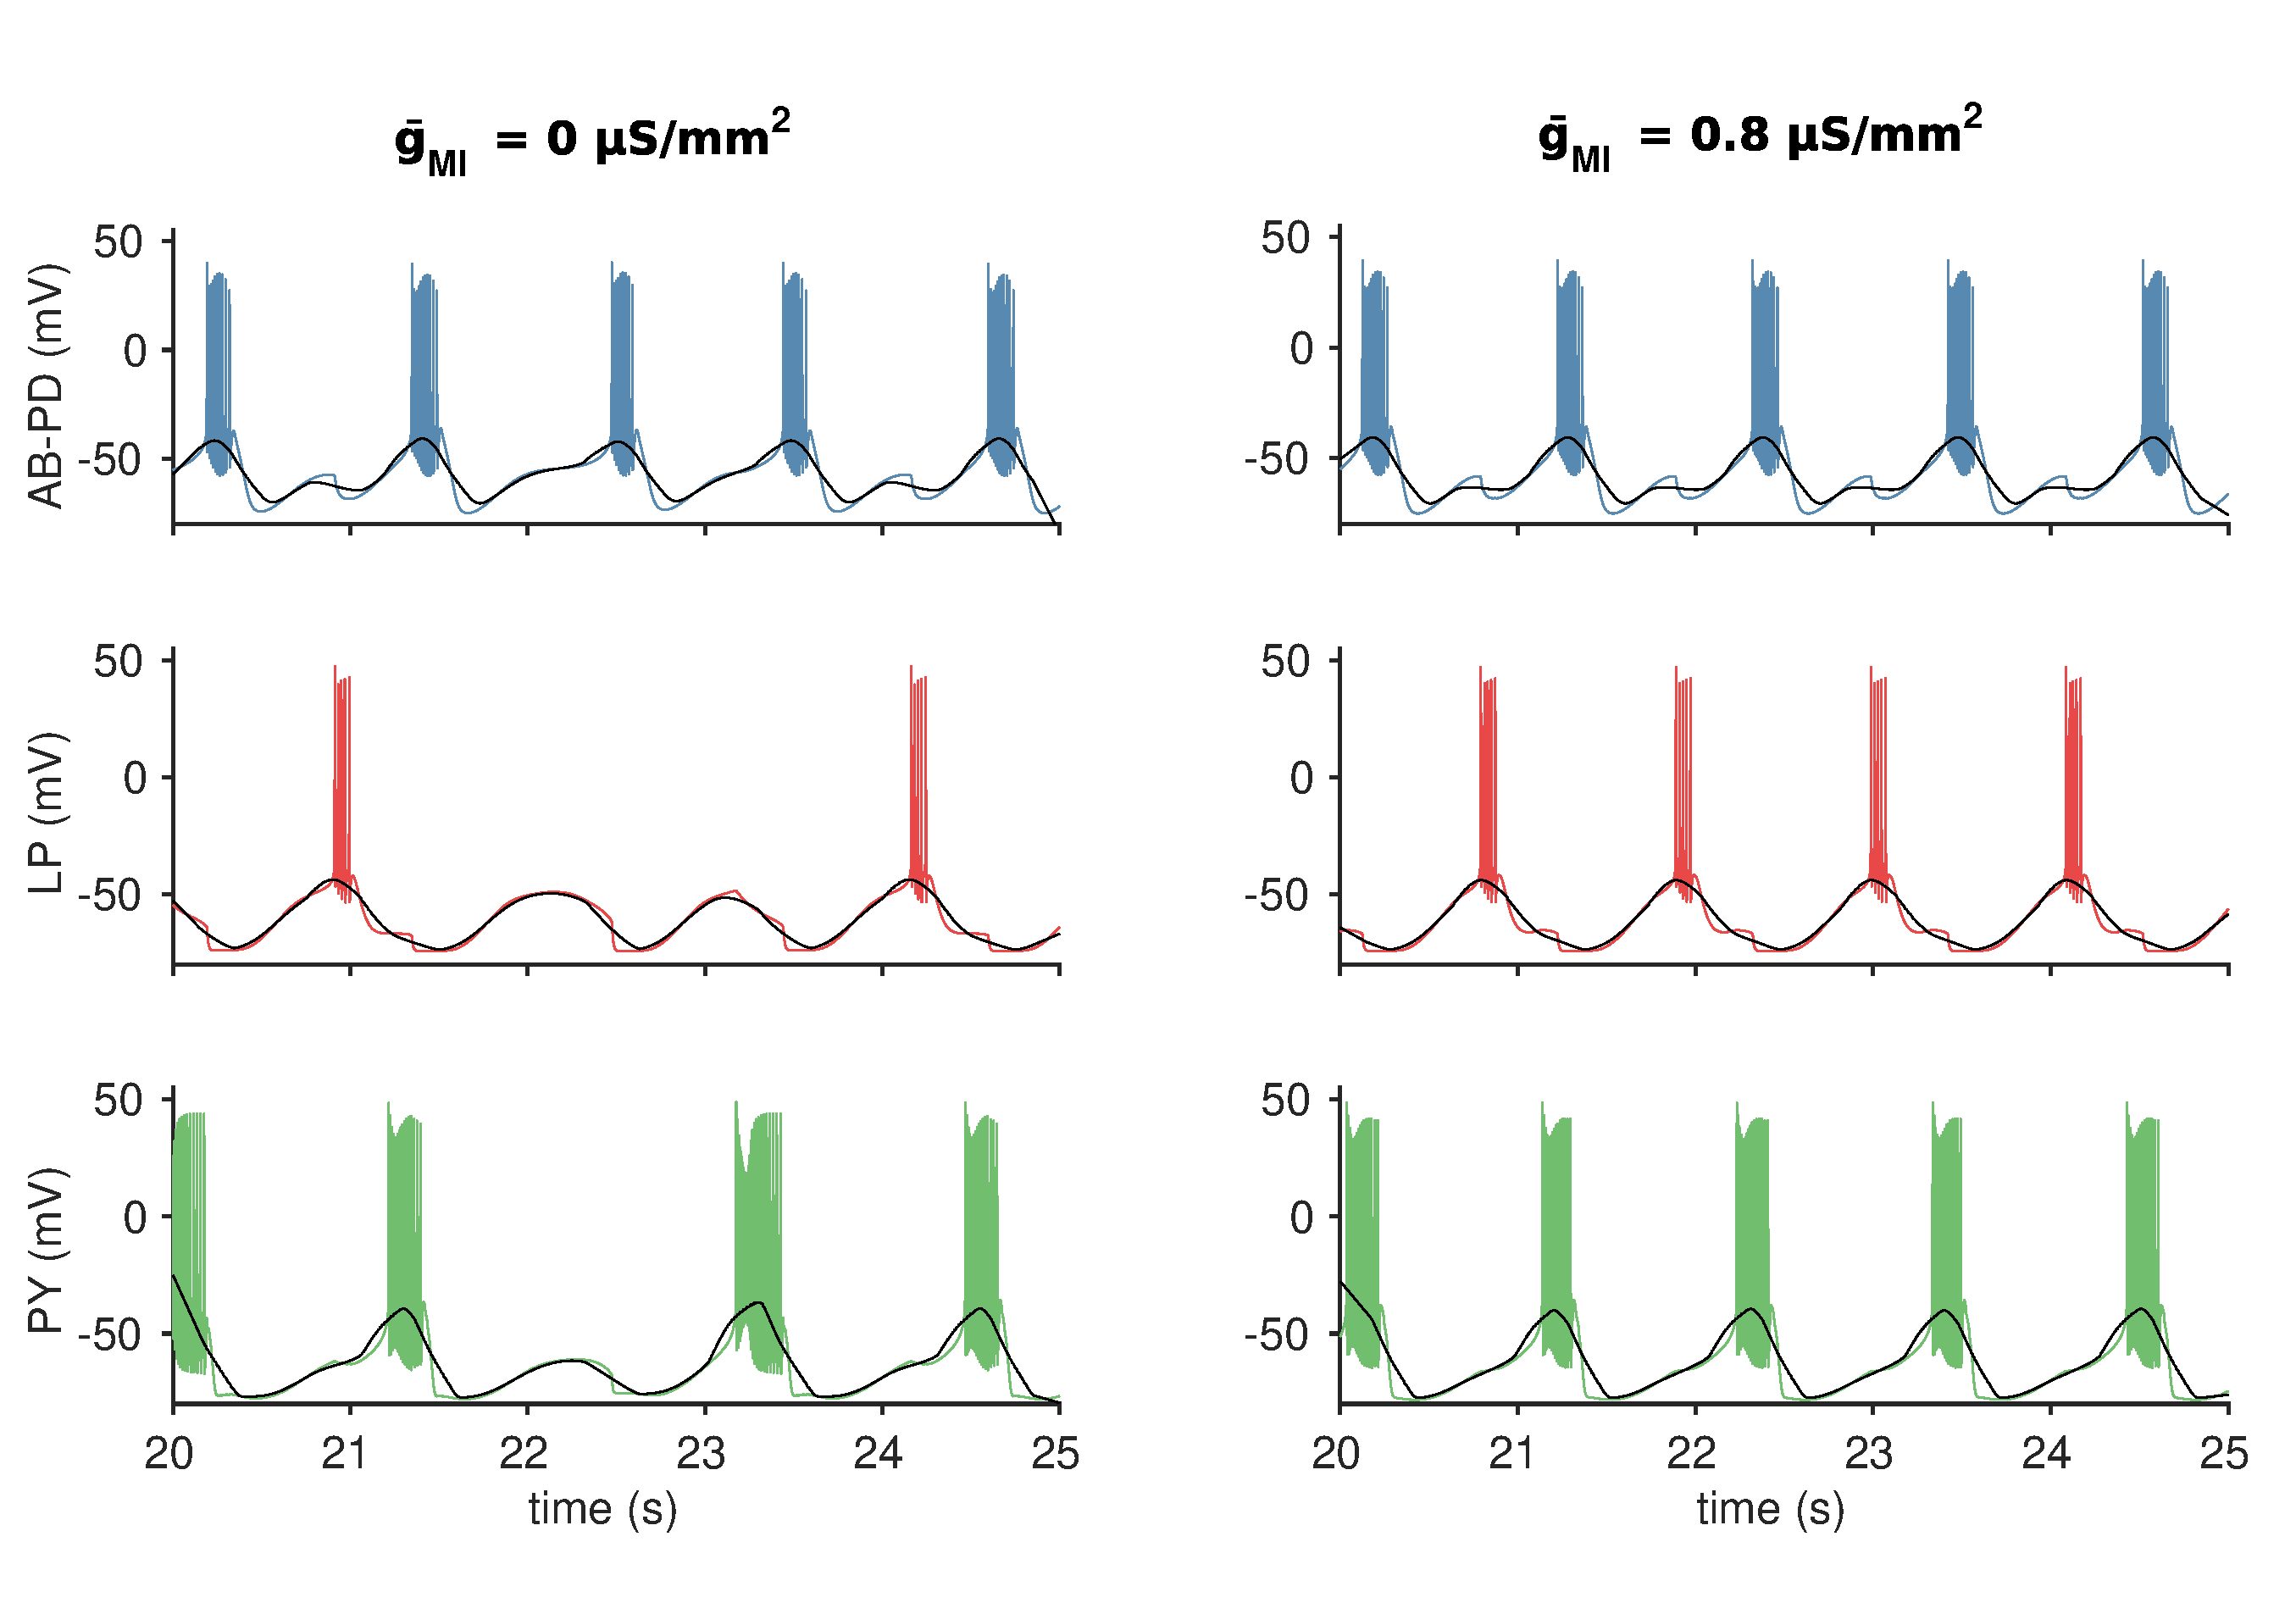
\includegraphics[width=1.0\linewidth]{gfx/network/network_LP_28_traces}
	\caption[Network with modulation into LP (traces)]{Modulation into \acs{LP} rescues abnormal activity. Modulation into \acs{LP} increases burst frequency and \acs{AB}-\acs{PD} slow wave amplitude. Left-hand traces are without neuromodulation. Right-hand traces have \acs{IMI} in \acs{LP} at $\bar{g}_{MI} = 0.8~\mu \mathrm{S/mm^2}$. Colors indicate cells (blue is \acs{AB}-\acs{PD}, red is \acs{LP}, green is \acs{PY} and overlaid black indicates the slow wave).}
	\label{fig:networklp28traces}
\end{figure}

\begin{figure}[h]
	\centering
	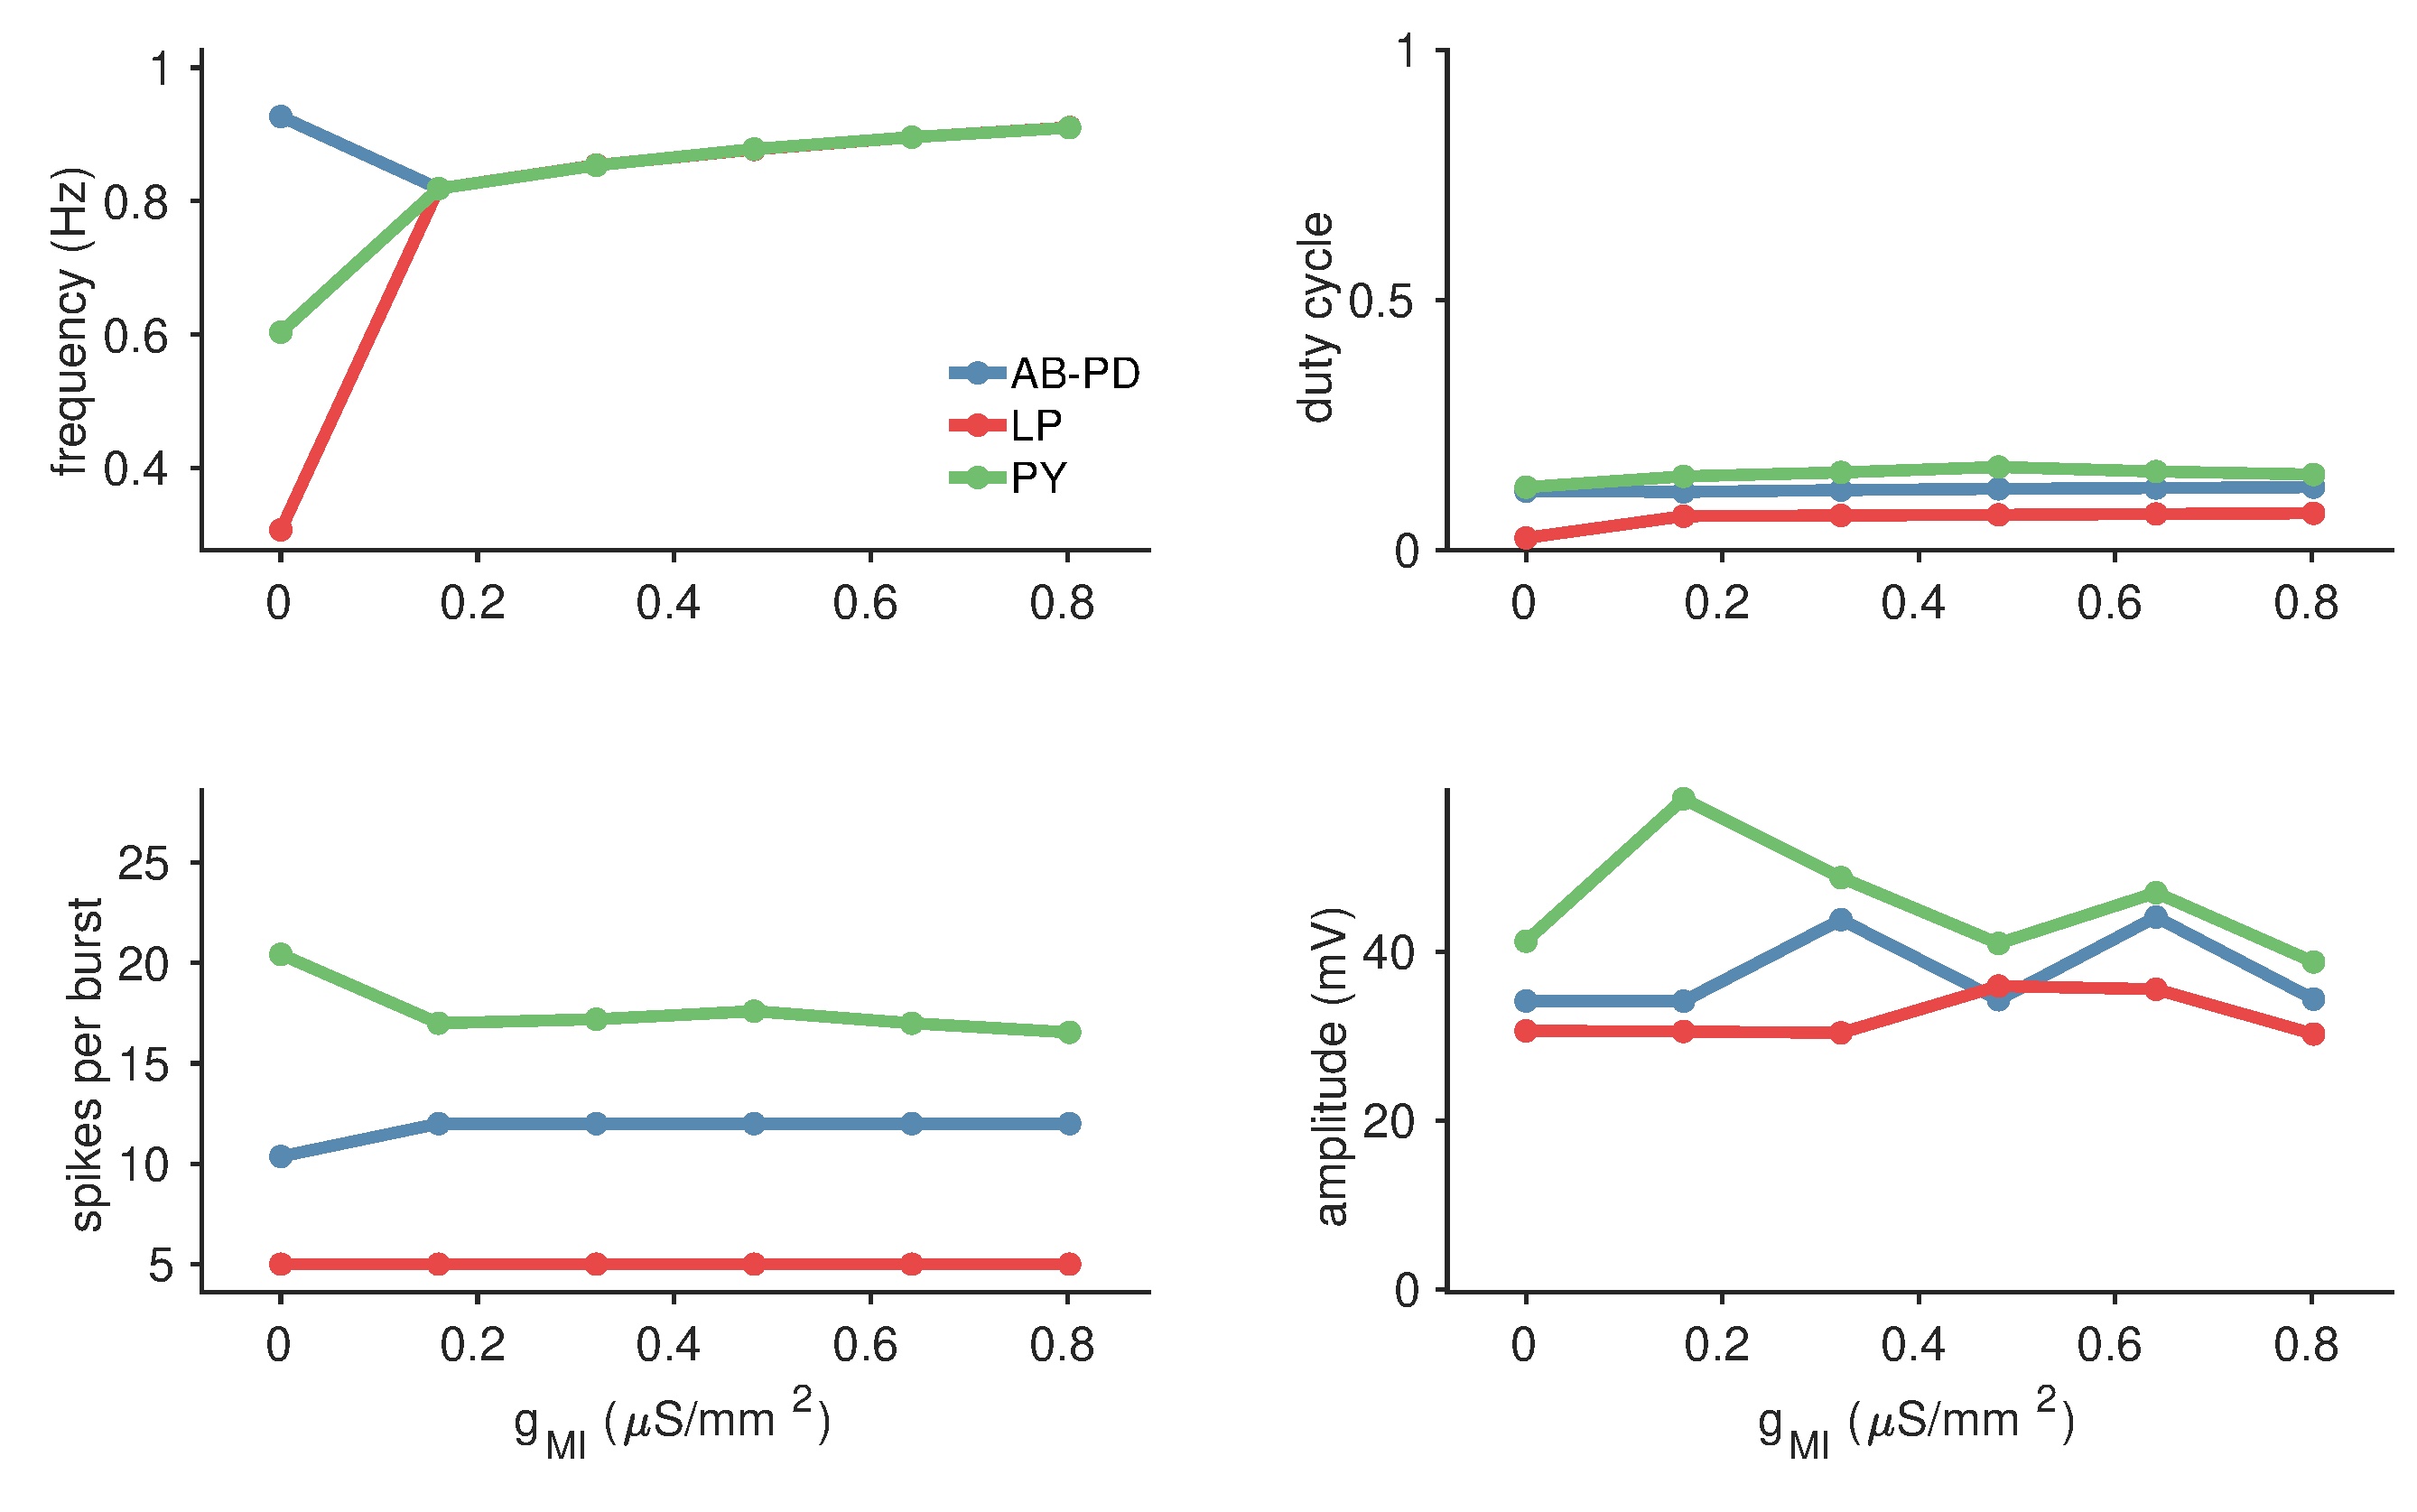
\includegraphics[width=1.0\linewidth]{gfx/network/network_LP_28_metrics}
	\caption[Network with modulation into LP (metrics)]{Modulation into \acs{LP} rescues abnormal activity. Modulation into \acs{AB}-\acs{PD} increases burst frequency and \acs{AB}-\acs{PD} slow wave amplitude. Metrics at steady-state as a function of increasing modulatory input. Colors indicate cells (blue is \acs{AB}-\acs{PD}, red is \acs{LP}, green is \acs{PY}).}
	\label{fig:networklp28metrics}
\end{figure}

\FloatBarrier

Models can recapitulate loss of triphasic rhythm with decentralization. In \autoref{fig:networklp28traces}, modulation into \acs{LP} corrects a network with burst asymmetry. After the network is brought back into rhythm, increasing modulation increases the burst frequency. Since all bursts are short in duration, the duty cycle does not change. The slow wave amplitude in \acs{AB}-\acs{PD} depends on the phase relationship between \acs{AB}-\acs{PD} and \acs{LP}, which itself depends on the maximal conductance of \acs{IMI} in \acs{LP}. When the burst in \acs{LP} occurs immediately following the termination of the burst in \acs{AB}-\acs{PD}, allowing more time between the termination of the burst in \acs{LP} and the next in \acs{AB}-\acs{PD} the amplitude in the pacemaker is greater.

\begin{figure}[h]
	\centering
	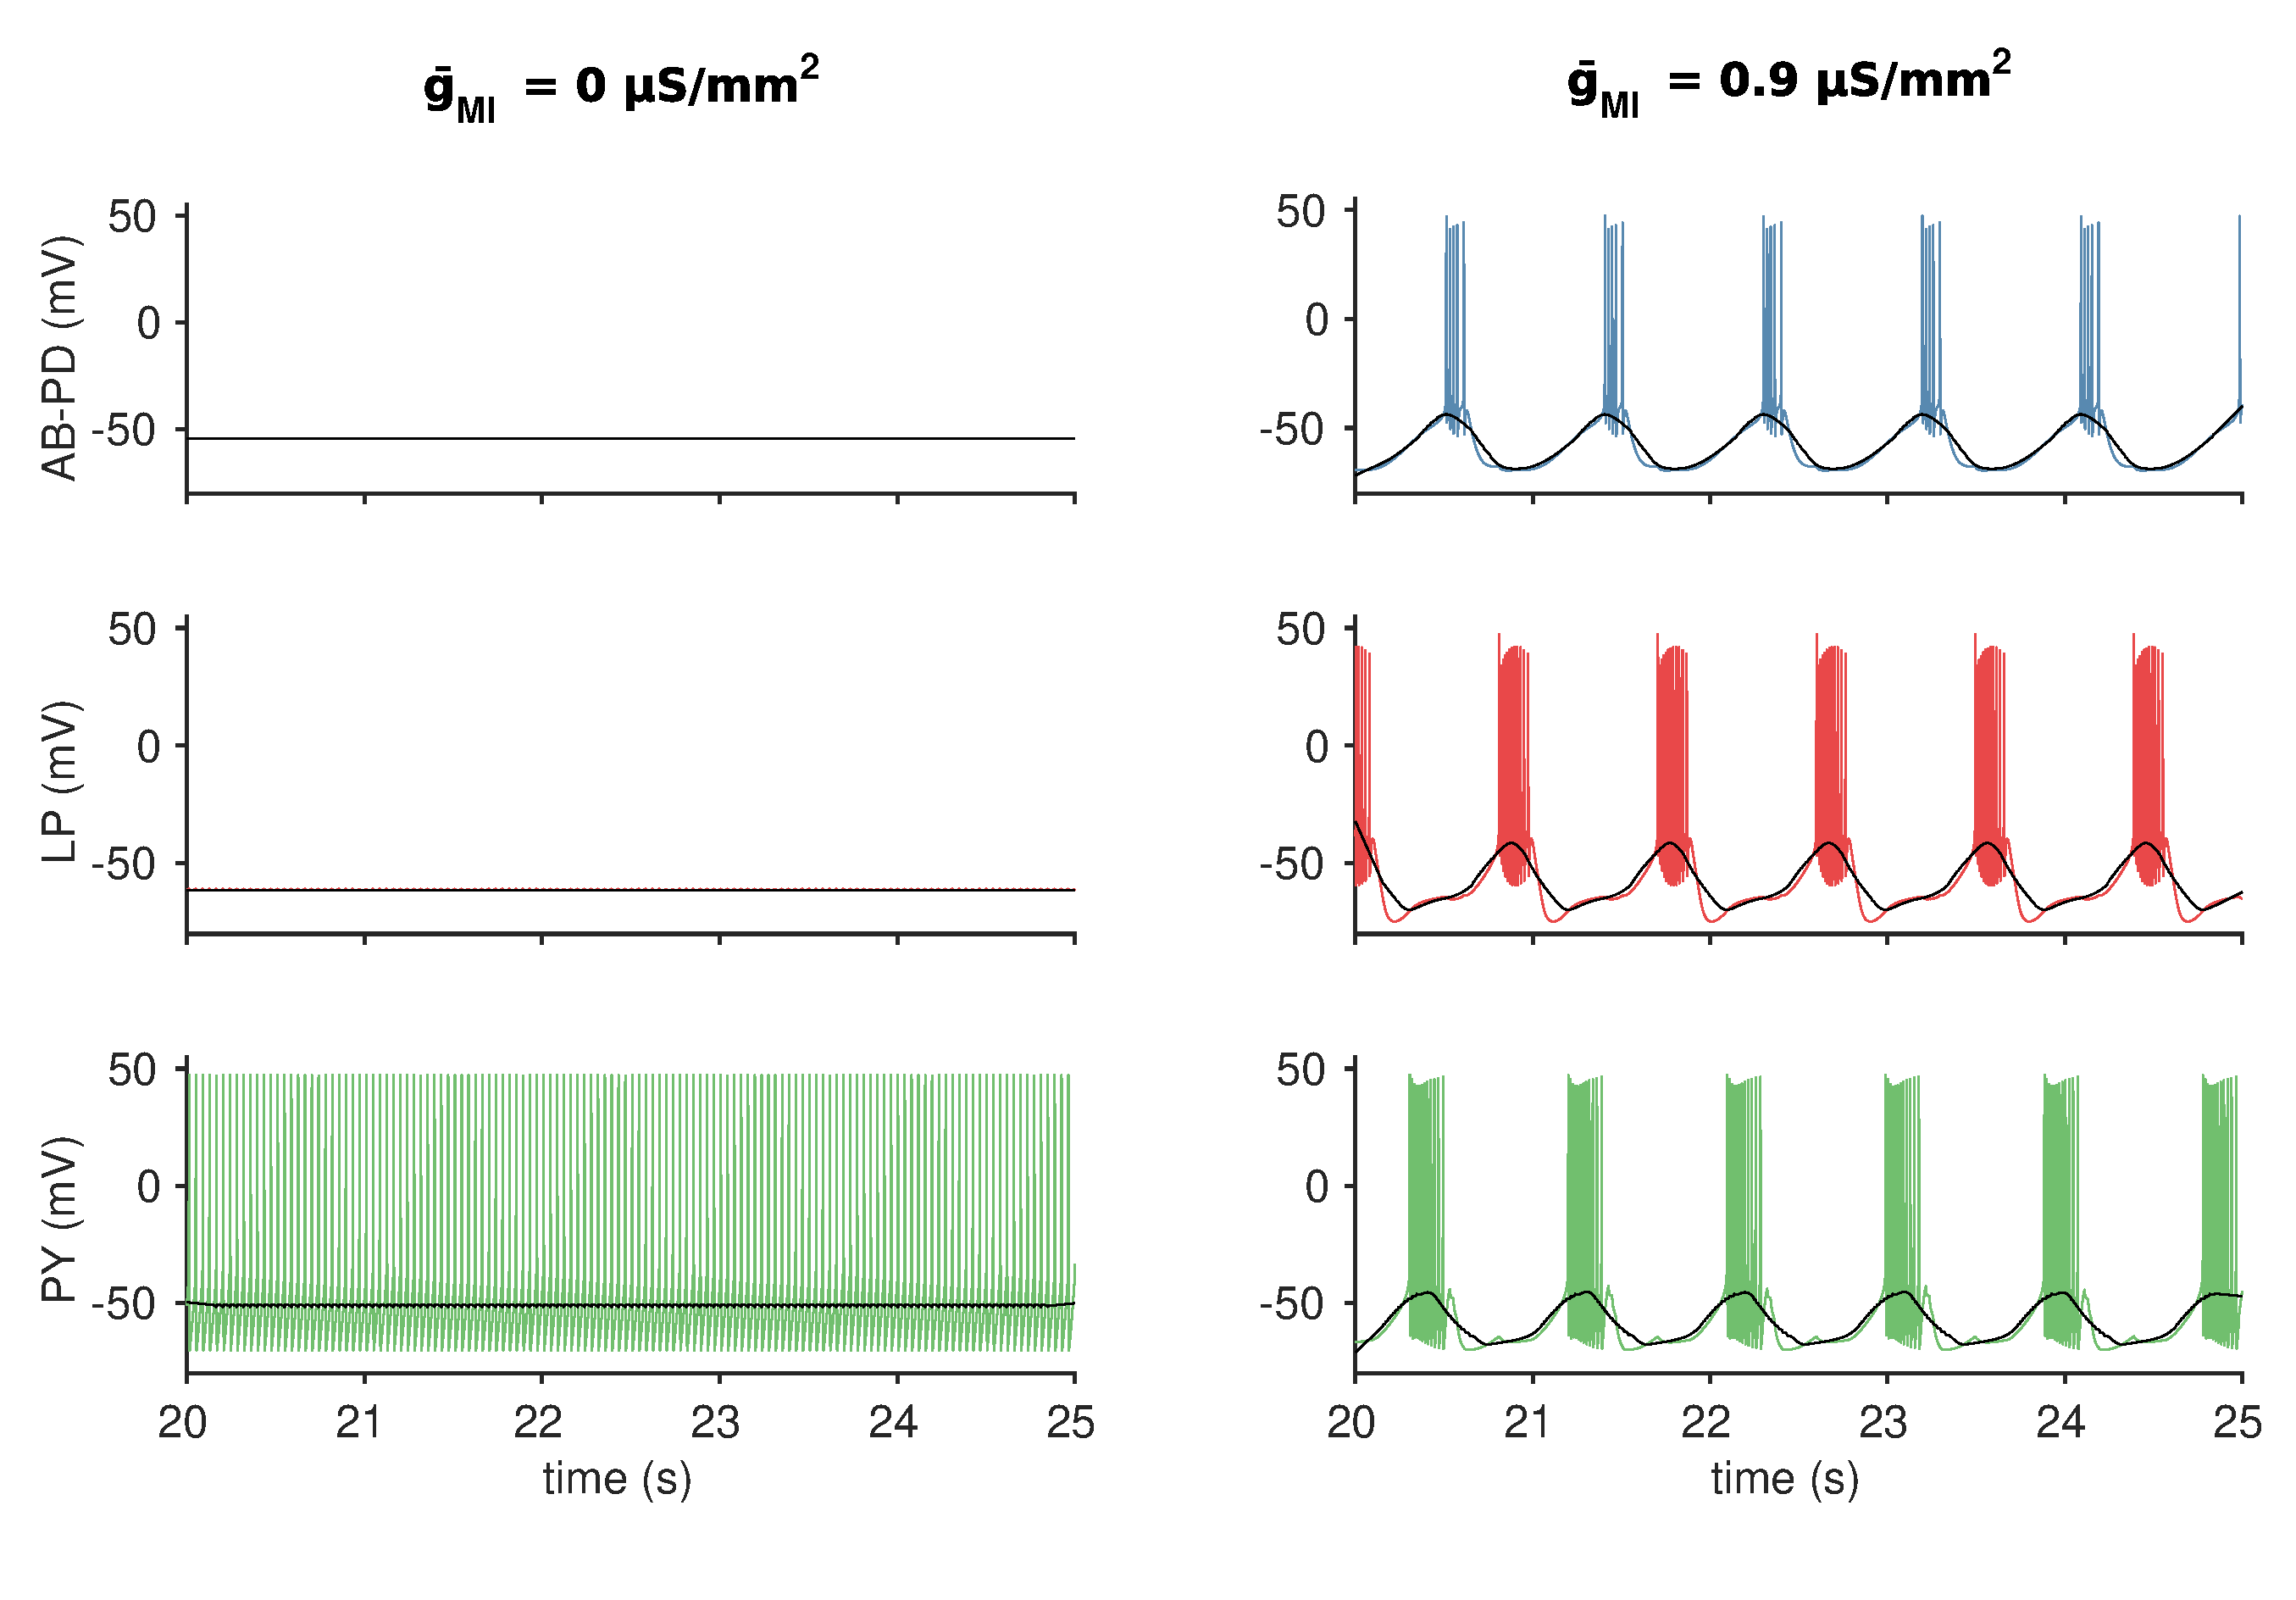
\includegraphics[width=1.0\linewidth]{gfx/network/network_AB_LP_14_traces}
	\caption[Network with modulation into AB-PD \& LP (traces)]{Modulation onto \acs{AB}-\acs{PD} produces triphasic network activity in a quiescent network model. Modulation of the pacemaker increases burst frequency and \acs{AB}-\acs{PD} slow wave amplitude. Left-hand traces are without neuromodulation.. Right-hand traces have \acs{IMI} in \acs{AB}-\acs{PD} at $\bar{g}_{MI} = 0.9~\mu \mathrm{S/mm^2}$. Colors indicate cells (blue is \acs{AB}-\acs{PD}, red is \acs{LP}, green is \acs{PY} and overlaid black indicates the slow wave).}
	\label{fig:networkablp14traces}
\end{figure}

\begin{figure}[h]
	\centering
	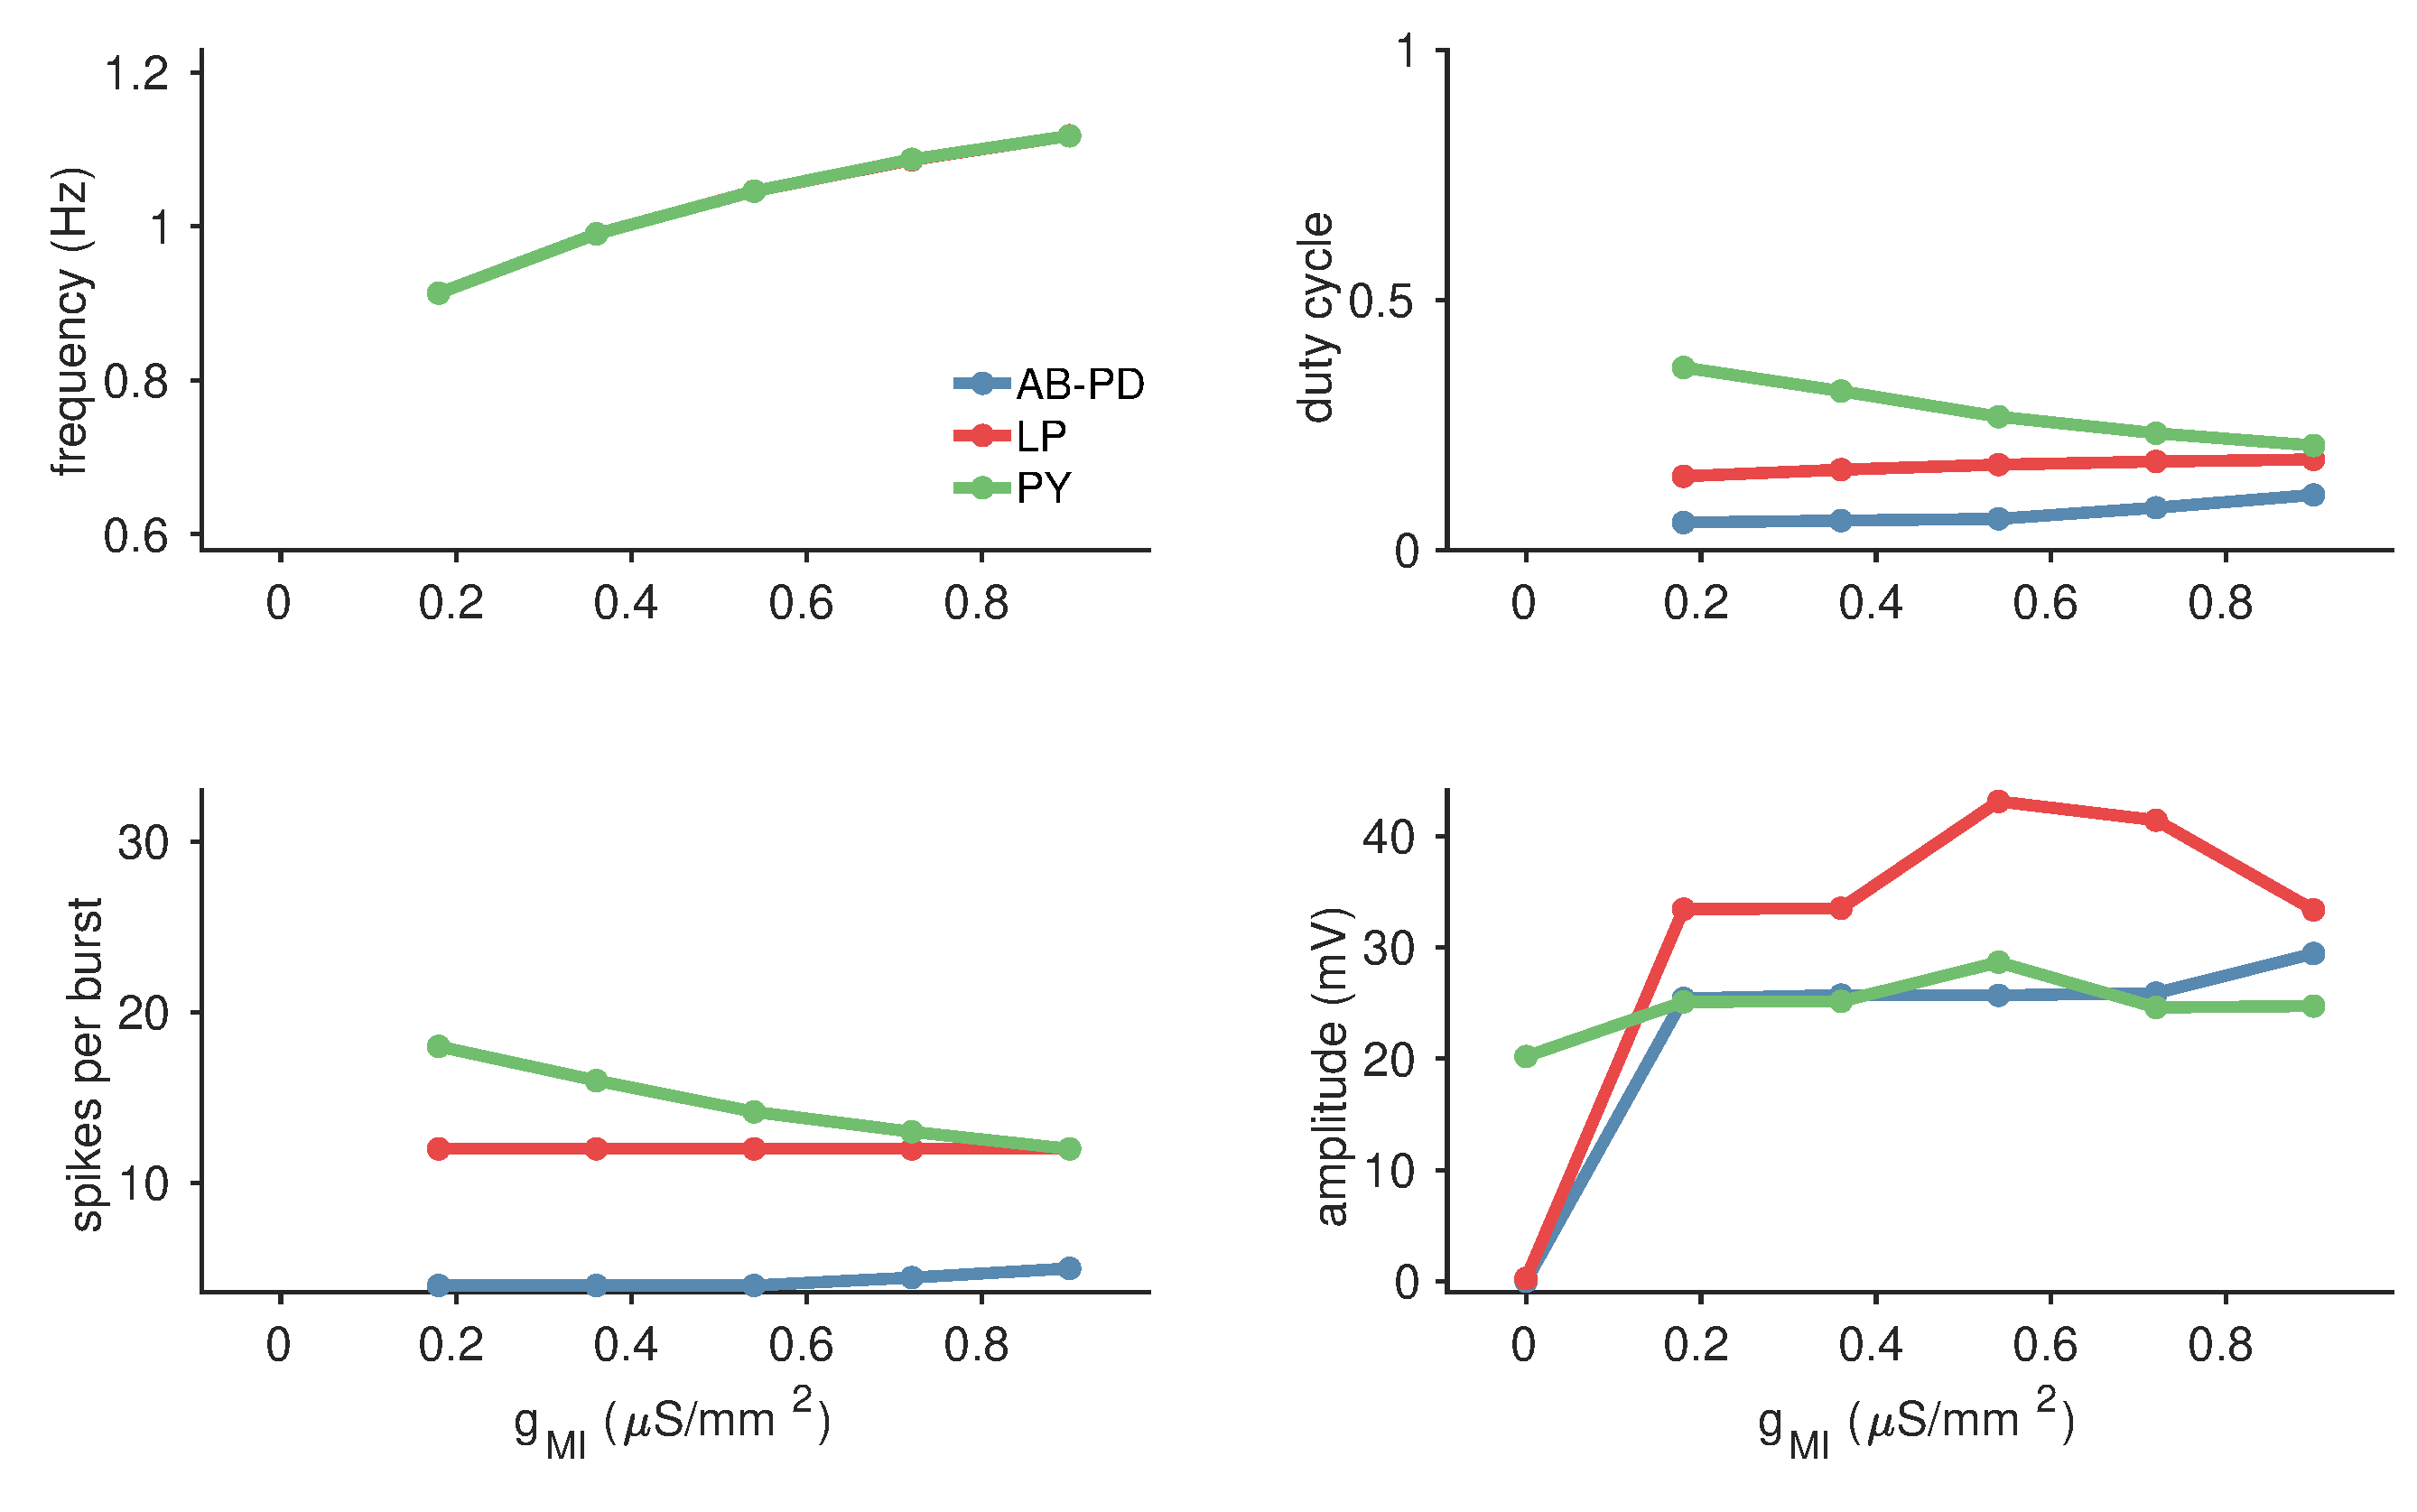
\includegraphics[width=1.0\linewidth]{gfx/network/network_AB_LP_14_metrics}
	\caption[Network with modulation into AB-PD \& LP (metrics)]{Modulation onto \acs{AB}-\acs{PD} produces triphasic network activity in a quiescent network model. Modulation of the pacemaker increases burst frequency and \acs{AB}-\acs{PD} slow wave amplitude. Metrics at steady-state as a function of increasing modulatory input. Colors indicate cells (blue is \acs{AB}-\acs{PD}, red is \acs{LP}, green is \acs{PY}).}
	\label{fig:networkablp14metrics}
\end{figure}

\FloatBarrier

\autoref{fig:networkablp14traces} shows quiescence in the decentralized state and normal triphasic activity with modulation in both the pacemaker and \acs{LP}. Monotonic increase in burst frequency and decrease in duty cycle for models above 0.3 can be seen here as well.

These models qualitatively reproduce slower, variable rhythms in decentralized preparations that recover with activation of \acs{IMI} in \acs{AB}, \acs{PD}, or \acs{LP}.

\FloatBarrier

\subsection{Modulation of AB-PD and LP Promotes Robust Pyloric Rhythms}

Modulatory input conductance was applied to \acs{AB}-\acs{PD} and \acs{LP} model neurons separately and together at differing strengths. Of the 146 models examined, 87 were optimized for pacemaker modulation, 29 for \acs{LP} modulation, and 30 for \acs{IMI} in \acs{AB}-\acs{PD} and \acs{LP}. When models which were triphasic during decentralization were removed, more networks recovered pyloric rhythmicity under modulation of the pacemaker and \acs{LP} than the pacemaker or \acs{LP} alone (\autoref{fig:allstats}).



\begin{figure}
	\centering
	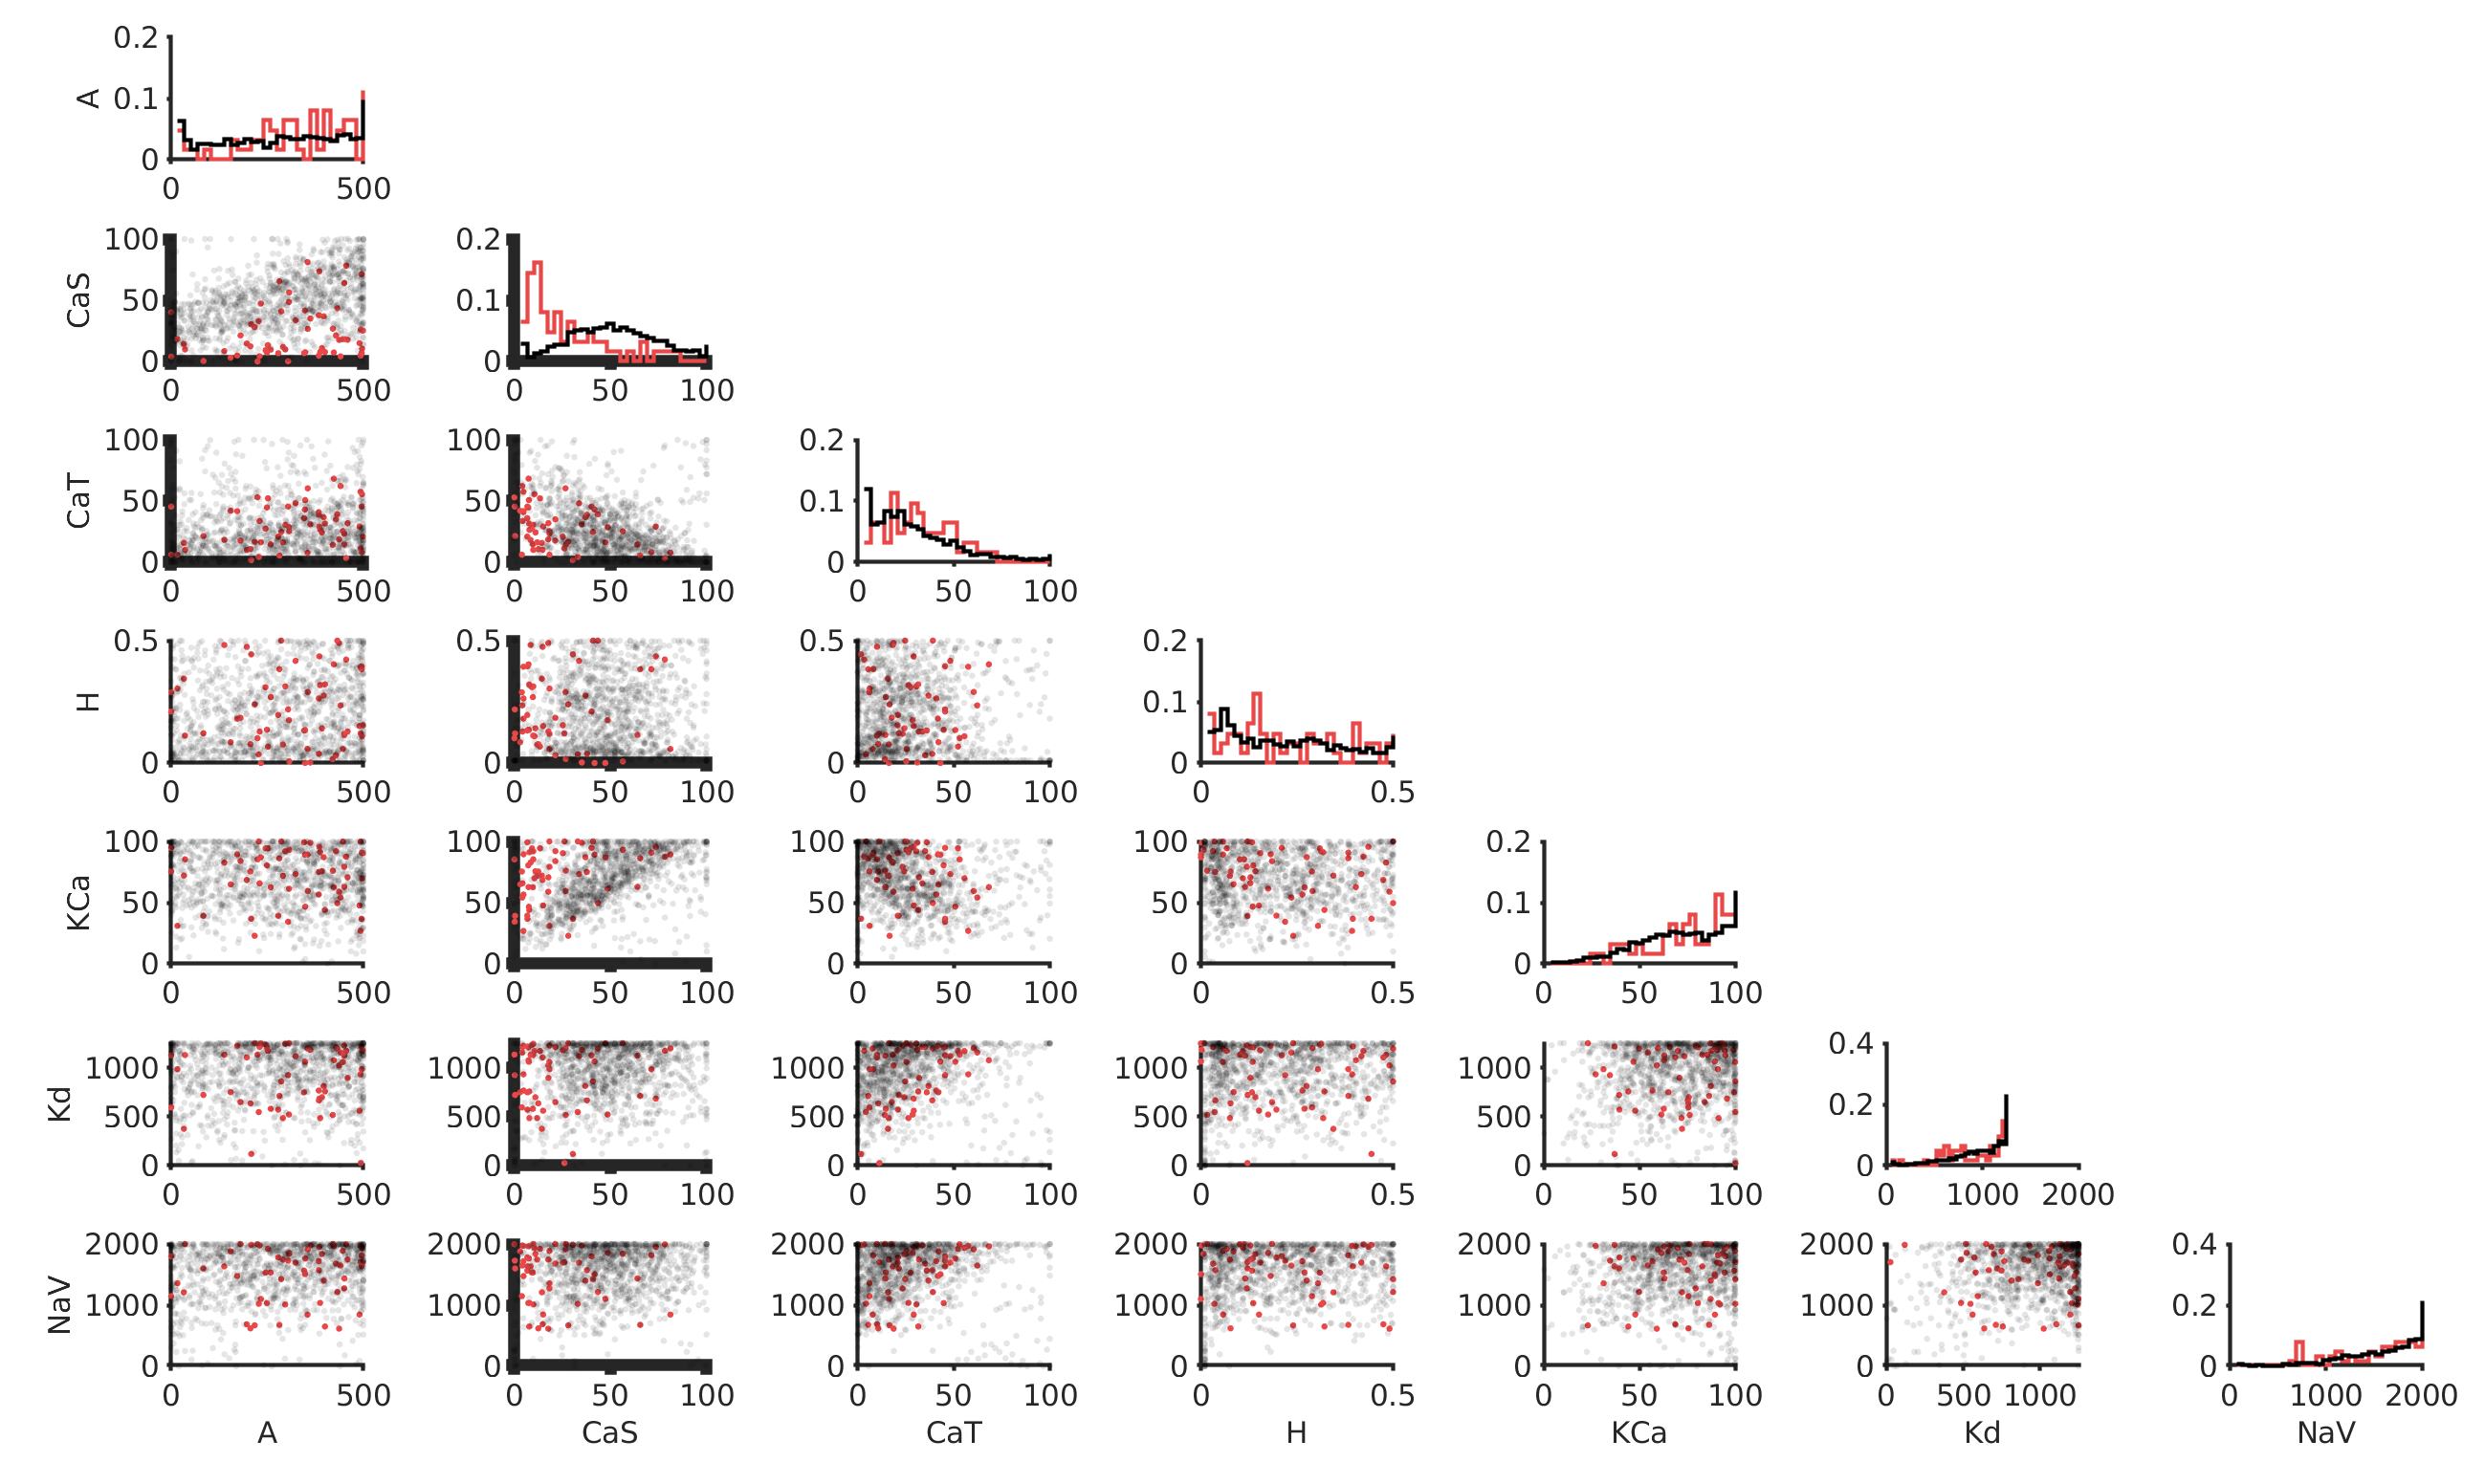
\includegraphics[width=1.3\linewidth]{gfx/all-modulation/correlations_AB}
	\caption[Cross-correlations in AB-PD model maximal conductances]{Cross-correlation in \acs{AB}-\acs{PD} maximal conductances from network models. Maximal conductances from control networks (black, $n=1,148$), which are pyloric in decentralized conditions, and optimized models (red, $n=82$), which are non-pyloric in decentralized conditions and pyloric under modulation onto \acs{AB}-\acs{PD} and \acs{LP}, are plotted against each other. Plots on the diagonal are histograms of maximal conductance. normalized to population size in each case. \textbf{Bold} axes indicate significant correlation (Kolmogorov-Smirnov 2-tailed 2-D test, $p<0.05$). All conductances are in $\mu\mathrm{S/mm^2}.$}  
	\label{fig:correlationsab}
\end{figure}

\begin{figure}
	\centering
	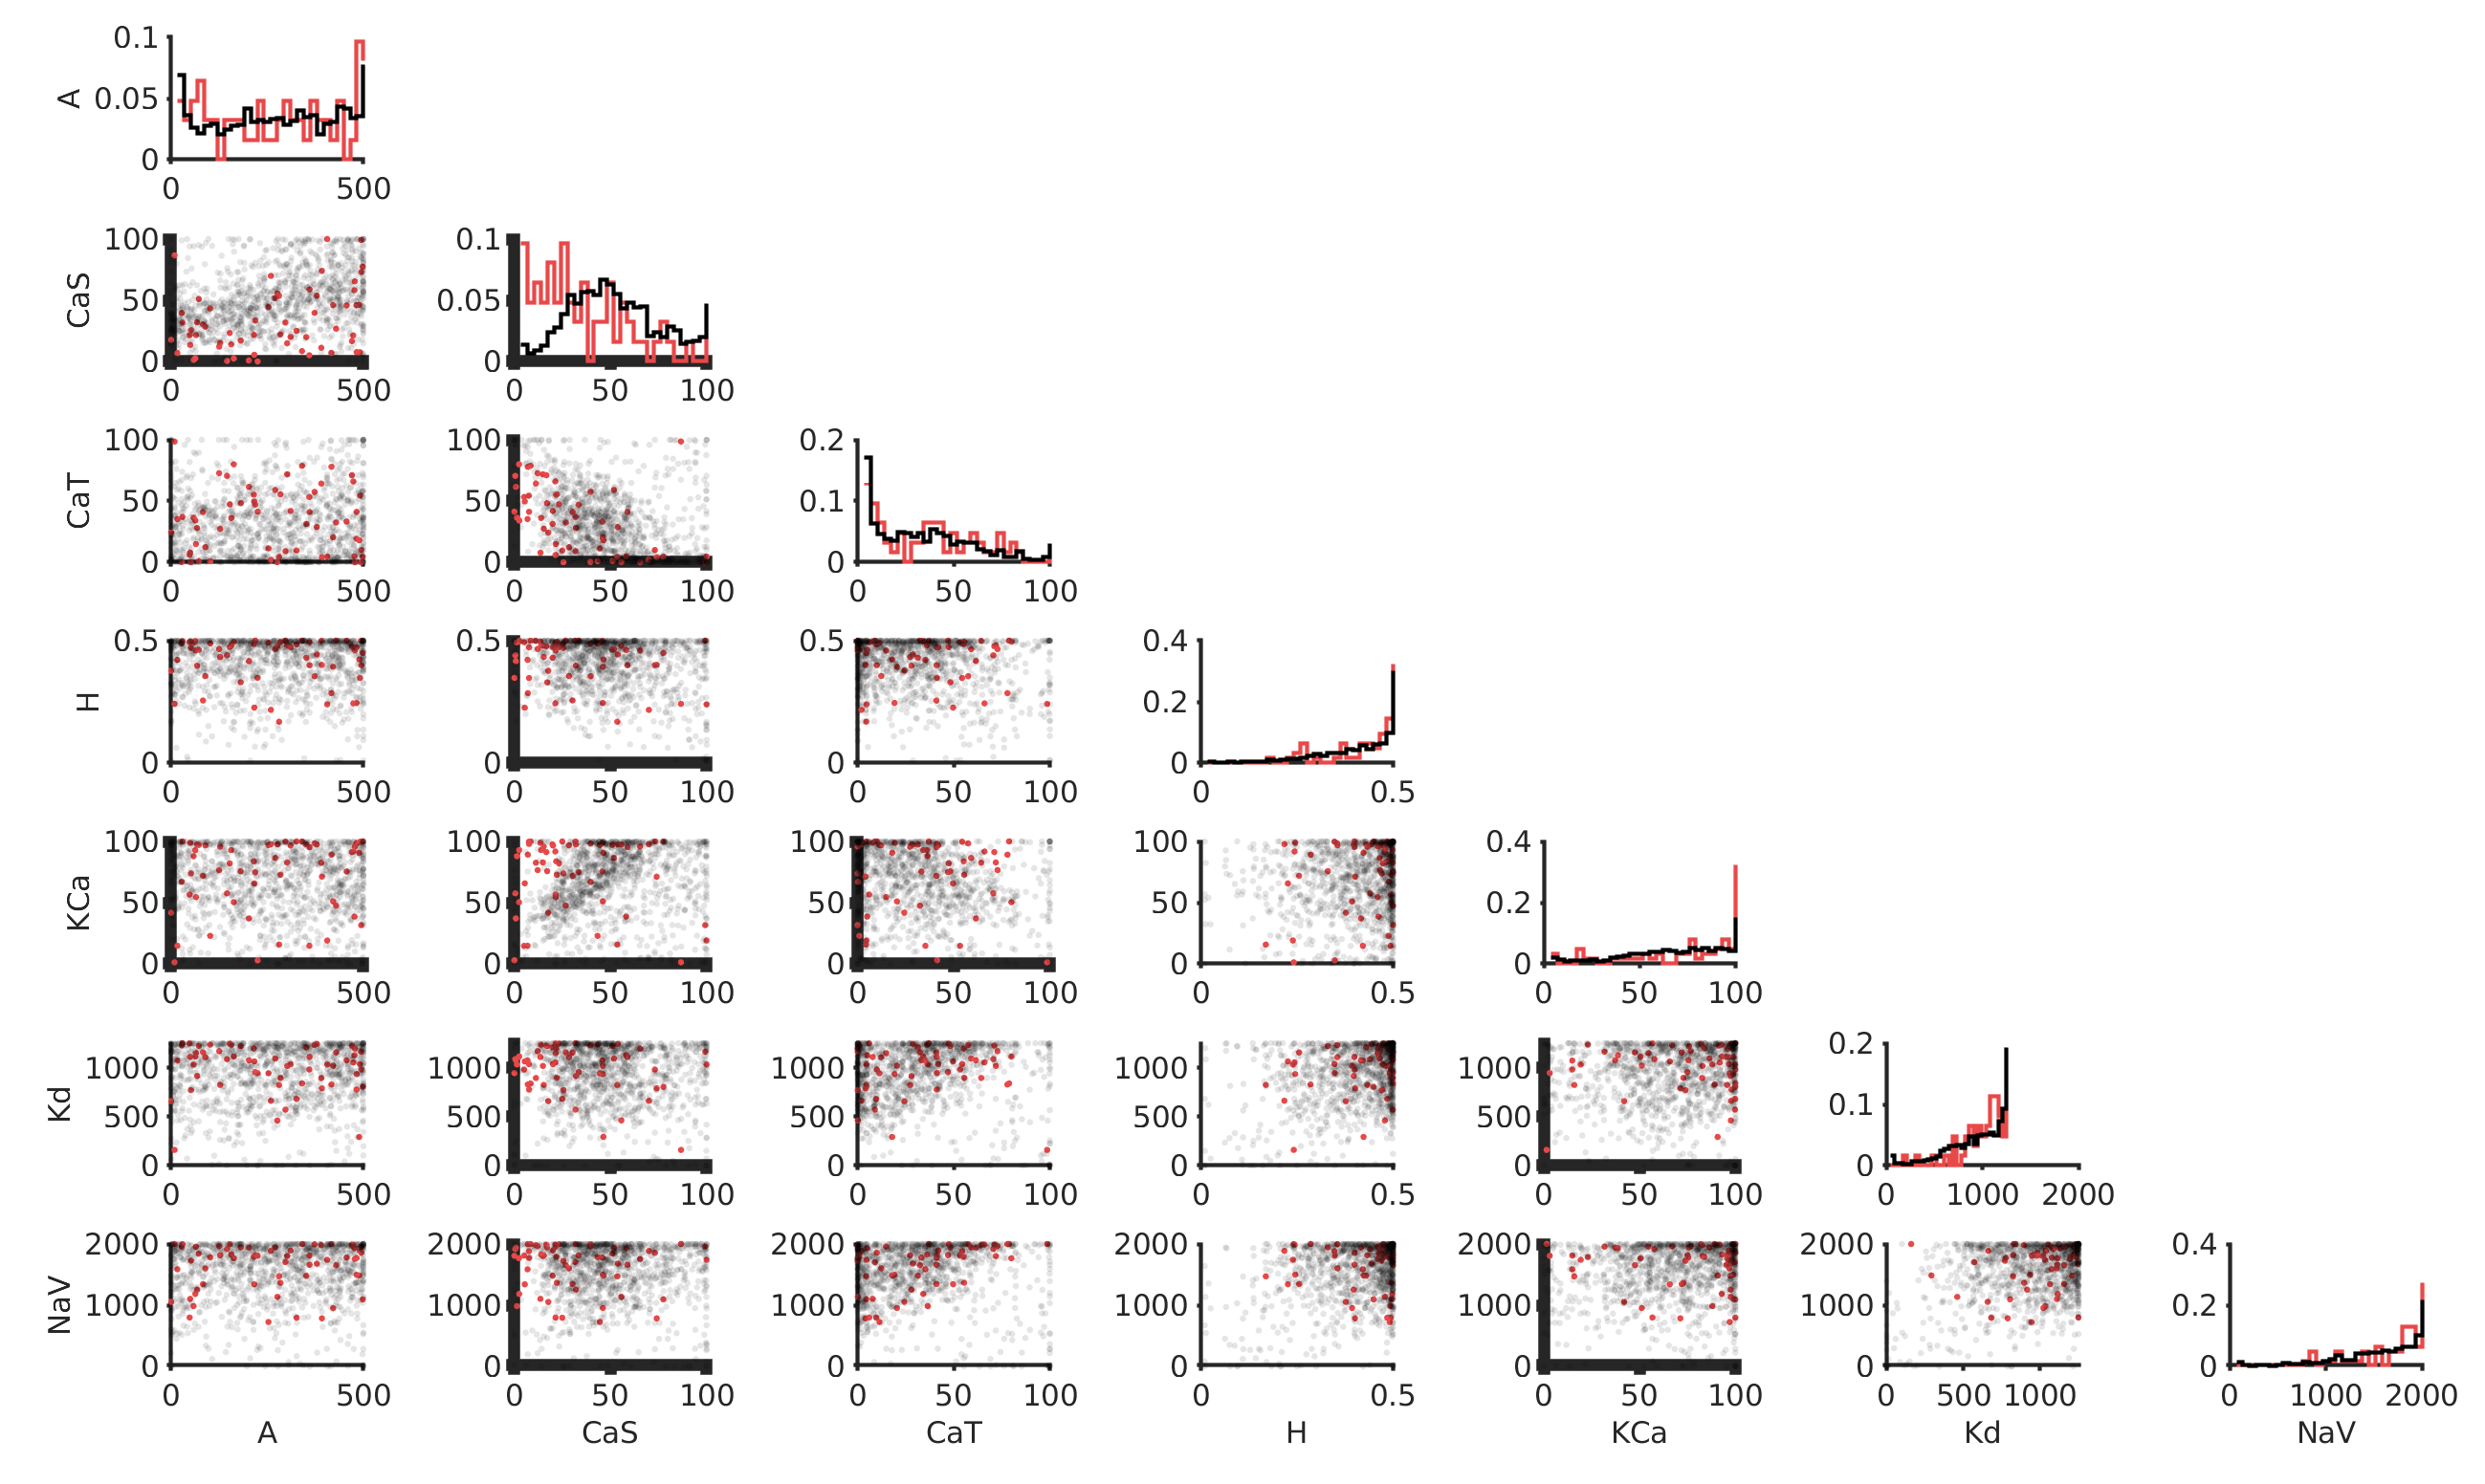
\includegraphics[width=1.3\linewidth]{gfx/all-modulation/correlations_LP}
	\caption[Cross-correlations in LP model maximal conductances]{Cross-correlation in \acs{LP} maximal conductances from network models. Maximal conductances from control networks (black, $n=1,148$), which are pyloric in decentralized conditions, and optimized models (red, $n=82$), which are non-pyloric in decentralized conditions and pyloric under modulation onto \acs{AB}-\acs{PD} and \acs{LP}, are plotted against each other. Plots on the diagonal are histograms of maximal conductance. normalized to population size in each case. \textbf{Bold} axes indicate significant correlation (Kolmogorov-Smirnov 2-tailed 2-D test, $p<0.05$). All conductances are in $\mu\mathrm{S/mm^2}.$}  
	\label{fig:correlationslp}
\end{figure}

\begin{figure}
	\centering
	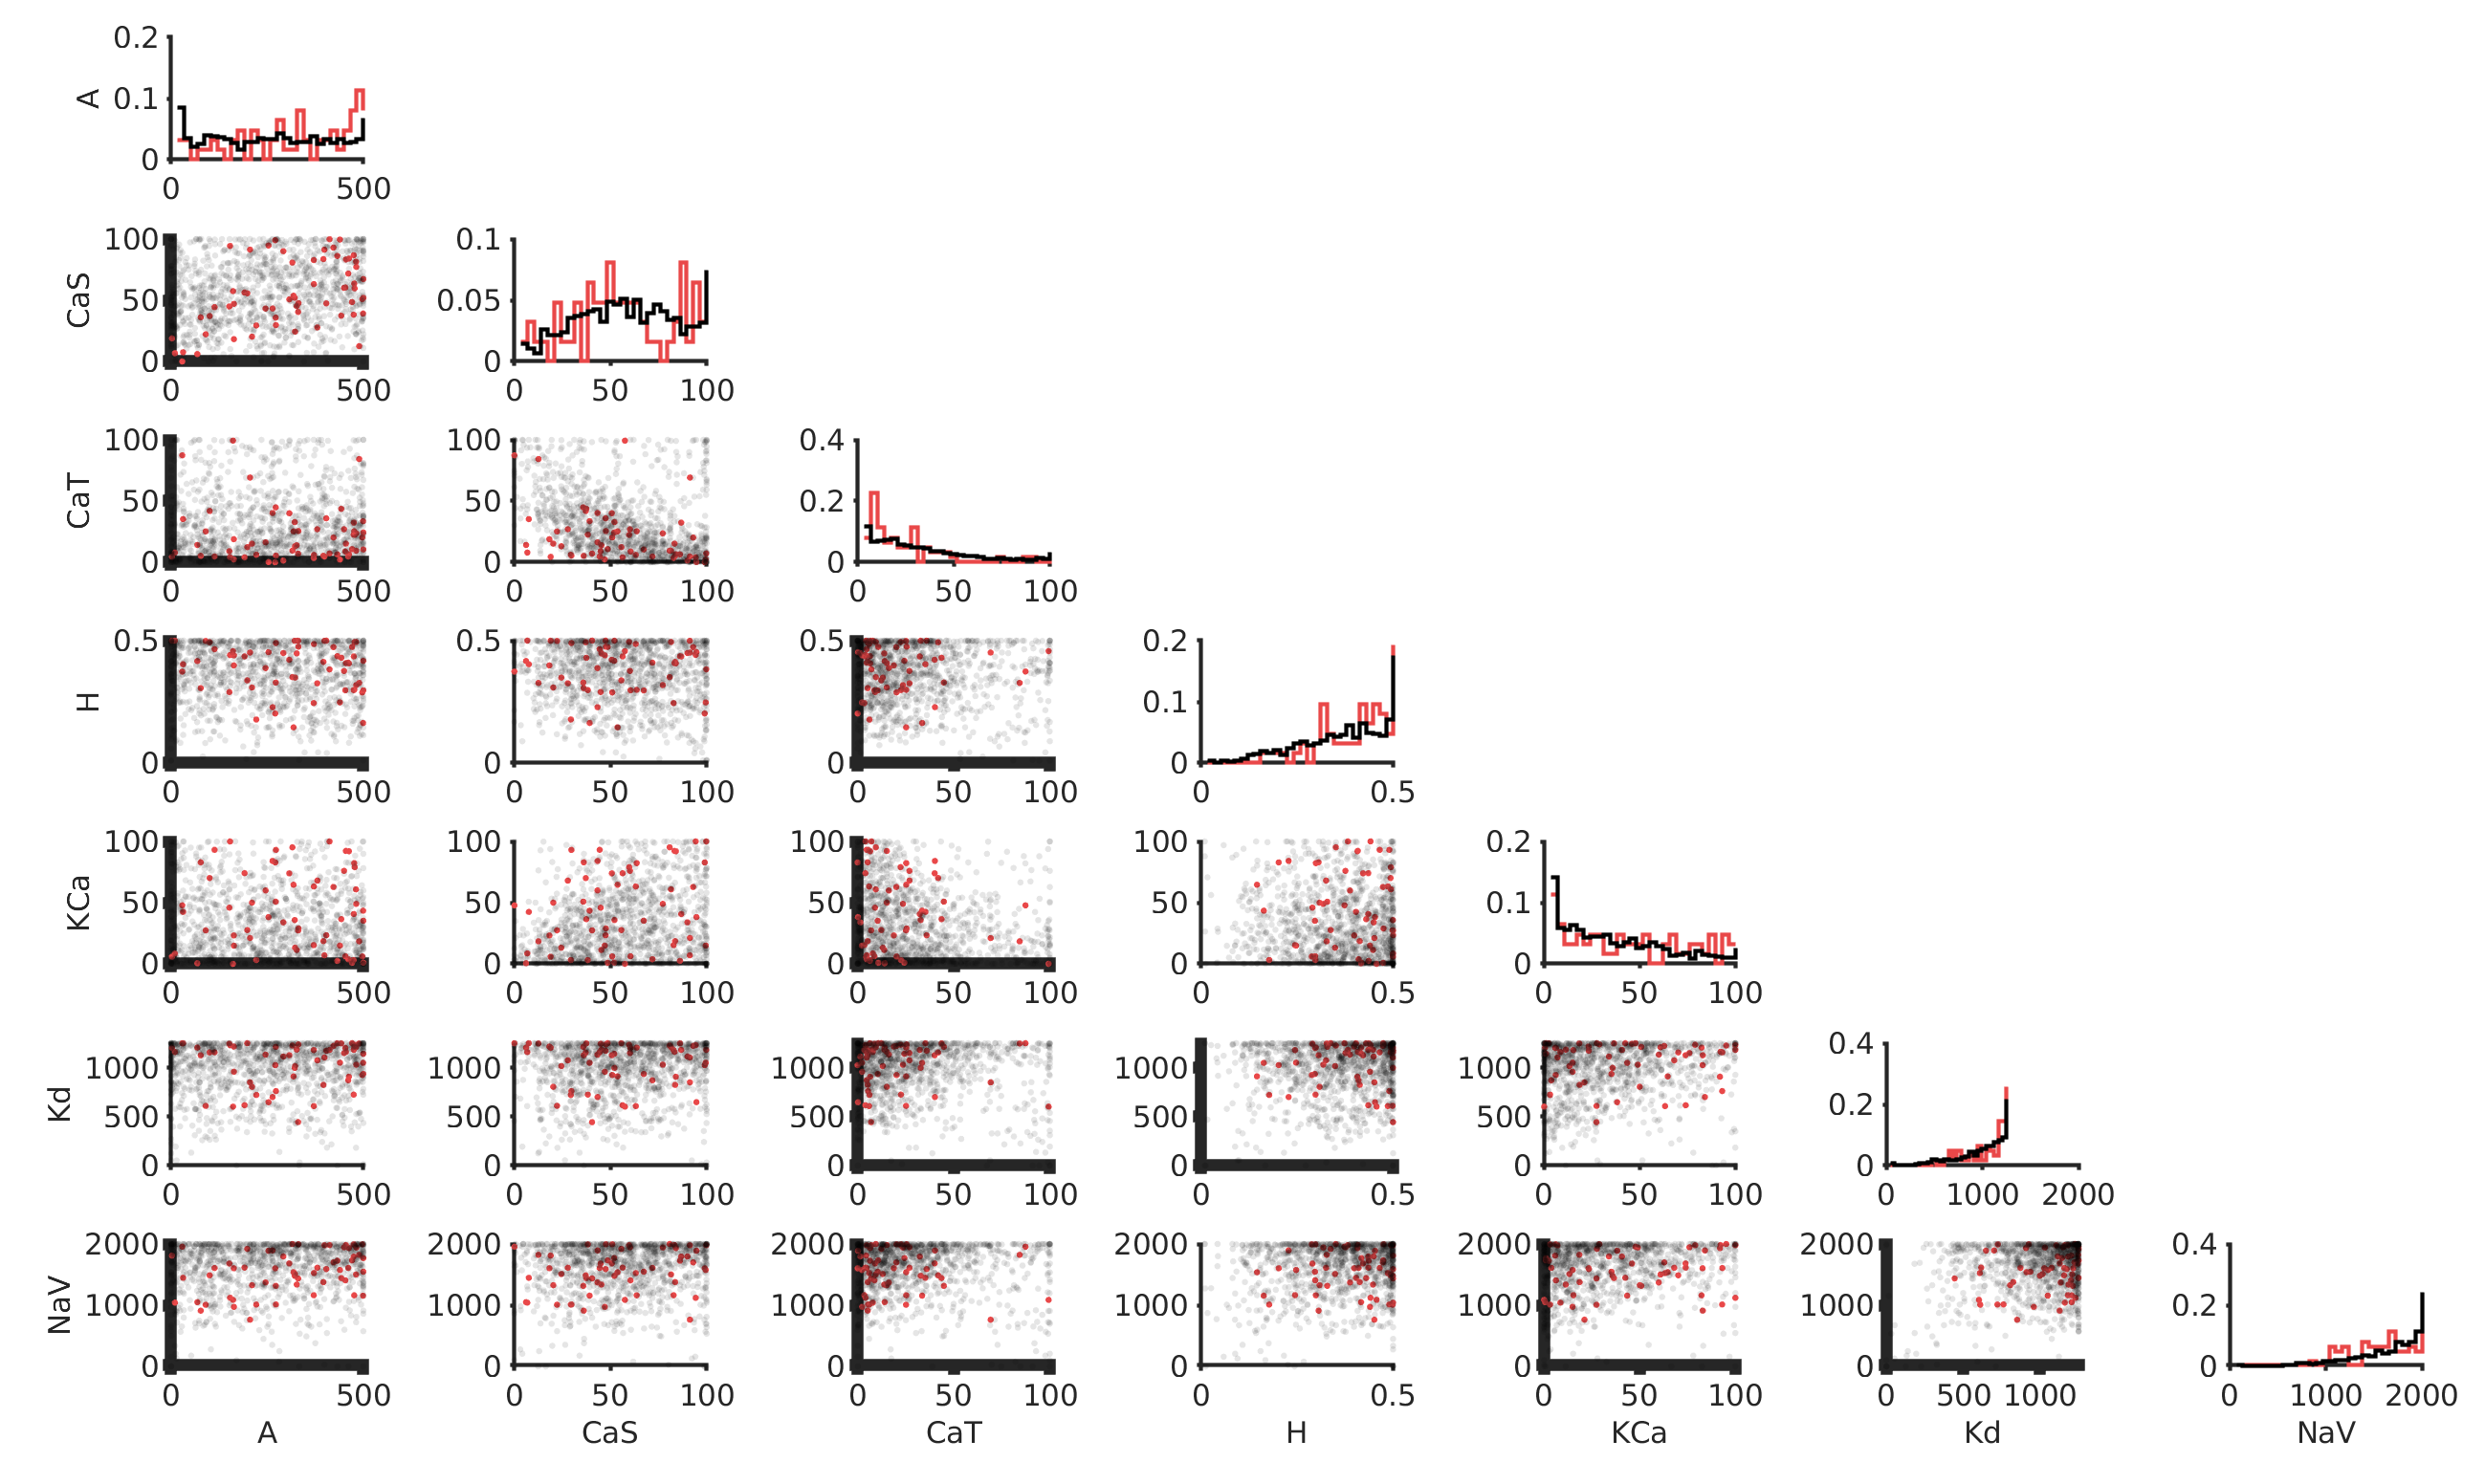
\includegraphics[width=1.3\linewidth]{gfx/all-modulation/correlations_PY}
	\caption[Cross-correlations in PY model maximal conductances]{Cross-correlation in \acs{PY} maximal conductances from network models. Maximal conductances from control networks (black, $n=1,148$), which are pyloric in decentralized conditions, and optimized models (red, $n=82$), which are non-pyloric in decentralized conditions and pyloric under modulation onto \acs{AB}-\acs{PD} and \acs{LP}, are plotted against each other. Plots on the diagonal are histograms of maximal conductance. normalized to population size in each case. \textbf{Bold} axes indicate significant correlation (Kolmogorov-Smirnov 2-tailed 2-D test, $p<0.05$). All conductances are in $\mu\mathrm{S/mm^2}.$}  
	\label{fig:correlationspy}
\end{figure}

\begin{figure}
	\centering
	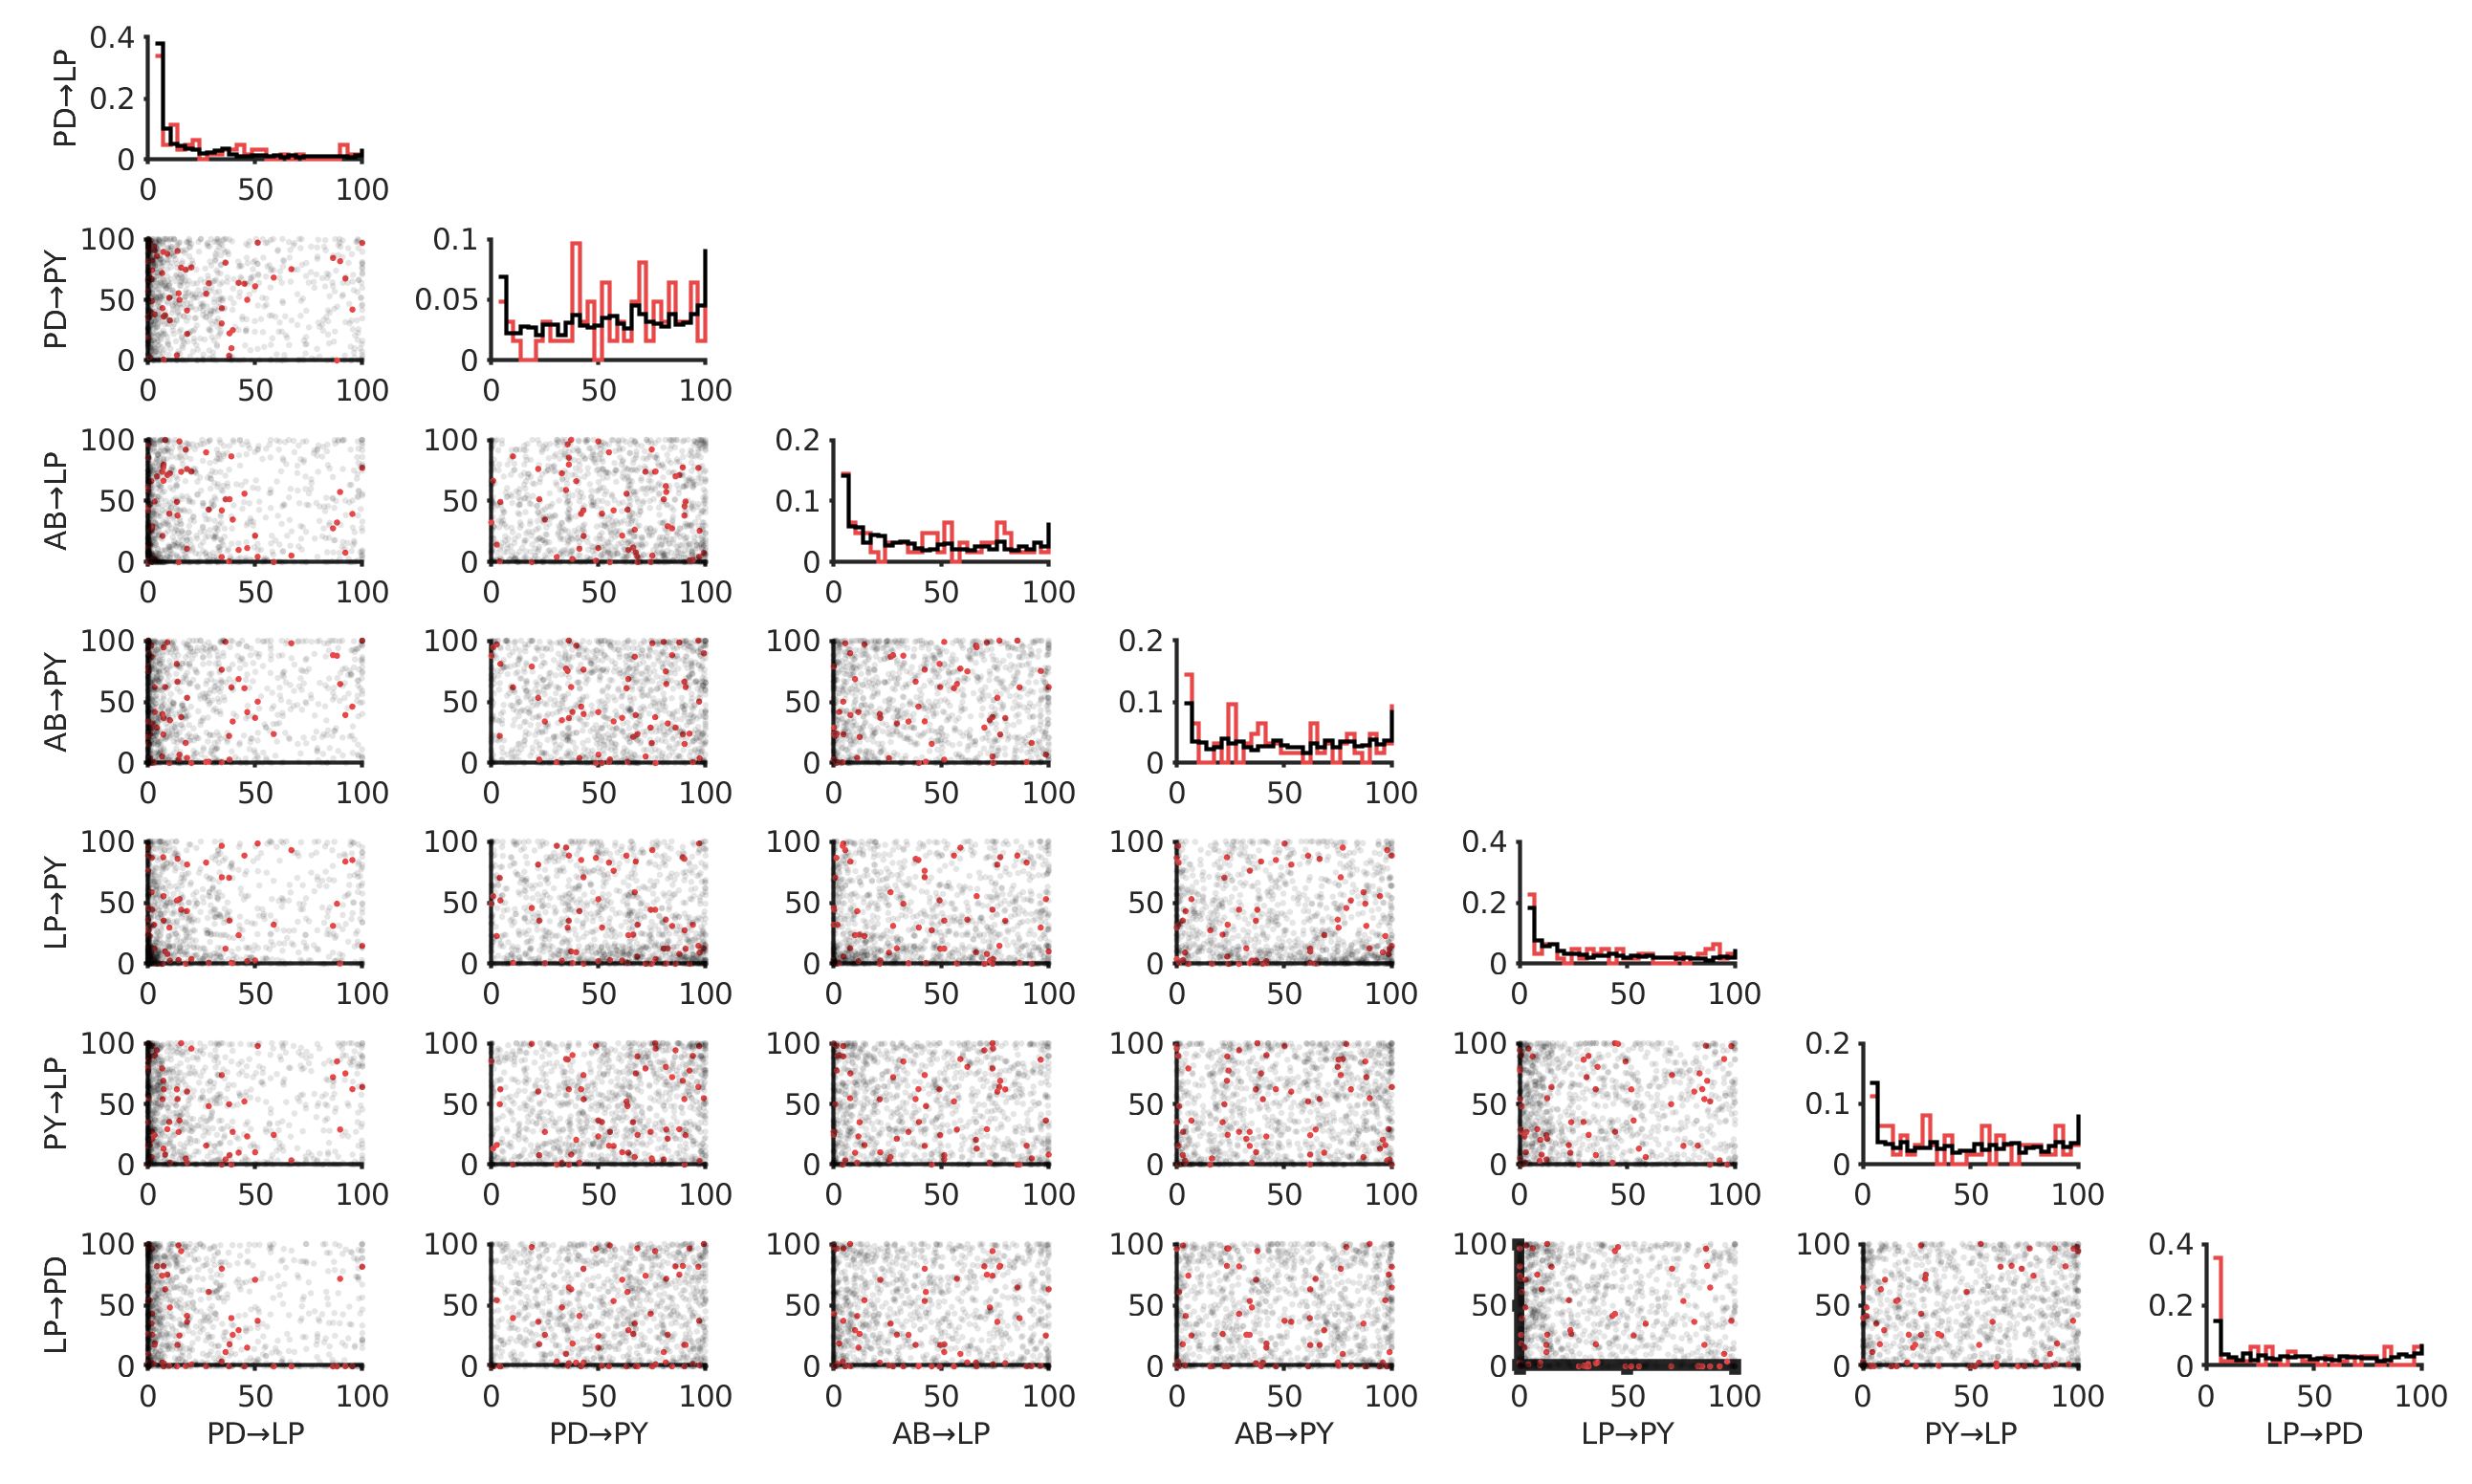
\includegraphics[width=1.3\linewidth]{gfx/all-modulation/correlations_synapses}
	\caption[Cross-correlations in synaptic maximal conductances]{Cross-correlation in synaptic maximal conductances from network models. Arrows point from presynaptic to post-synaptic neurons. All synapses are inhibitory and glutamatergic except for synapses from \acs{PD} which are cholinergic. Maximal conductances from control networks (black, $n=1,148$), which are pyloric in decentralized conditions, and optimized models (red, $n=82$), which are non-pyloric in decentralized conditions and pyloric under modulation onto \acs{AB}-\acs{PD} and \acs{LP}, are plotted against each other. Plots on the diagonal are histograms of maximal conductance. normalized to population size in each case. \textbf{Bold} axes indicate significant correlation (Kolmogorov-Smirnov 2-tailed 2-D test, $p<0.05$). All conductances are in $\mu\mathrm{S/mm^2}.$} 
	\label{fig:correlationssynapses}
\end{figure}


We hypothesized that this effect is caused by the effectiveness of post-inhibitory rebound as a mechanism for stabilization of central patterns. \acs{AB}-\acs{PD} and \acs{LP} mutually inhibit each other. Phasic excitation applied to each network component during the rising phase of the slow wave would then drive the network through enhanced mutual inhibition.

\begin{figure}
	\centering
	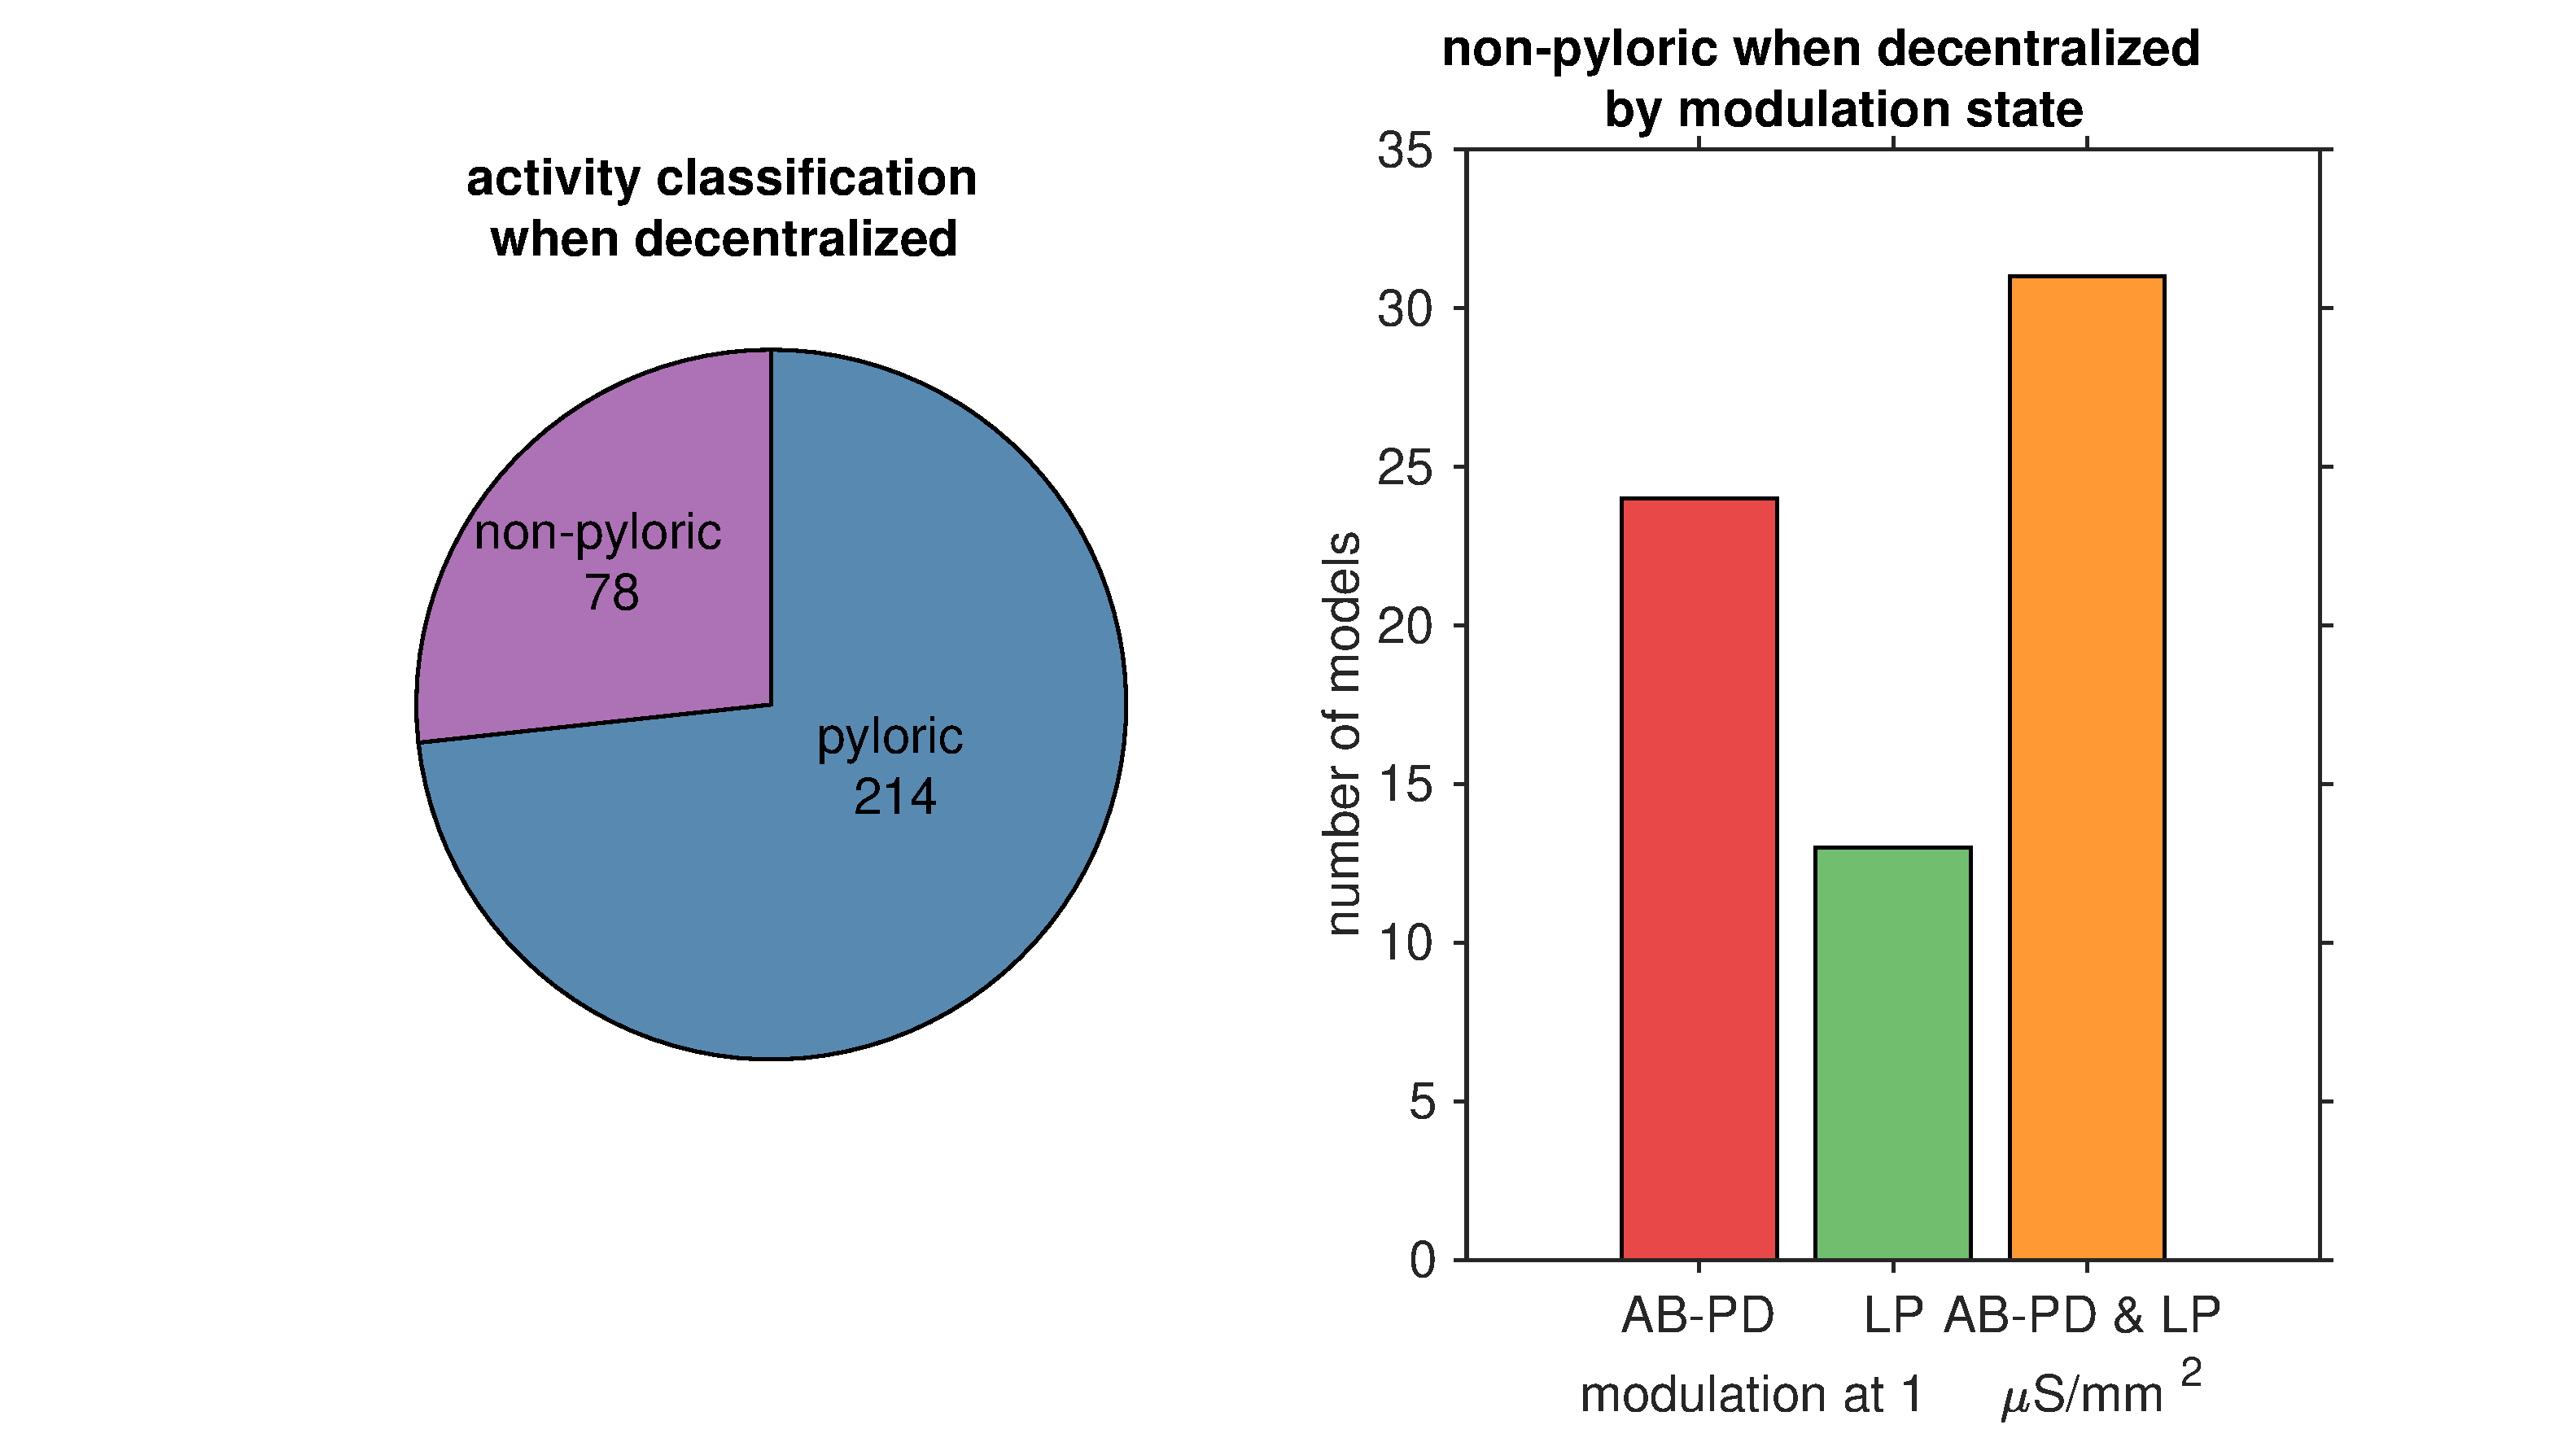
\includegraphics[width=1.0\linewidth]{gfx/all-modulation/all_stats}
	\caption[Distribution of rhythmicity in network models]{Distribution of triphasic network models by modulation state ($n=146$). \textit{Left:} Most triphasic models have \acs{IMI} in the pacemaker kernel and \acs{LP}, representing intact descending modulation, though many optimized models are triphasic in the decentralized state. This is due to optimization selecting for pyloric-like models \textit{prima facie}. \textit{Right:} When models which are triphasic in the decentralized state are excluded, most parameter sets result in triphasic networks with modulation and aberrant networks when decentralized.}
	\label{fig:allstats}
\end{figure}

The role of \acs{AB} and \acsp{PD} as the pacemaker kernel is recapitulated in these models. Modulation onto \acs{AB}-\acs{PD} more strongly drives network activity than modulation onto \acs{LP}. Models were classified as pyloric or non-pyloric in the four cases of modulation (decentralized, \acs{AB}-\acs{PD}, \acs{LP}, both). Correlations between classified network activity in these states reveals strong correlation between \acs{AB}-\acs{PD} and \acs{AB}-\acs{PD} \& \acs{LP} modulation states (\autoref{tab:correlations}).

To identify specific conductances important in models which respond to \acs{IMI}, correlations between maximal conductances from model networks which were non-pyloric in decentralized conditions, and pyloric with \acs{IMI} in \acs{AB}-\acs{PD} and \acs{LP} were computed. The 1,148 pyloric models from which the 146 networks were optimized for response to modulatory input were use as control data (\autoref{sec:parameteroptimization}). Maximal conductances for the three model neurons and seven synapses were plotted in cross-correlation diagrams (\autoref{fig:correlationsab}, \autoref{fig:correlationslp}, \autoref{fig:correlationspy}, \autoref{fig:correlationssynapses}). 

Two-sample, two-tailed two-dimensional Kolmogorov-Smirnov tests were used to determine significance\autocite{PeacockTwodimensionalgoodnessoffittesting1983}. Significant correlations were found between \acs{ICas} and all other conductances ($p < 0.05$) in \acs{AB}-\acs{PD} models. We hypothesize that since slow-wave calcium is responsible for burst propagation, models with low slow-calcium conductance are more responsive to neuromodulation in the form of \acs{IMI}, an inward current which activates near the peak of the slow wave. \acs{LP} model neurons also show reduced slow-wave calcium maximal conductance in comparison to the control networks. In addition, low \acs{ICaS} co-occurs with high \acs{IKCa} and \acs{IH}. \acs{IKCa} activates during burst termination and \acs{IH} rectifies hyperpolarization. Strong after-burst hyperpolarization, coupled with modulation- and \acs{IH}-mediated recovery would explain the increase in burst frequency and amplitude seen with \acs{IMI} activation. In \acs{PY}, higher \acs{ICaS},  \acs{IH}, and \acs{LP} to \acs{PY} inhibitory synapse maximal conductances indicate strong excitability with post-inhibitory rebound. \acs{PY} is not modulated by \acs{RPCH} and must burst in response to inhibitory synaptic feedback. 

\begin{table}[h]
	\myfloatalign
	\begin{tabularx}{\textwidth}{ccccc} \toprule
		& \tableheadline{dec.} & \tableheadline{AB-PD} & \tableheadline{LP} & \tableheadline{AB-PD \& LP} \\ \midrule
		\tableheadline{dec.} & 1 & 0.1986 & 0.4773 & 0.1990 \\
		\tableheadline{AB-PD} & 0.1986 & 1 & 0.0600 & 0.6751 \\
		\tableheadline{LP} & 0.4773 & 0.0600 &  1 & 0.09702 \\
		\tableheadline{AB-PD \& LP} & 0.1990 & 0.6751 & 0.09702 & 1 \\
		\bottomrule
	\end{tabularx}
	\caption[Correlation between pyloric activity in different modulation states]{Correlation between models under modulation regimes classified as pyloric or non-pyloric demonstrates the role of the \acs{AB}-\acs{PD} composite as pacemaker kernel. Modulation into \acs{AB}-\acs{PD} and \acs{AB}-\acs{PD} \& \acs{LP} is most strongly correlated. \acs{AB}-\acs{PD} is responsive to modulatory input and drives the circuit rhythm.}  
	\label{tab:correlations}
\end{table}

\begin{figure}
	\centering
	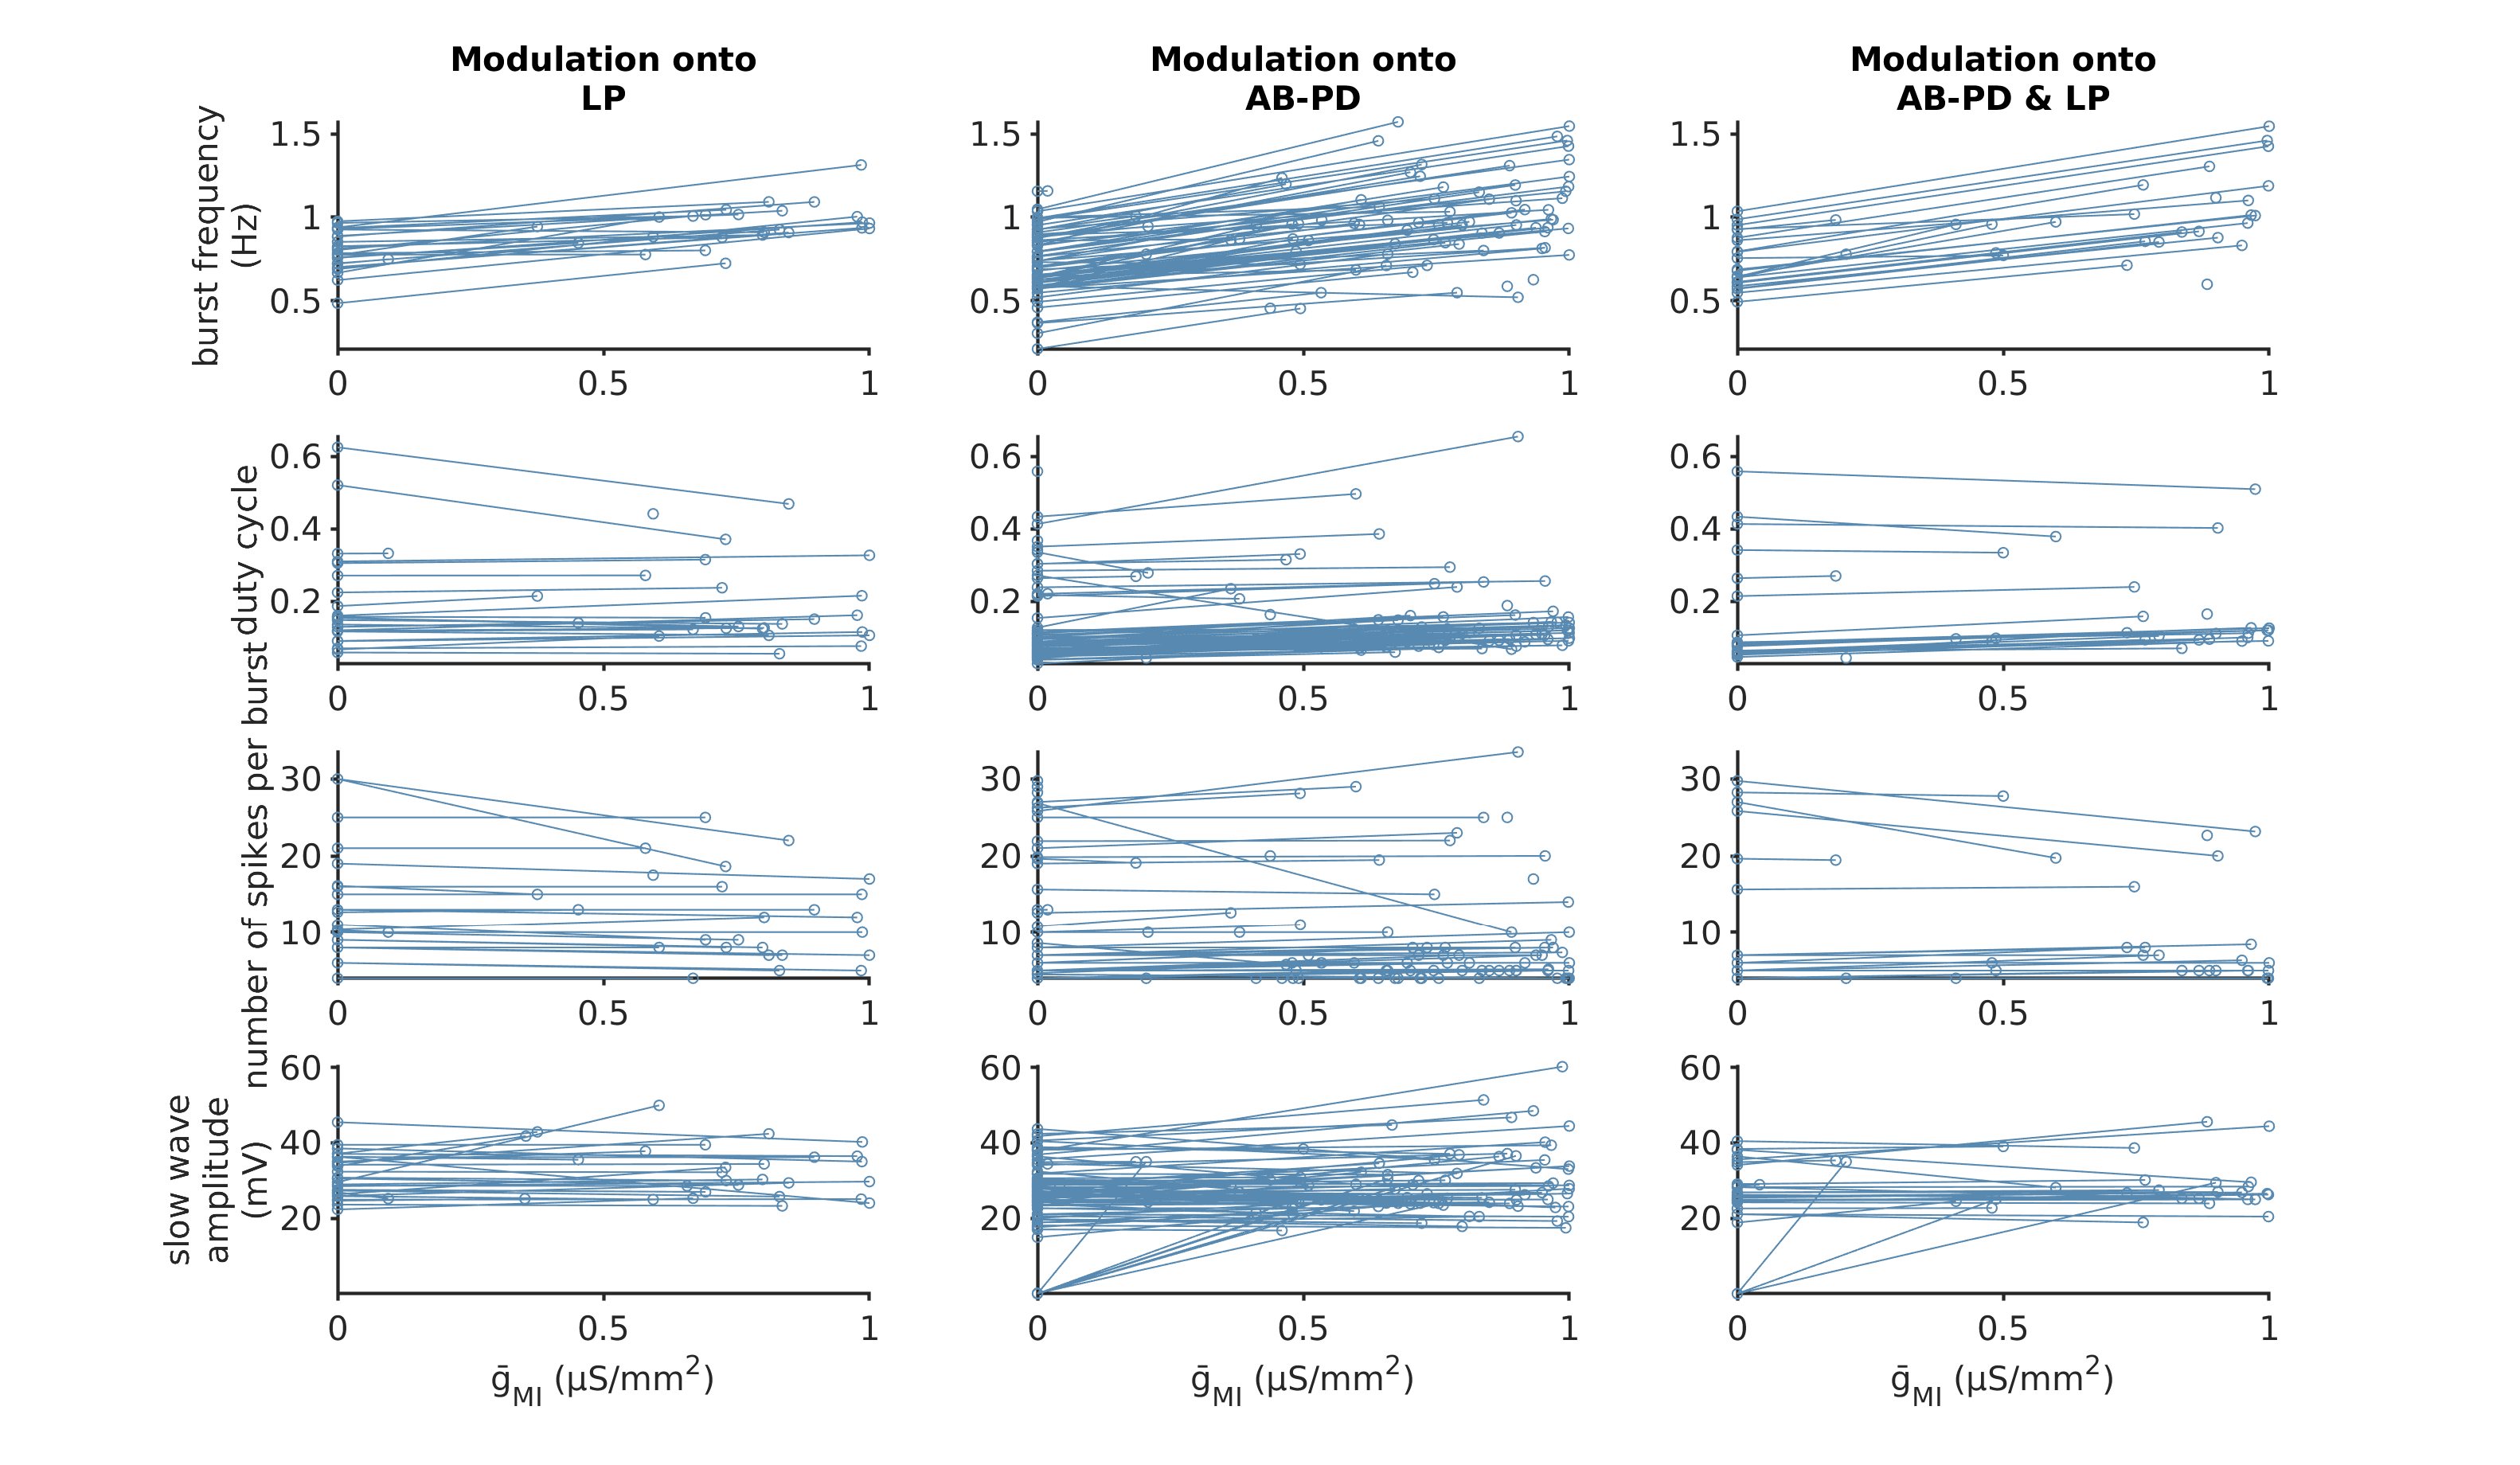
\includegraphics[width=1.0\linewidth]{gfx/all-modulation/metrics_AB}
	\caption[All optimized ABPD models in decentralized and modulated cases]{146 network models in decentralized and modulated cases show increased burst frequency and amplitude under modulated conditions with respect to decentralization. Modulation under \acs{AB}-\acs{PD} and \acs{LP} produces the most regular triphasic output. Colors indicate cells (blue is \acs{AB}-\acs{PD}).}
	\label{fig:metricsab}
\end{figure}

\begin{figure}
	\centering
	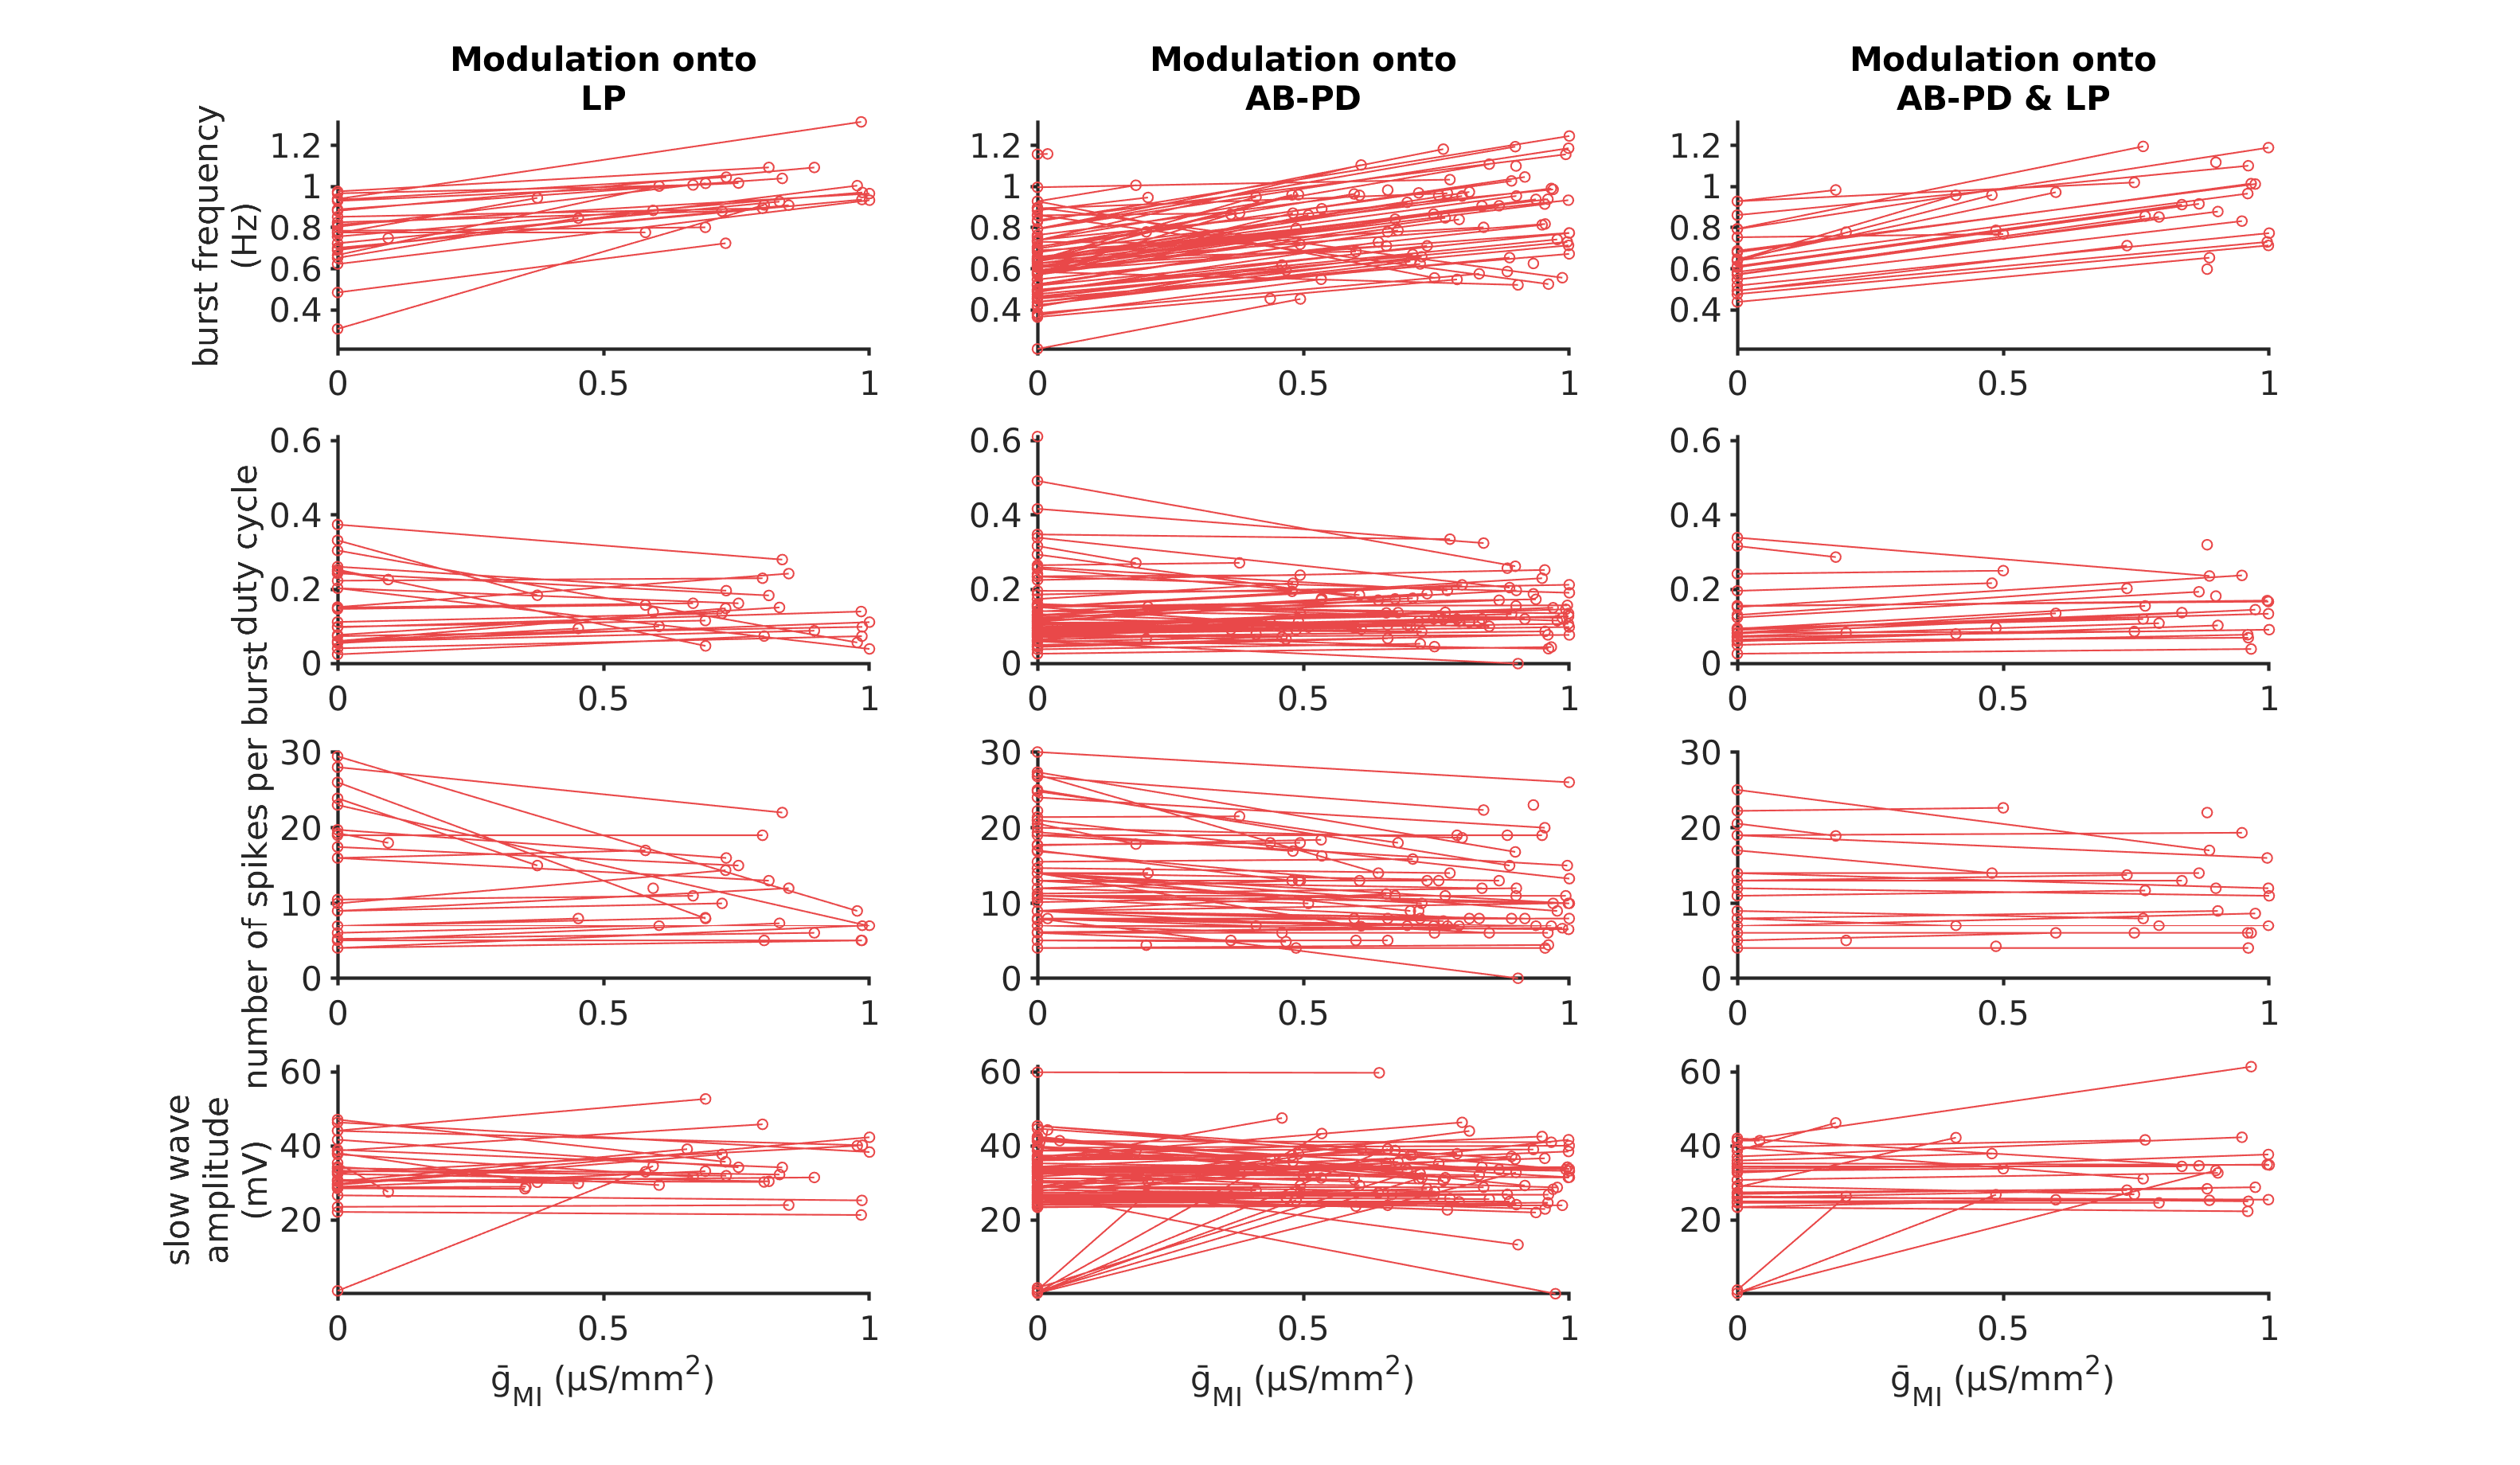
\includegraphics[width=1.0\linewidth]{gfx/all-modulation/metrics_LP}
	\caption[All optimized ABPD models in decentralized and modulated cases]{146 network models in decentralized and modulated cases show increased burst frequency and amplitude under modulated conditions with respect to decentralization. Modulation under \acs{AB}-\acs{PD} and \acs{LP} produces the most regular triphasic output. Colors indicate cells (red is \acs{LP}).}
	\label{fig:metricslp}
\end{figure}

\begin{figure}
	\centering
	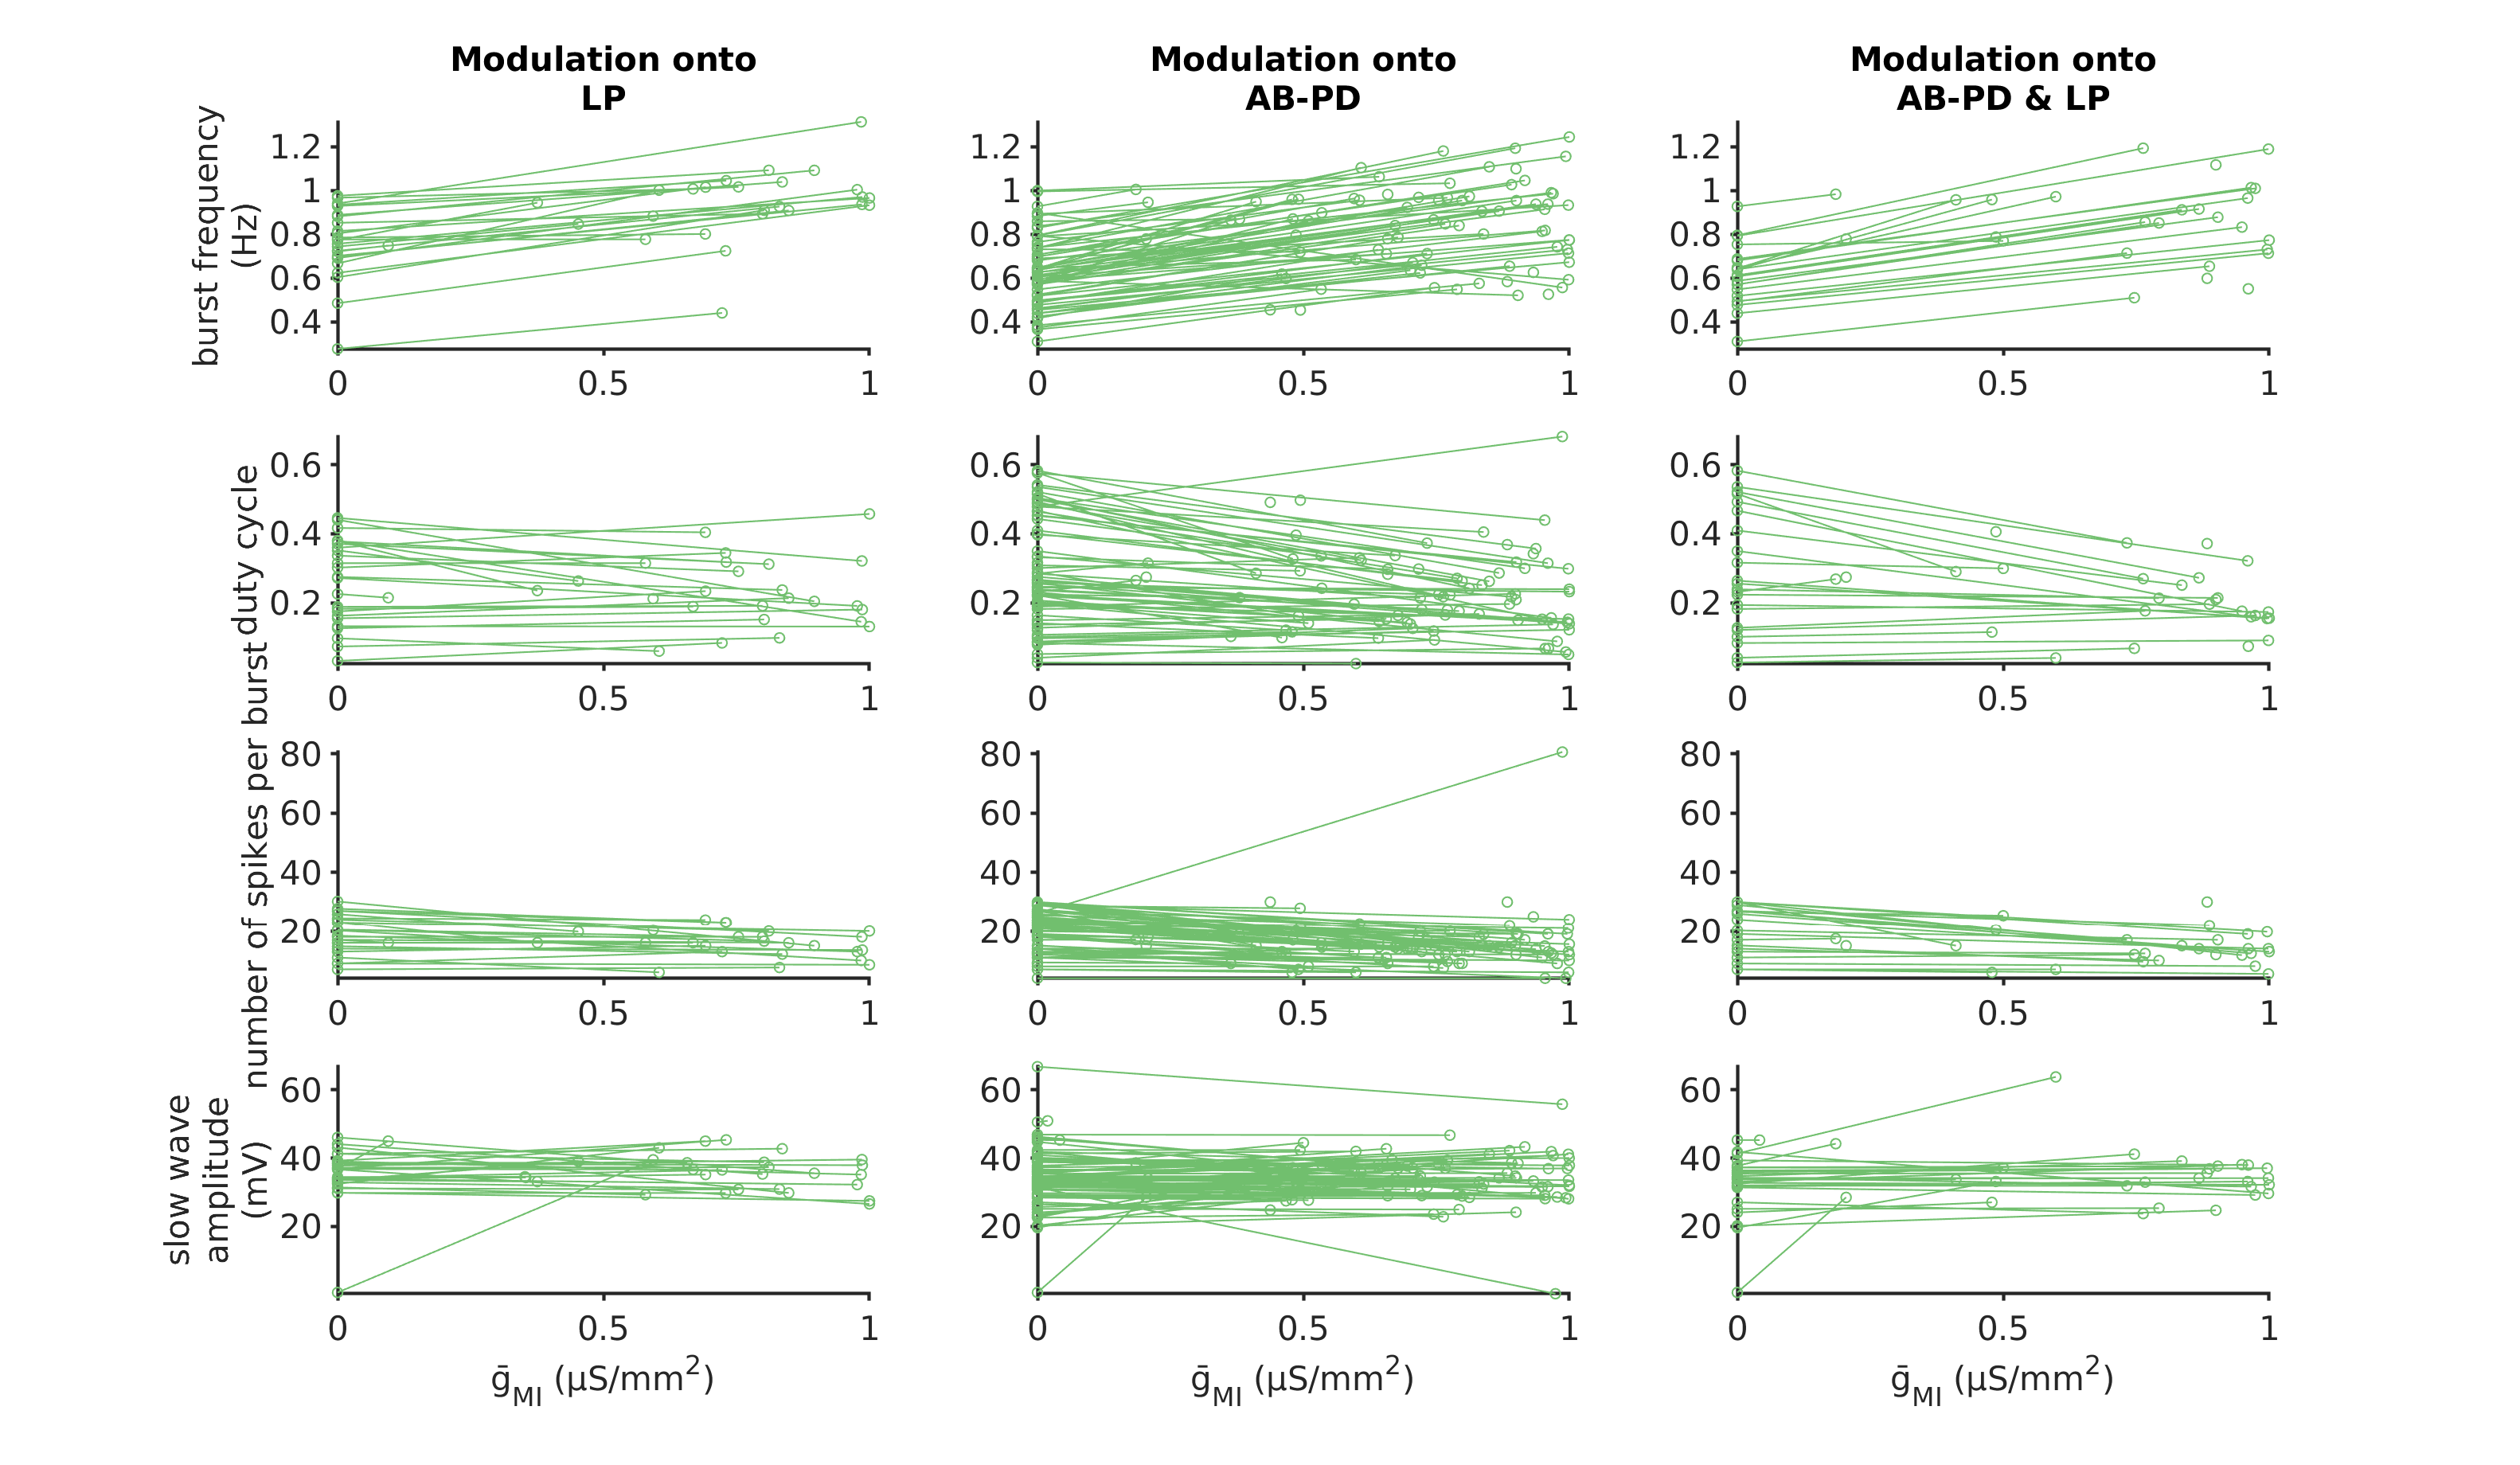
\includegraphics[width=1.0\linewidth]{gfx/all-modulation/metrics_PY}
	\caption[All optimized ABPD models in decentralized and modulated cases]{146 network models in decentralized and modulated cases show increased burst frequency and amplitude under modulated conditions with respect to decentralization. Modulation under \acs{AB}-\acs{PD} and \acs{LP} produces the most regular triphasic output. Colors indicate cells (green is \acs{PY}).}
	\label{fig:metricspy}
\end{figure}

\FloatBarrier

\subsection{Modulation of LP Can Inhibit AB-PD}

\autoref{fig:traces1} demonstrates a case where modulation onto \acs{LP} decreases \acs{AB}-\acs{PD} burst frequency, but modulation onto the pacemaker or \acs{AB}-\acs{PD} and \acs{LP} increases burst frequency. In \autoref{fig:metrics1}, the slow-wave amplitude and frequency of \acs{LP} increases, inhibiting the pacemaker, which bursts at a much slower frequency. If modulation is applied to \acs{AB}-\acs{PD} or the pacemaker kernel and \acs{LP}, the frequency increases. If the strength of the synapse is strong, pacemaker burst frequency decreases.

Applied current or \acs{IMI} tends to drive the rhythm, increasing burst frequency\autocite{DrionIonchanneldegeneracy2015,EisenMechanismsunderlyingpattern1982}. Modulation onto \acs{LP} inhibits the pacemaker, causing \acs{AB}-\acs{PD} to skip every other burst (\autoref{fig:traces2}). In both \autoref{fig:traces1} and \autoref{fig:traces2}, rhythmicity is maintained because synaptic transmission in the \acs{STG} is partially graded. Instead, if modulation is applied to the pacemaker kernel or the pacemaker kernel and \acs{LP}, the frequency increases by 60\% (\autoref{fig:traces2}). These models recapitulate the role of \acs{AB}-\acs{PD} as the pacemaker kernel in the pyloric circuit. 

Modulated neurons tend to maintain the same number of spikes per burst and duty cycle despite the higher frequency\autocite{EisenMechanismsunderlyingpattern1982,SwensenMultiplepeptidesconverge2000}. Those which are not modulated typically fall behind. This is likely due to the fact that modulation acts at the spike threshold but does not contribute significantly to the spiking waveform. Non-modulated cells experience increased inhibition in the same period of time; the membrane potential does not depolarize as much between bouts of inhibition, decreasing slow-wave amplitude.

\subsection{Modulation of AB Can Elicit Tonic Spiking}

In some cases in the model, modulation onto the pacemaker has deleterious effects on the rhythm. If \acs{AB}-\acs{PD} is depolarized by addition of inward current near the spiking threshold, rhythmicity is lost (\autoref{fig:traces3}); the neuron is close to a transition to a tonic spiking regime. If instead, \acs{LP} is modulated, increasing inhibition onto the pacemaker drives the frequency (\autoref{fig:metrics3}). Interestingly, in the case where \acs{IMI} activates in the pacemaker kernel and \acs{LP}, rhythmicity is maintained, and burst frequency and slow-wave amplitude increase.

This result is likely non-physiological. Injected current into \acs{AB} depolarizes the membrane, but generally does not elicit tonic spiking (\autoref{fig:sharp2})\autocite{SwensenModulatorsconvergentcellular2001,Soto-TrevinoComputationalmodelelectrically2005}. The pacemaker is also not readily susceptible loss of rhythmicity from hyperpolarization due to a constant current\autocite{Soto-TrevinoComputationalmodelelectrically2005}. The modulatory input recorded in \citeauthor{SwensenModulatorsconvergentcellular2001}\autocite{SwensenModulatorsconvergentcellular2001} cannot produce the sustained excitatory or inhibitory pulses of current necessary to cease endogenous bursting. In light of this, modulation onto \acs{LP} contributes less to the increase in burst frequency and amplitude seen with proctolin and \acs{RPCH}. 

Given that most \acs{AB}-\acs{PD} pacemakers must be far from transitions into depolarization block and tonic spiking regimes and be robust to hyperpolarization\autocite{WeimannModulationOscillatorInteractions1997,Harris-WarrickDynamicBiologicalNetworks1992}, the models suggest that modulation of \acs{LP} likely serves an ancillary role in in initiation and maintenance of robust triphasic motor patterns. These conclusions are supported by experiments with \ac{CCAP}, in which modulation of \acs{LP} while the pacemaker was hyperpolarized was insufficient to initiate the pyloric rhythm\autocite{WeimannModulationOscillatorInteractions1997}.

\FloatBarrier

\begin{figure}[t]
	\centering
	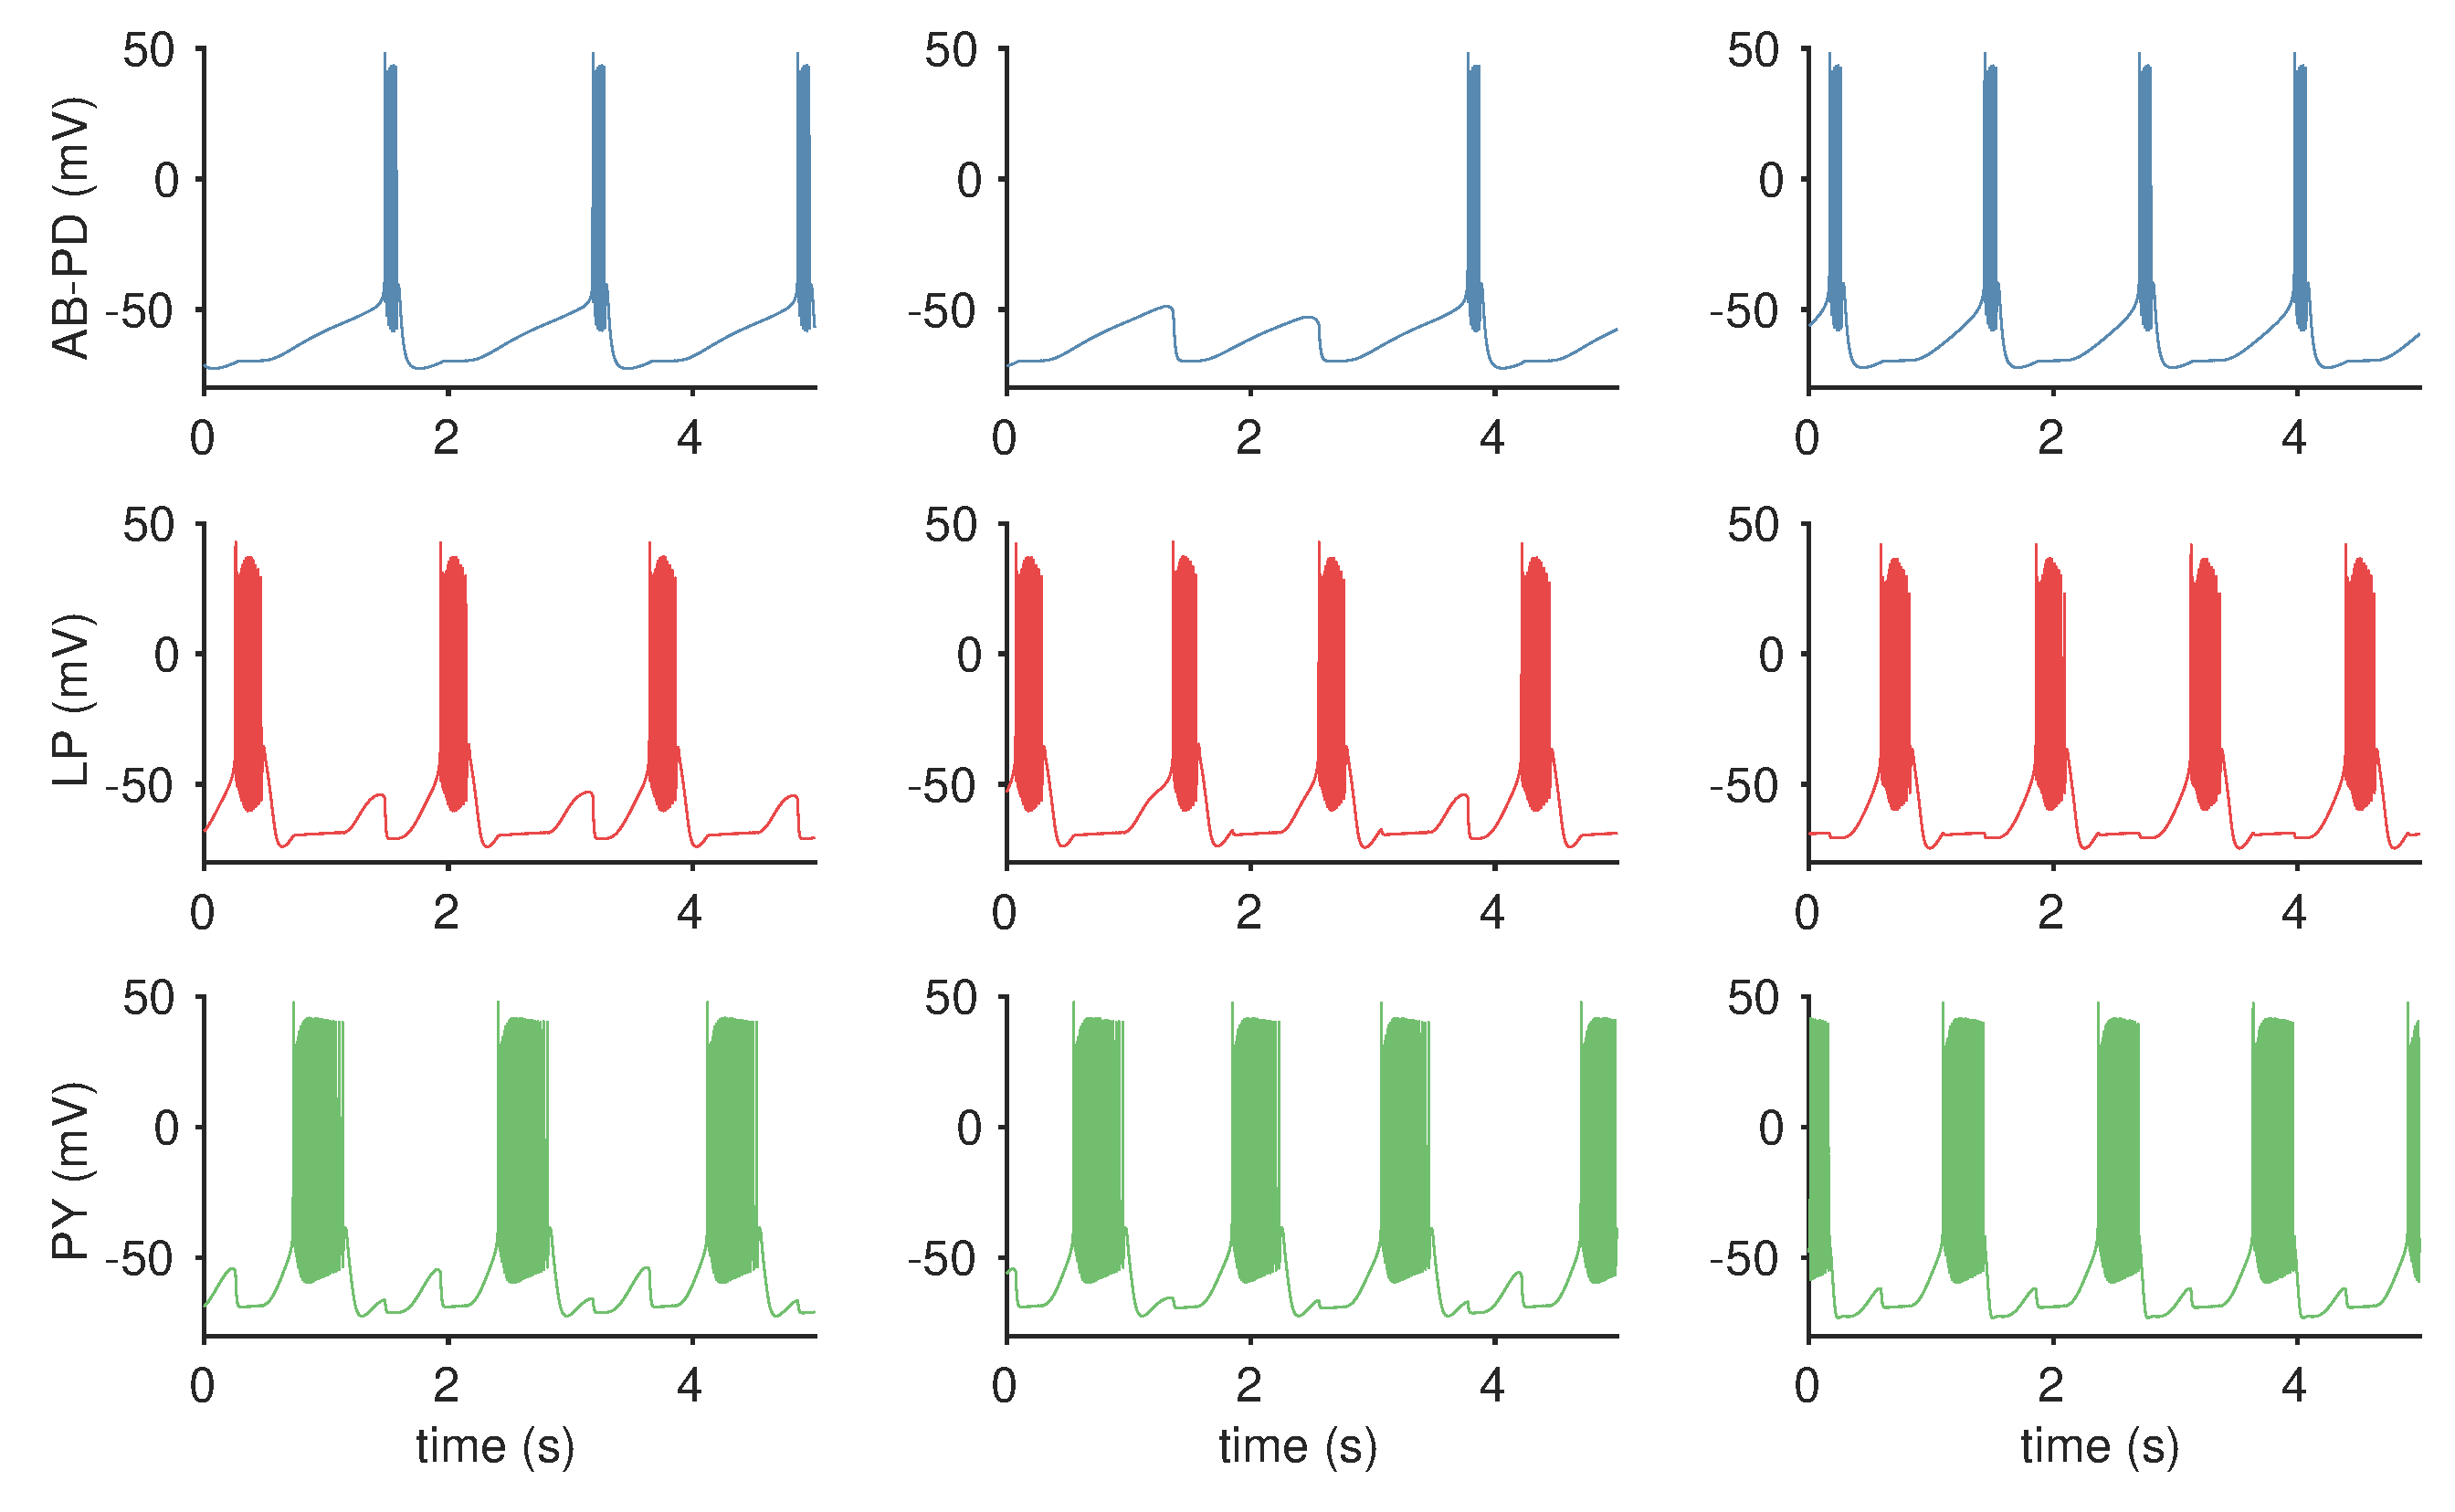
\includegraphics[width=1.0\linewidth]{gfx/all-modulation/traces1}
	\caption[Modulation onto LP inhibits the pacemaker (traces)]{Neuromodulation onto \acs{LP} can inhibit the pacemaker. Cells in columns are in the same network. \textit{Left:} No neuromodulation and a normal triphasic rhythm. \textit{Middle:} $\bar{g}_{MI}^{LP} = 0.2~\mu \mathrm{S/mm^2}$, the pacemaker is inhibited by \acs{LP}. \textit{Right:} Recovery, where $\bar{g}_{MI}^{LP} = \bar{g}_{MI}^{AB-PD} = 0.6~\mu \mathrm{S/mm^2}$, normal triphasic rhythm with increased frequency.}
	\label{fig:traces1}
\end{figure}

\begin{figure}[b]
	\centering
	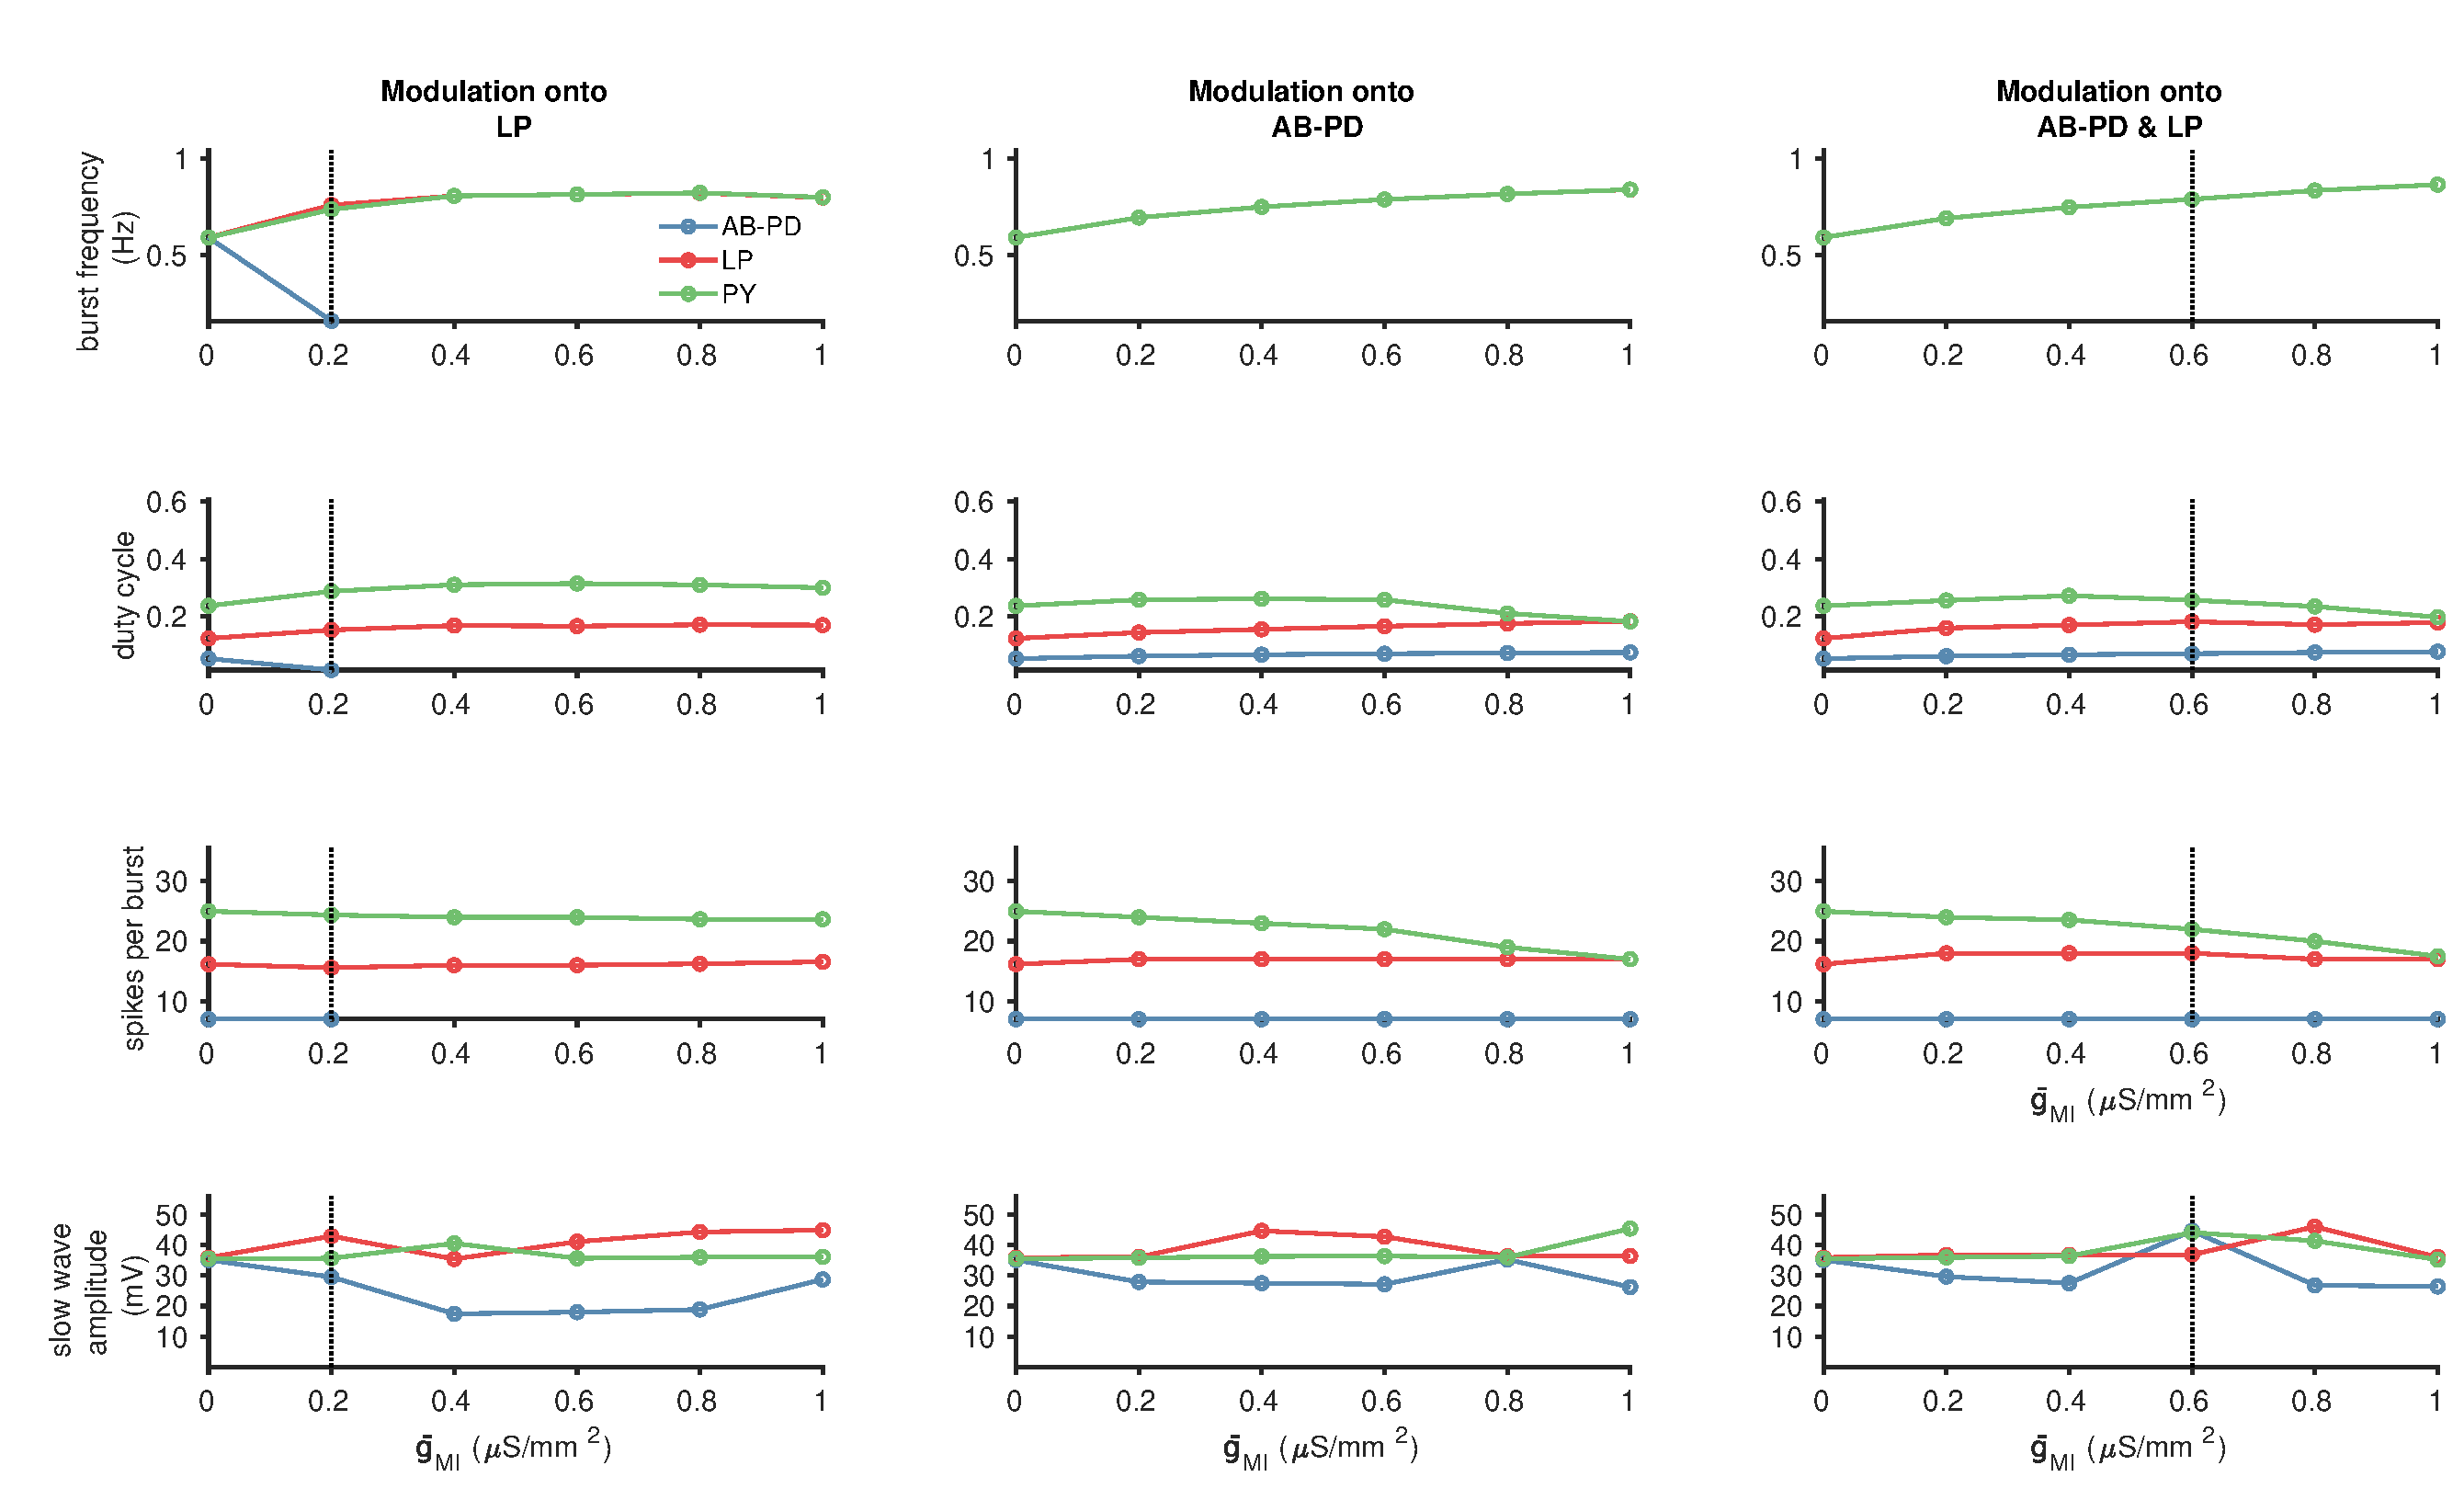
\includegraphics[width=1.0\linewidth]{gfx/all-modulation/metrics1}
	\caption[Modulation onto LP inhibits the pacemaker (metrics)]{Neuromodulation onto \acs{LP} can inhibit the pacemaker. Columns display metrics calculated at steady-state for three cases of modulation. Colors indicate cells (blue is \acs{AB}-\acs{PD}, red is \acs{LP}, green is \acs{PY}). Voltage traces at the dotted lines are shown in \autoref{fig:traces1}.}
	\label{fig:metrics1}
\end{figure}

\FloatBarrier

\begin{figure}[t]
	\centering
	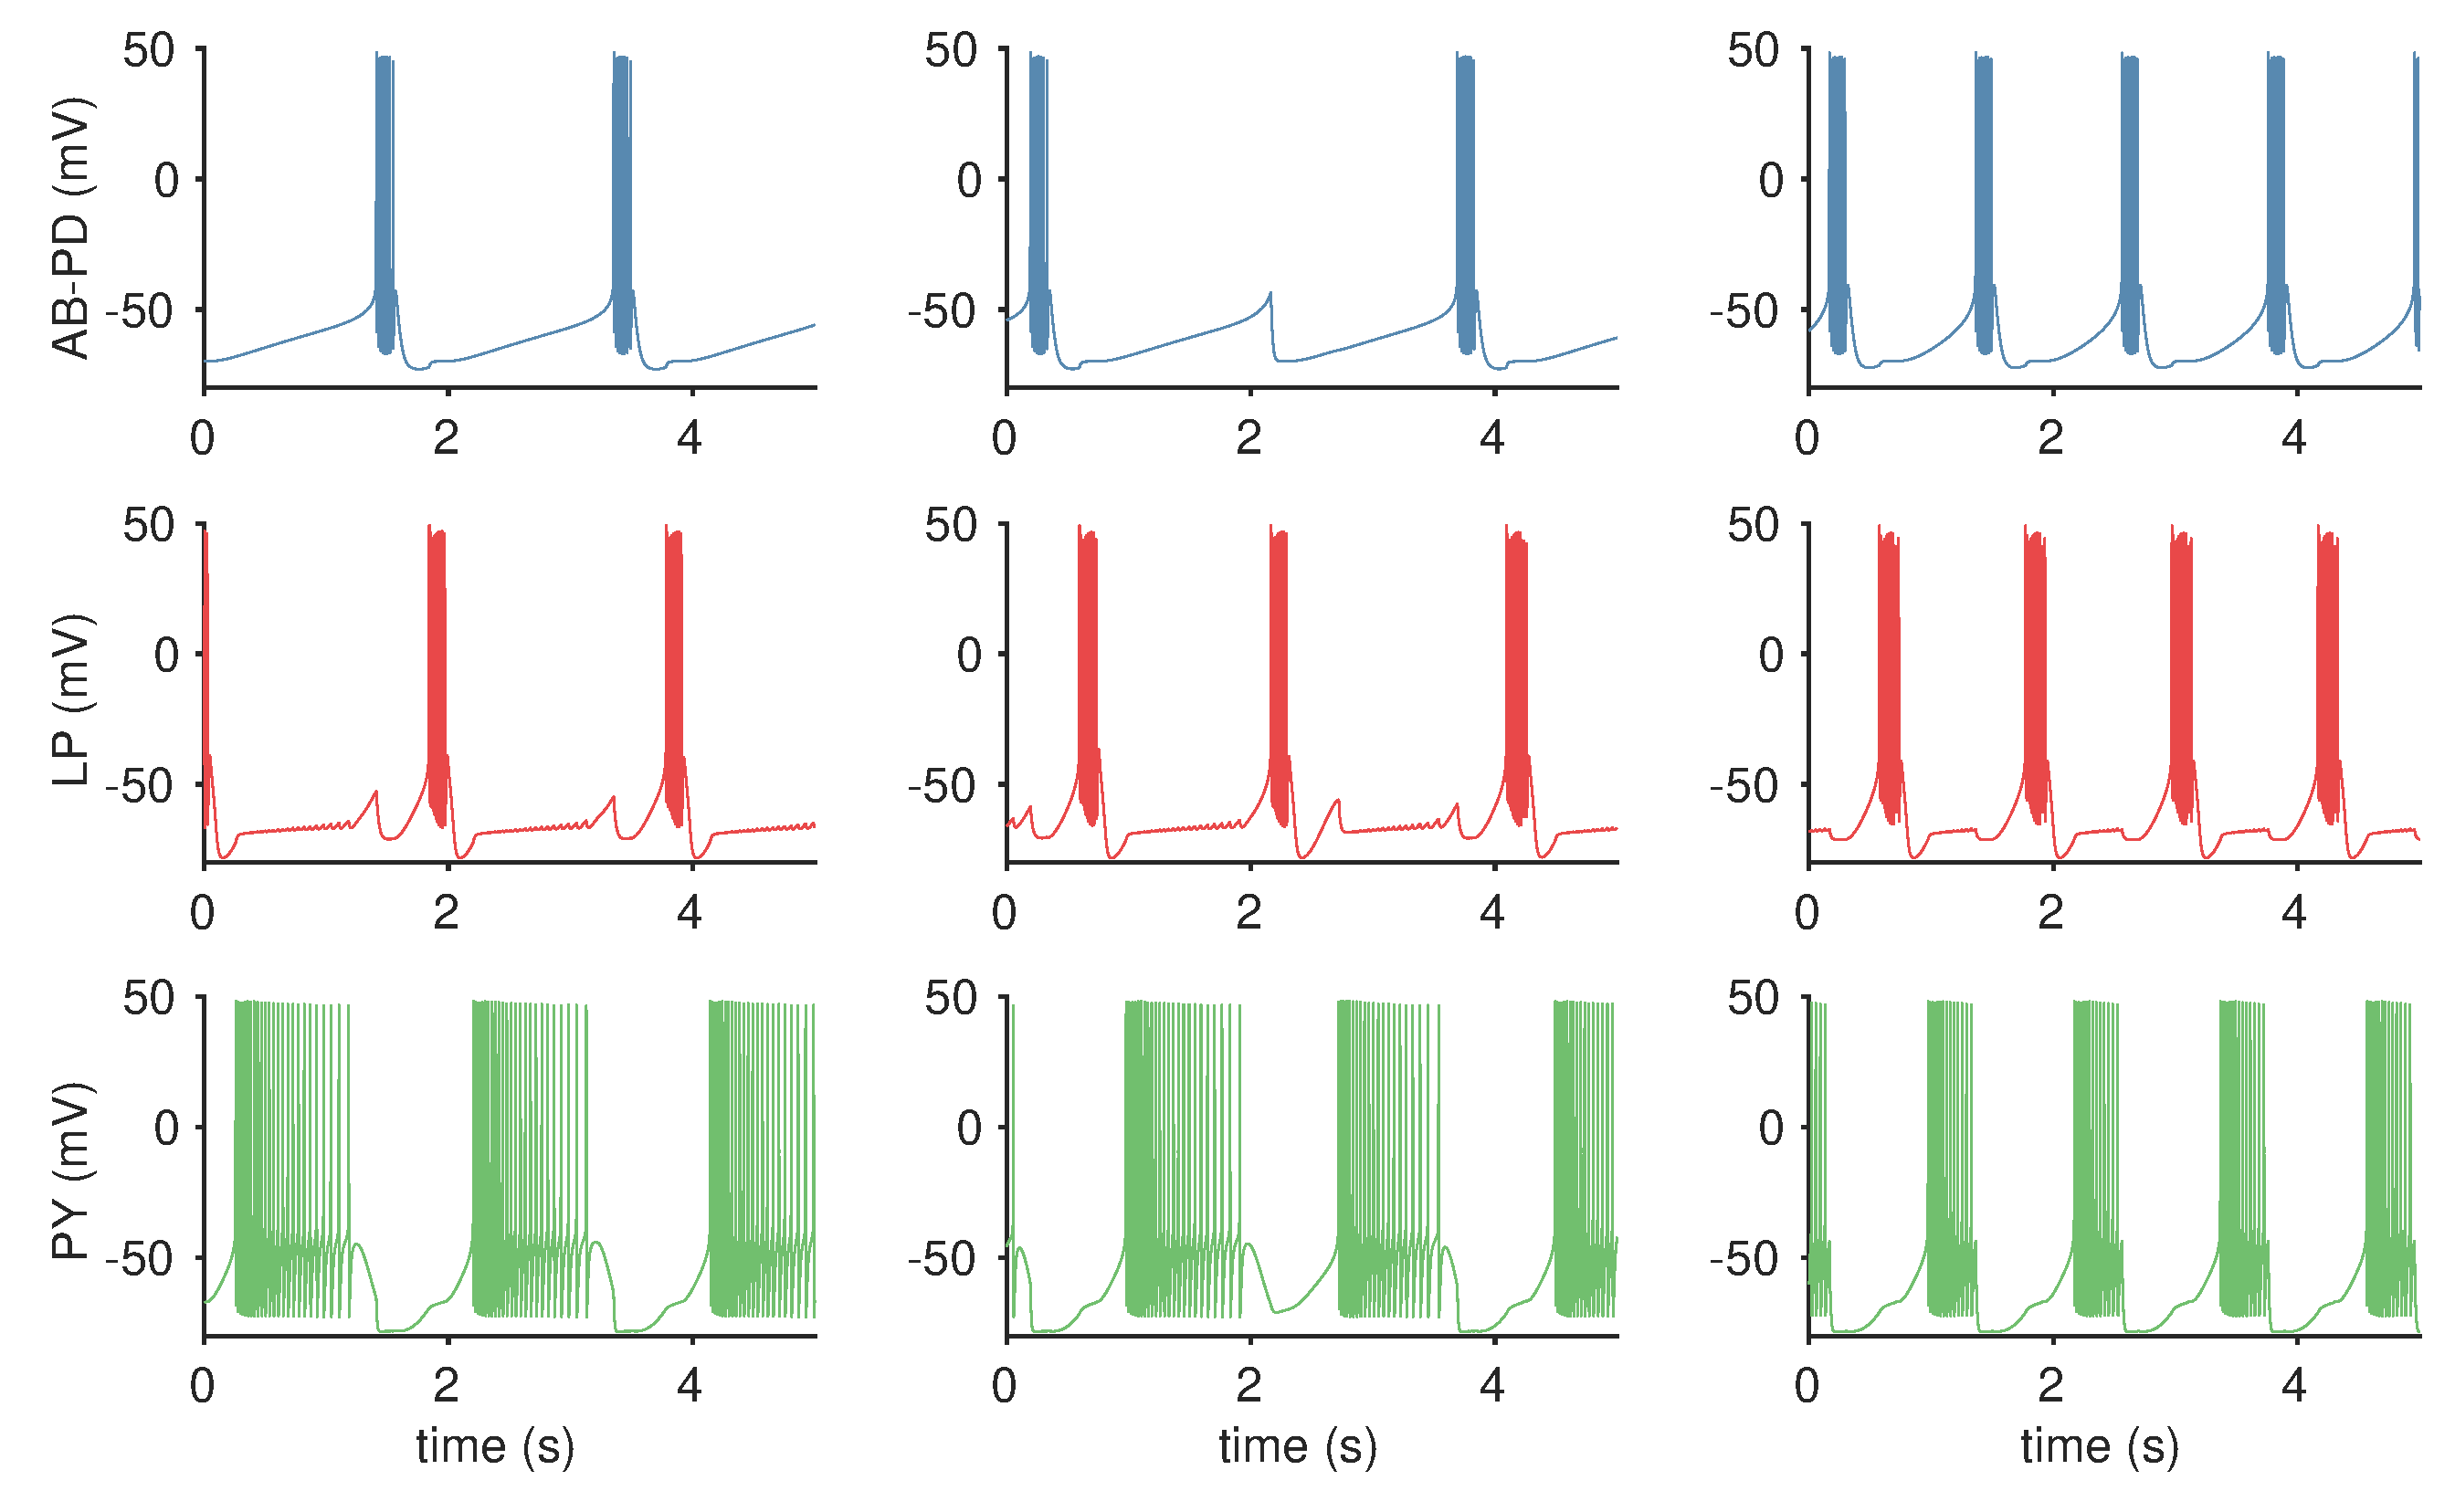
\includegraphics[width=1.0\linewidth]{gfx/all-modulation/traces2}
	\caption[Modulation onto LP does not increase frequency (traces)]{Neuromodulation onto \acs{LP} does not increase burst frequency. Cells in columns are in the same network. \textit{Left:} No neuromodulation and a normal triphasic rhythm. \textit{Middle:} $\bar{g}_{MI}^{LP} = 0.8~\mu \mathrm{S/mm^2}$, \acs{LP} inhibits \acs{AB}-\acs{PD}. \textit{Right:} Recovery, where $\bar{g}_{MI}^{LP} = \bar{g}_{MI}^{AB-PD} = 1.0~\mu \mathrm{S/mm^2}$, normal triphasic rhythm with increased frequency.}
	\label{fig:traces2}
\end{figure}

\begin{figure}[b]
	\centering
	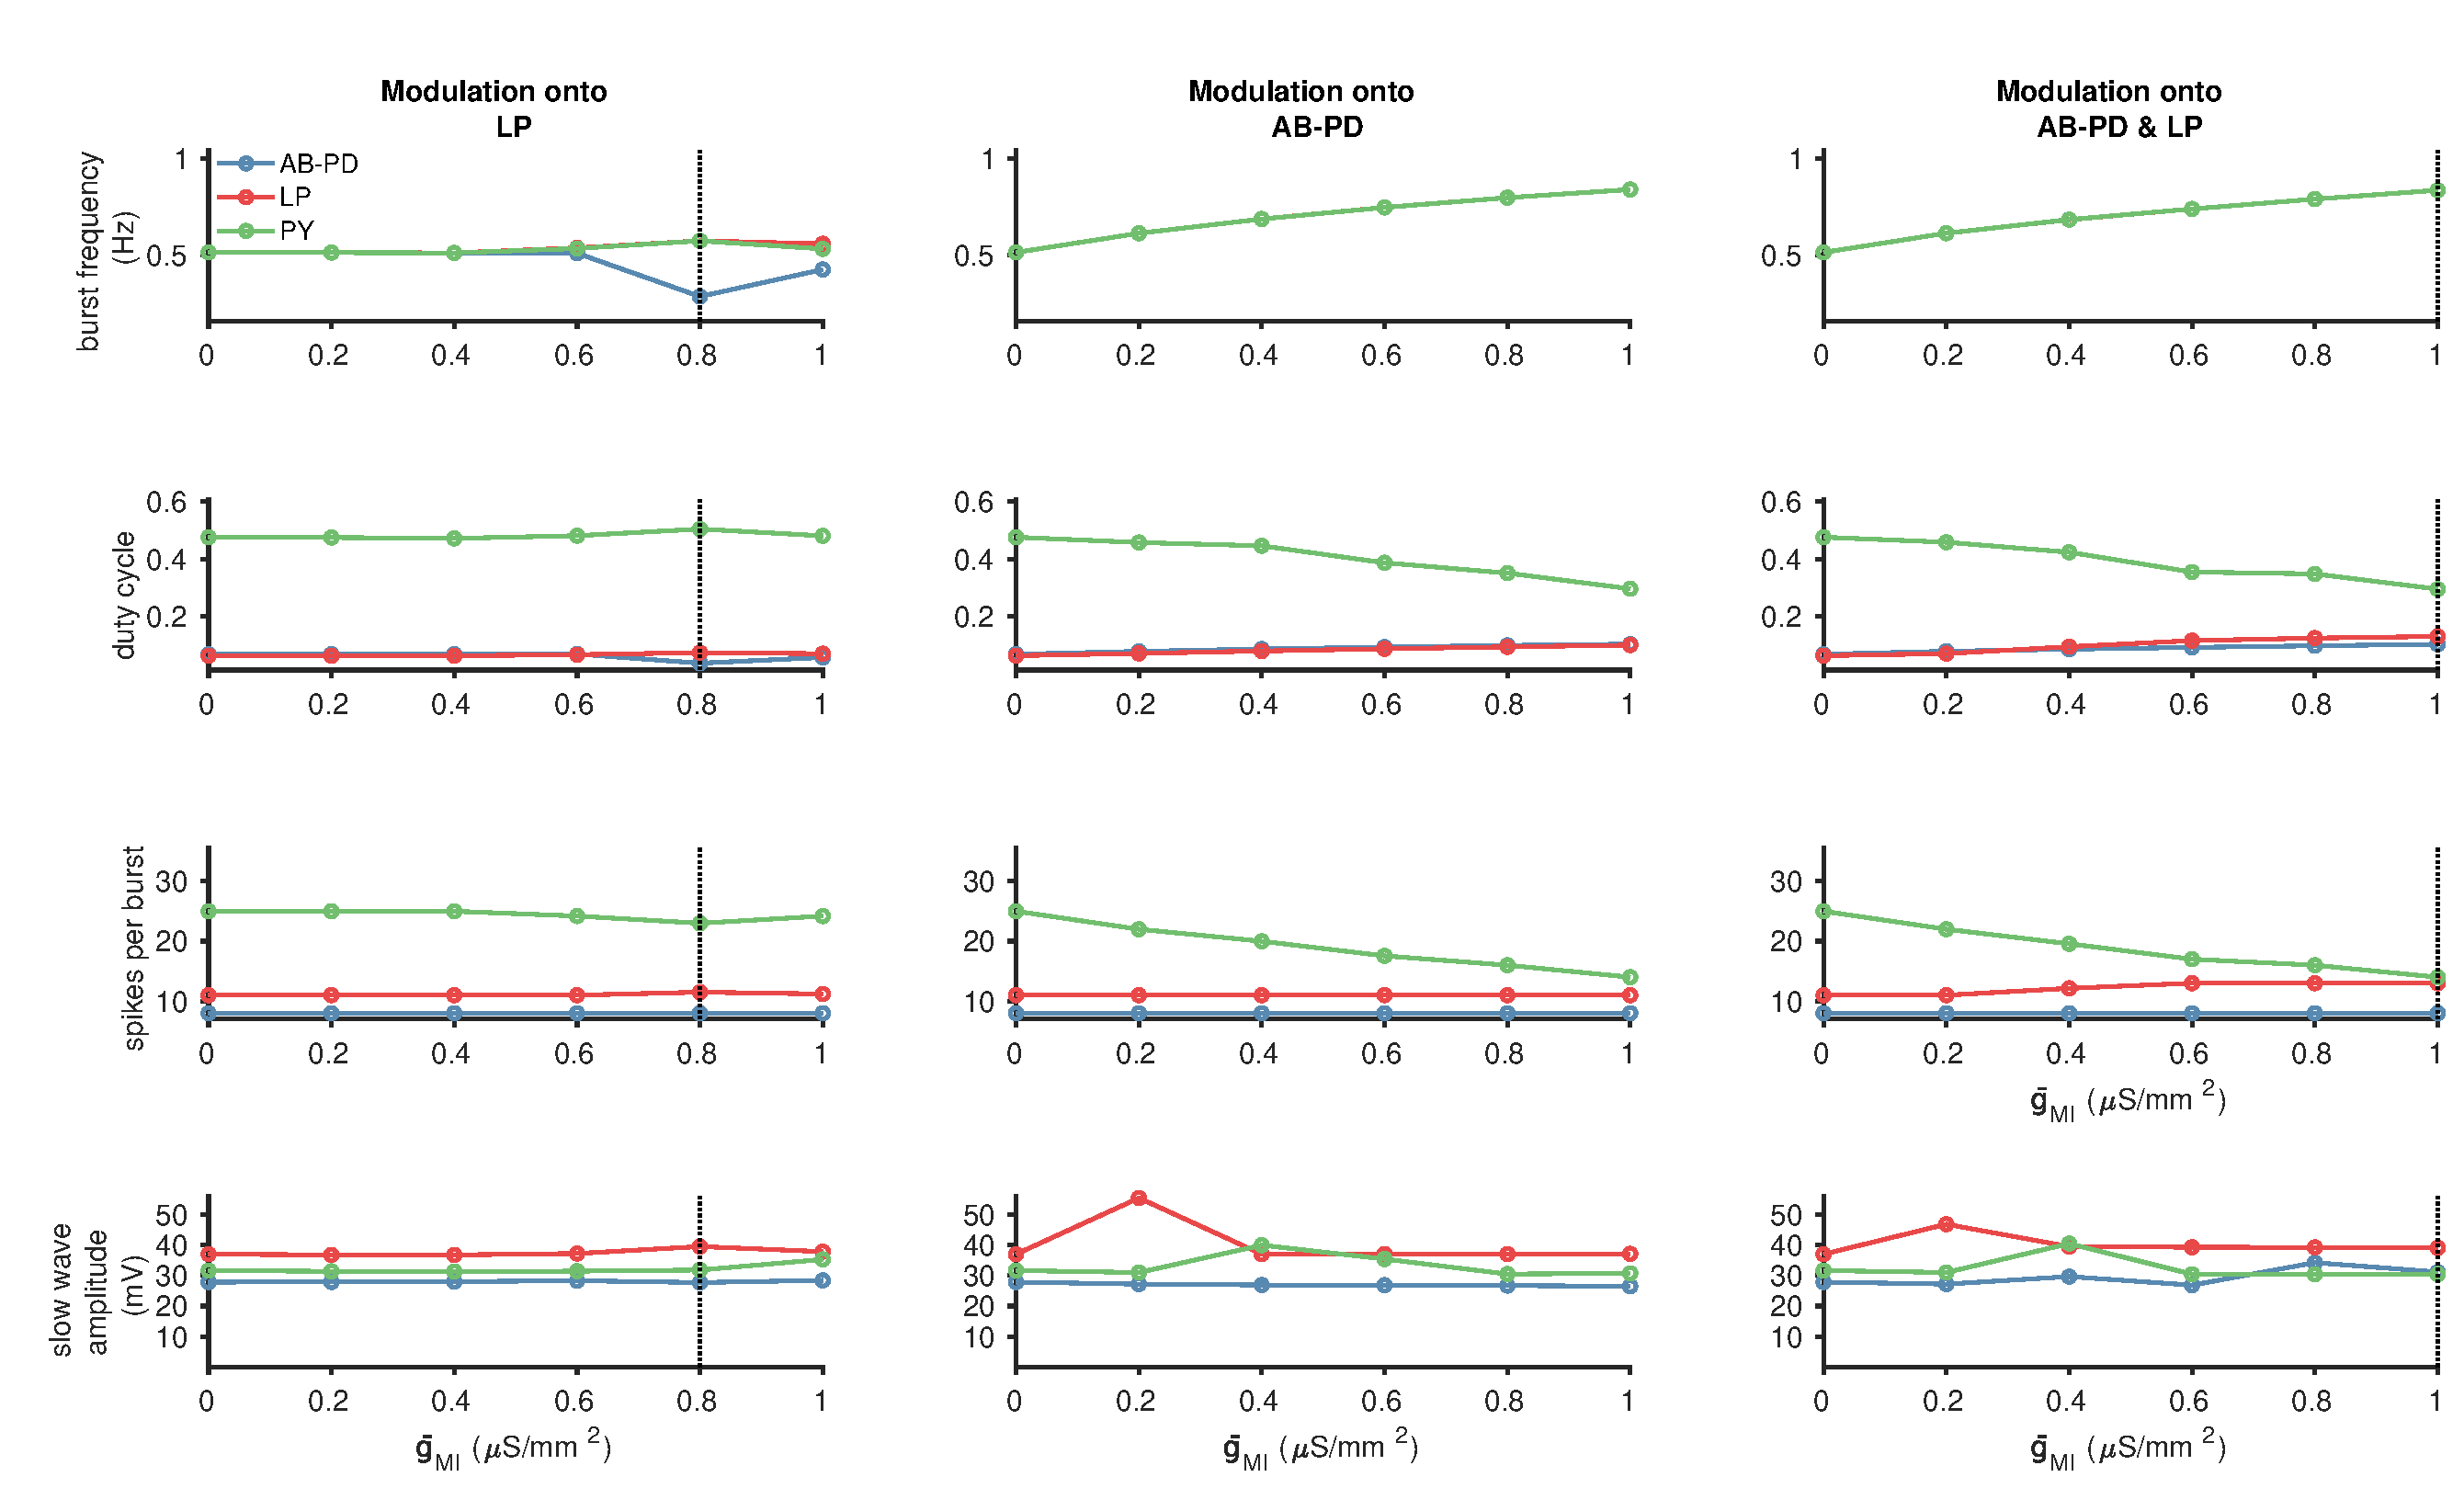
\includegraphics[width=1.0\linewidth]{gfx/all-modulation/metrics2}
	\caption[Modulation onto LP does not increase frequency (metrics)]{Neuromodulation onto \acs{LP} does not increase burst frequency in many models. Columns display metrics calculated at steady-state for three cases of modulation. Colors indicate cells (blue is \acs{AB}-\acs{PD}, red is \acs{LP}, green is \acs{PY}). Voltage traces at the dotted lines are shown in \autoref{fig:traces2}.}
	\label{fig:metrics2}
\end{figure}

\FloatBarrier

\begin{figure}[t]
	\centering
	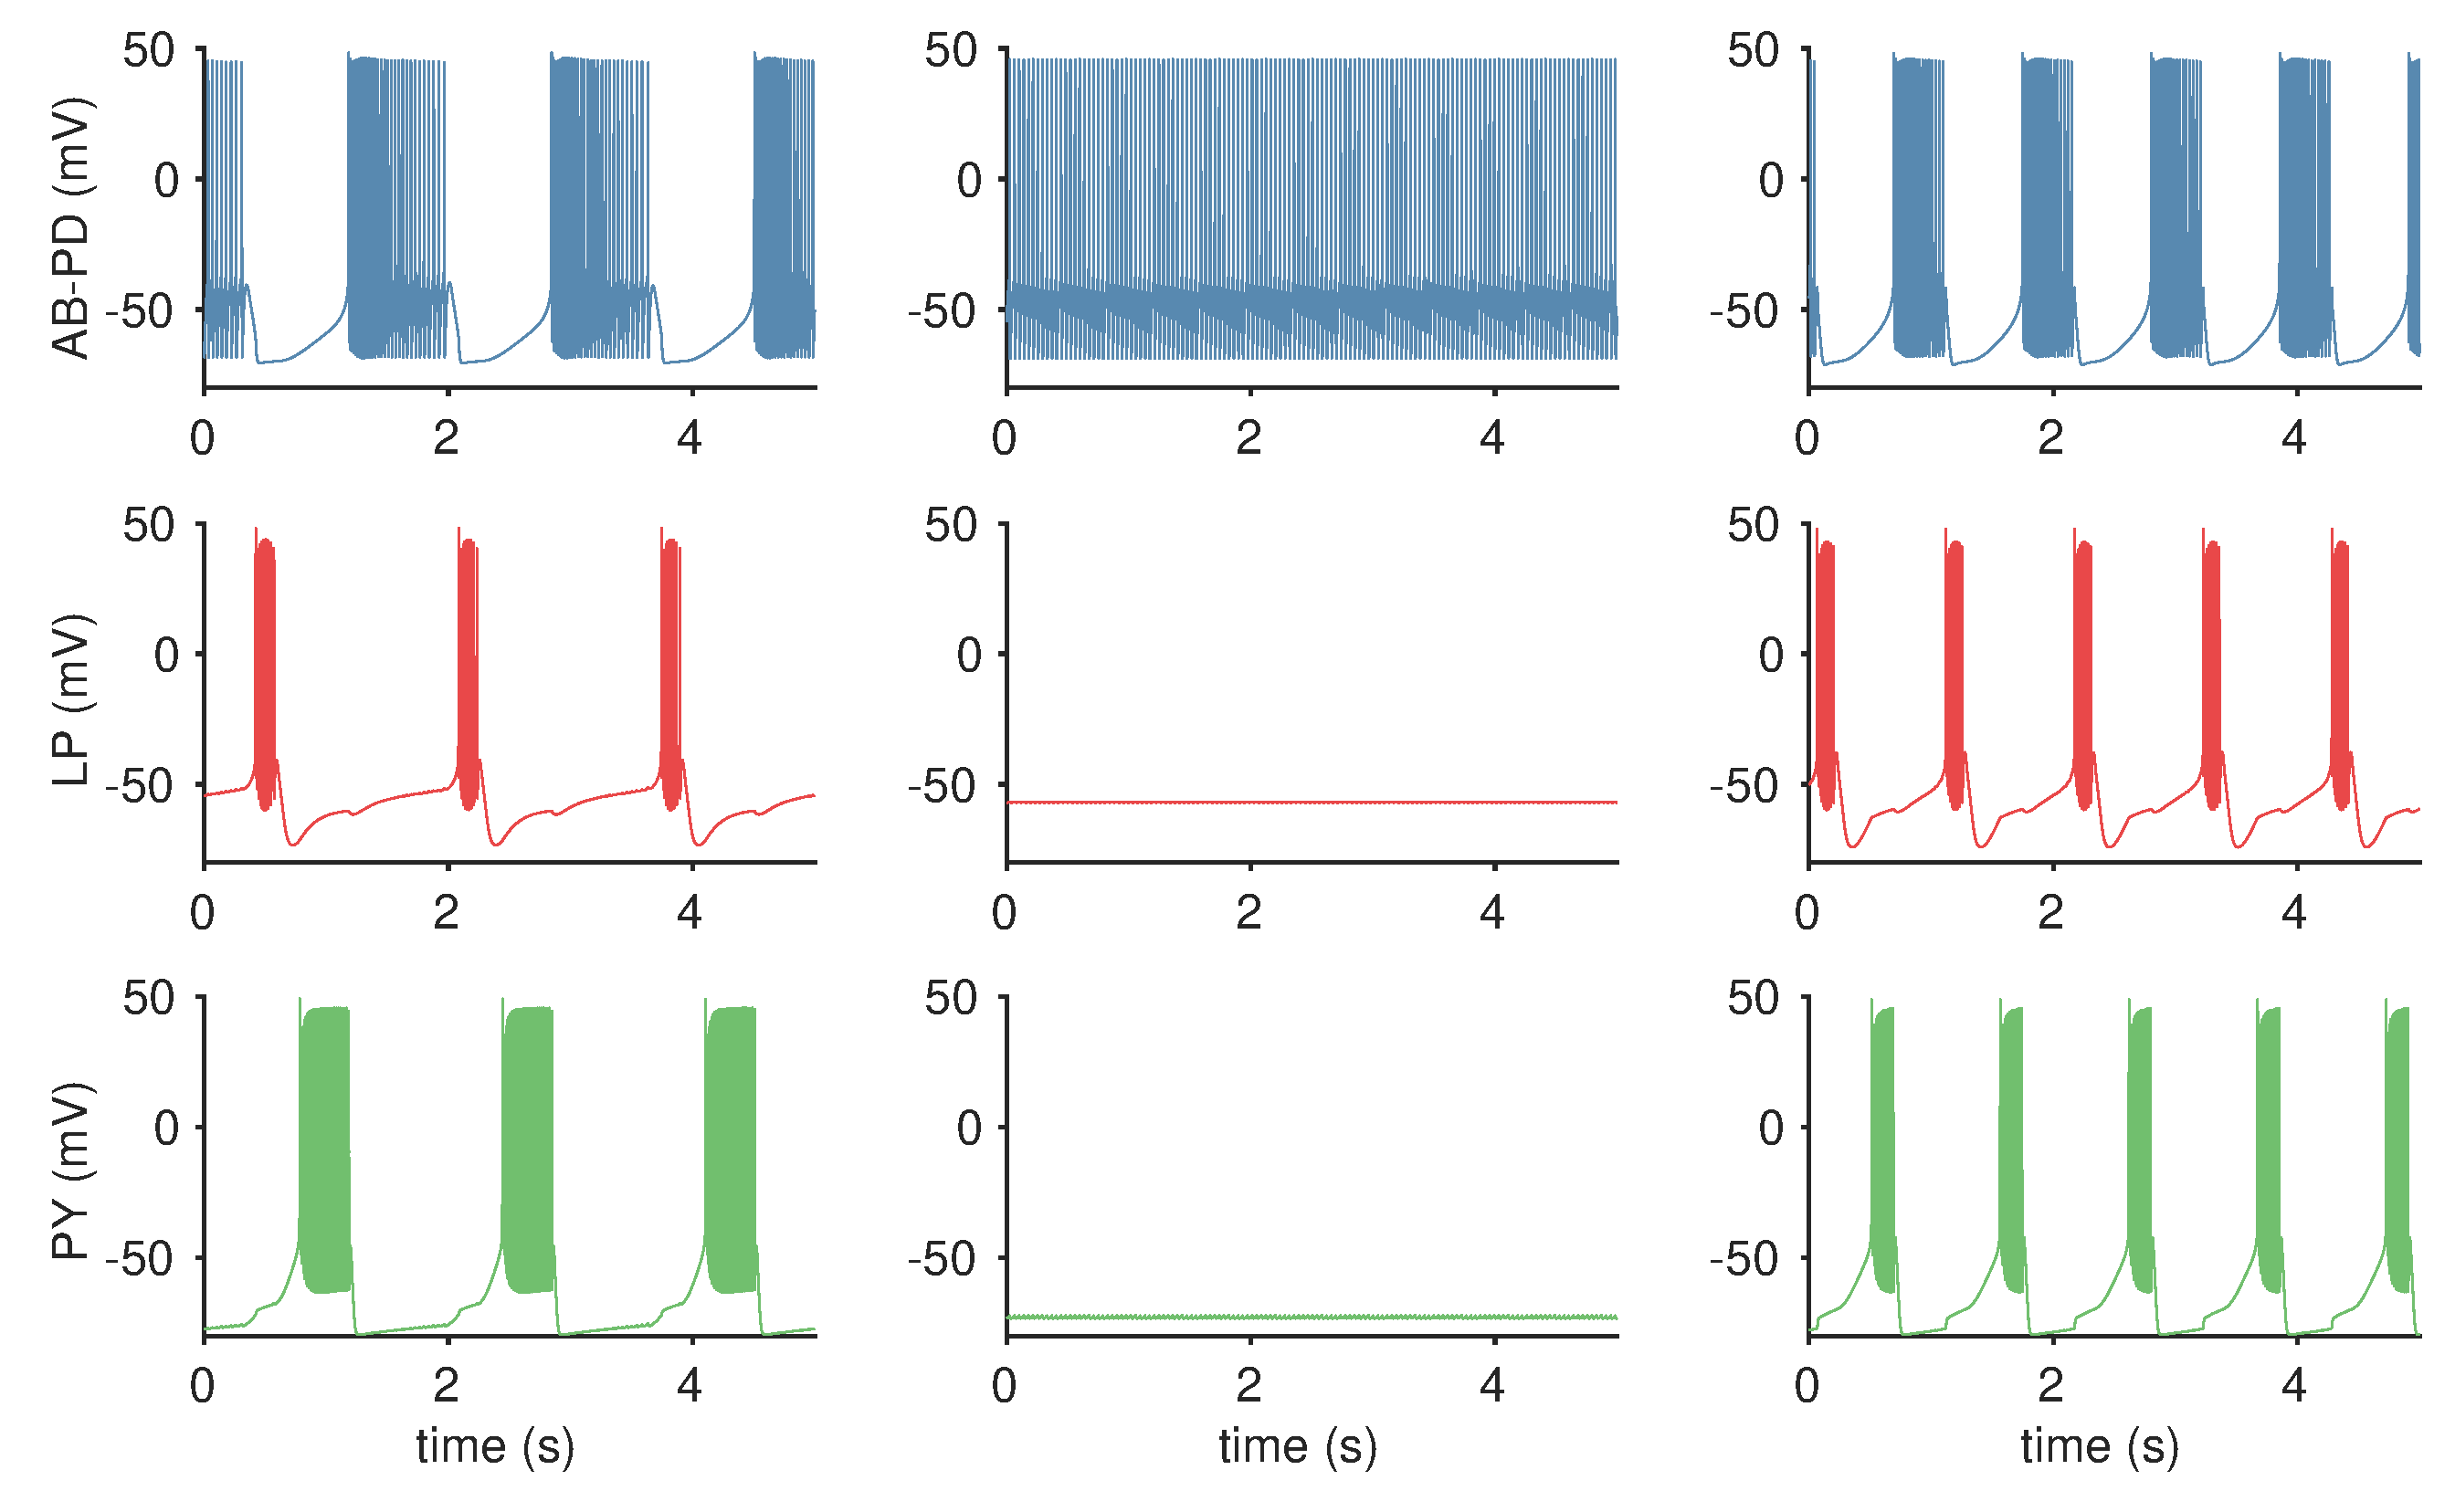
\includegraphics[width=1.0\linewidth]{gfx/all-modulation/traces3}
	\caption[Modulation of AB-PD depolarizes AB-PD (traces)]{Neuromodulation onto \acs{AB}-\acs{PD} can depolarize \acs{AB}-\acs{PD}. Cells in columns are in the same network. \textit{Left:} No neuromodulation and a normal triphasic rhythm. \textit{Middle:} $\bar{g}_{MI}^{AB-PD} = 0.6~\mu \mathrm{S/mm^2}$, \acs{AB}-\acs{PD} is tonically spiking. \textit{Right:} Normal triphasic rhythm, where $\bar{g}_{MI}^{LP} = \bar{g}_{MI}^{AB-PD} = 1.0~\mu \mathrm{S/mm^2}$, normal triphasic rhythm with increased frequency.}
	\label{fig:traces3}
\end{figure}

\begin{figure}[b]
	\centering
	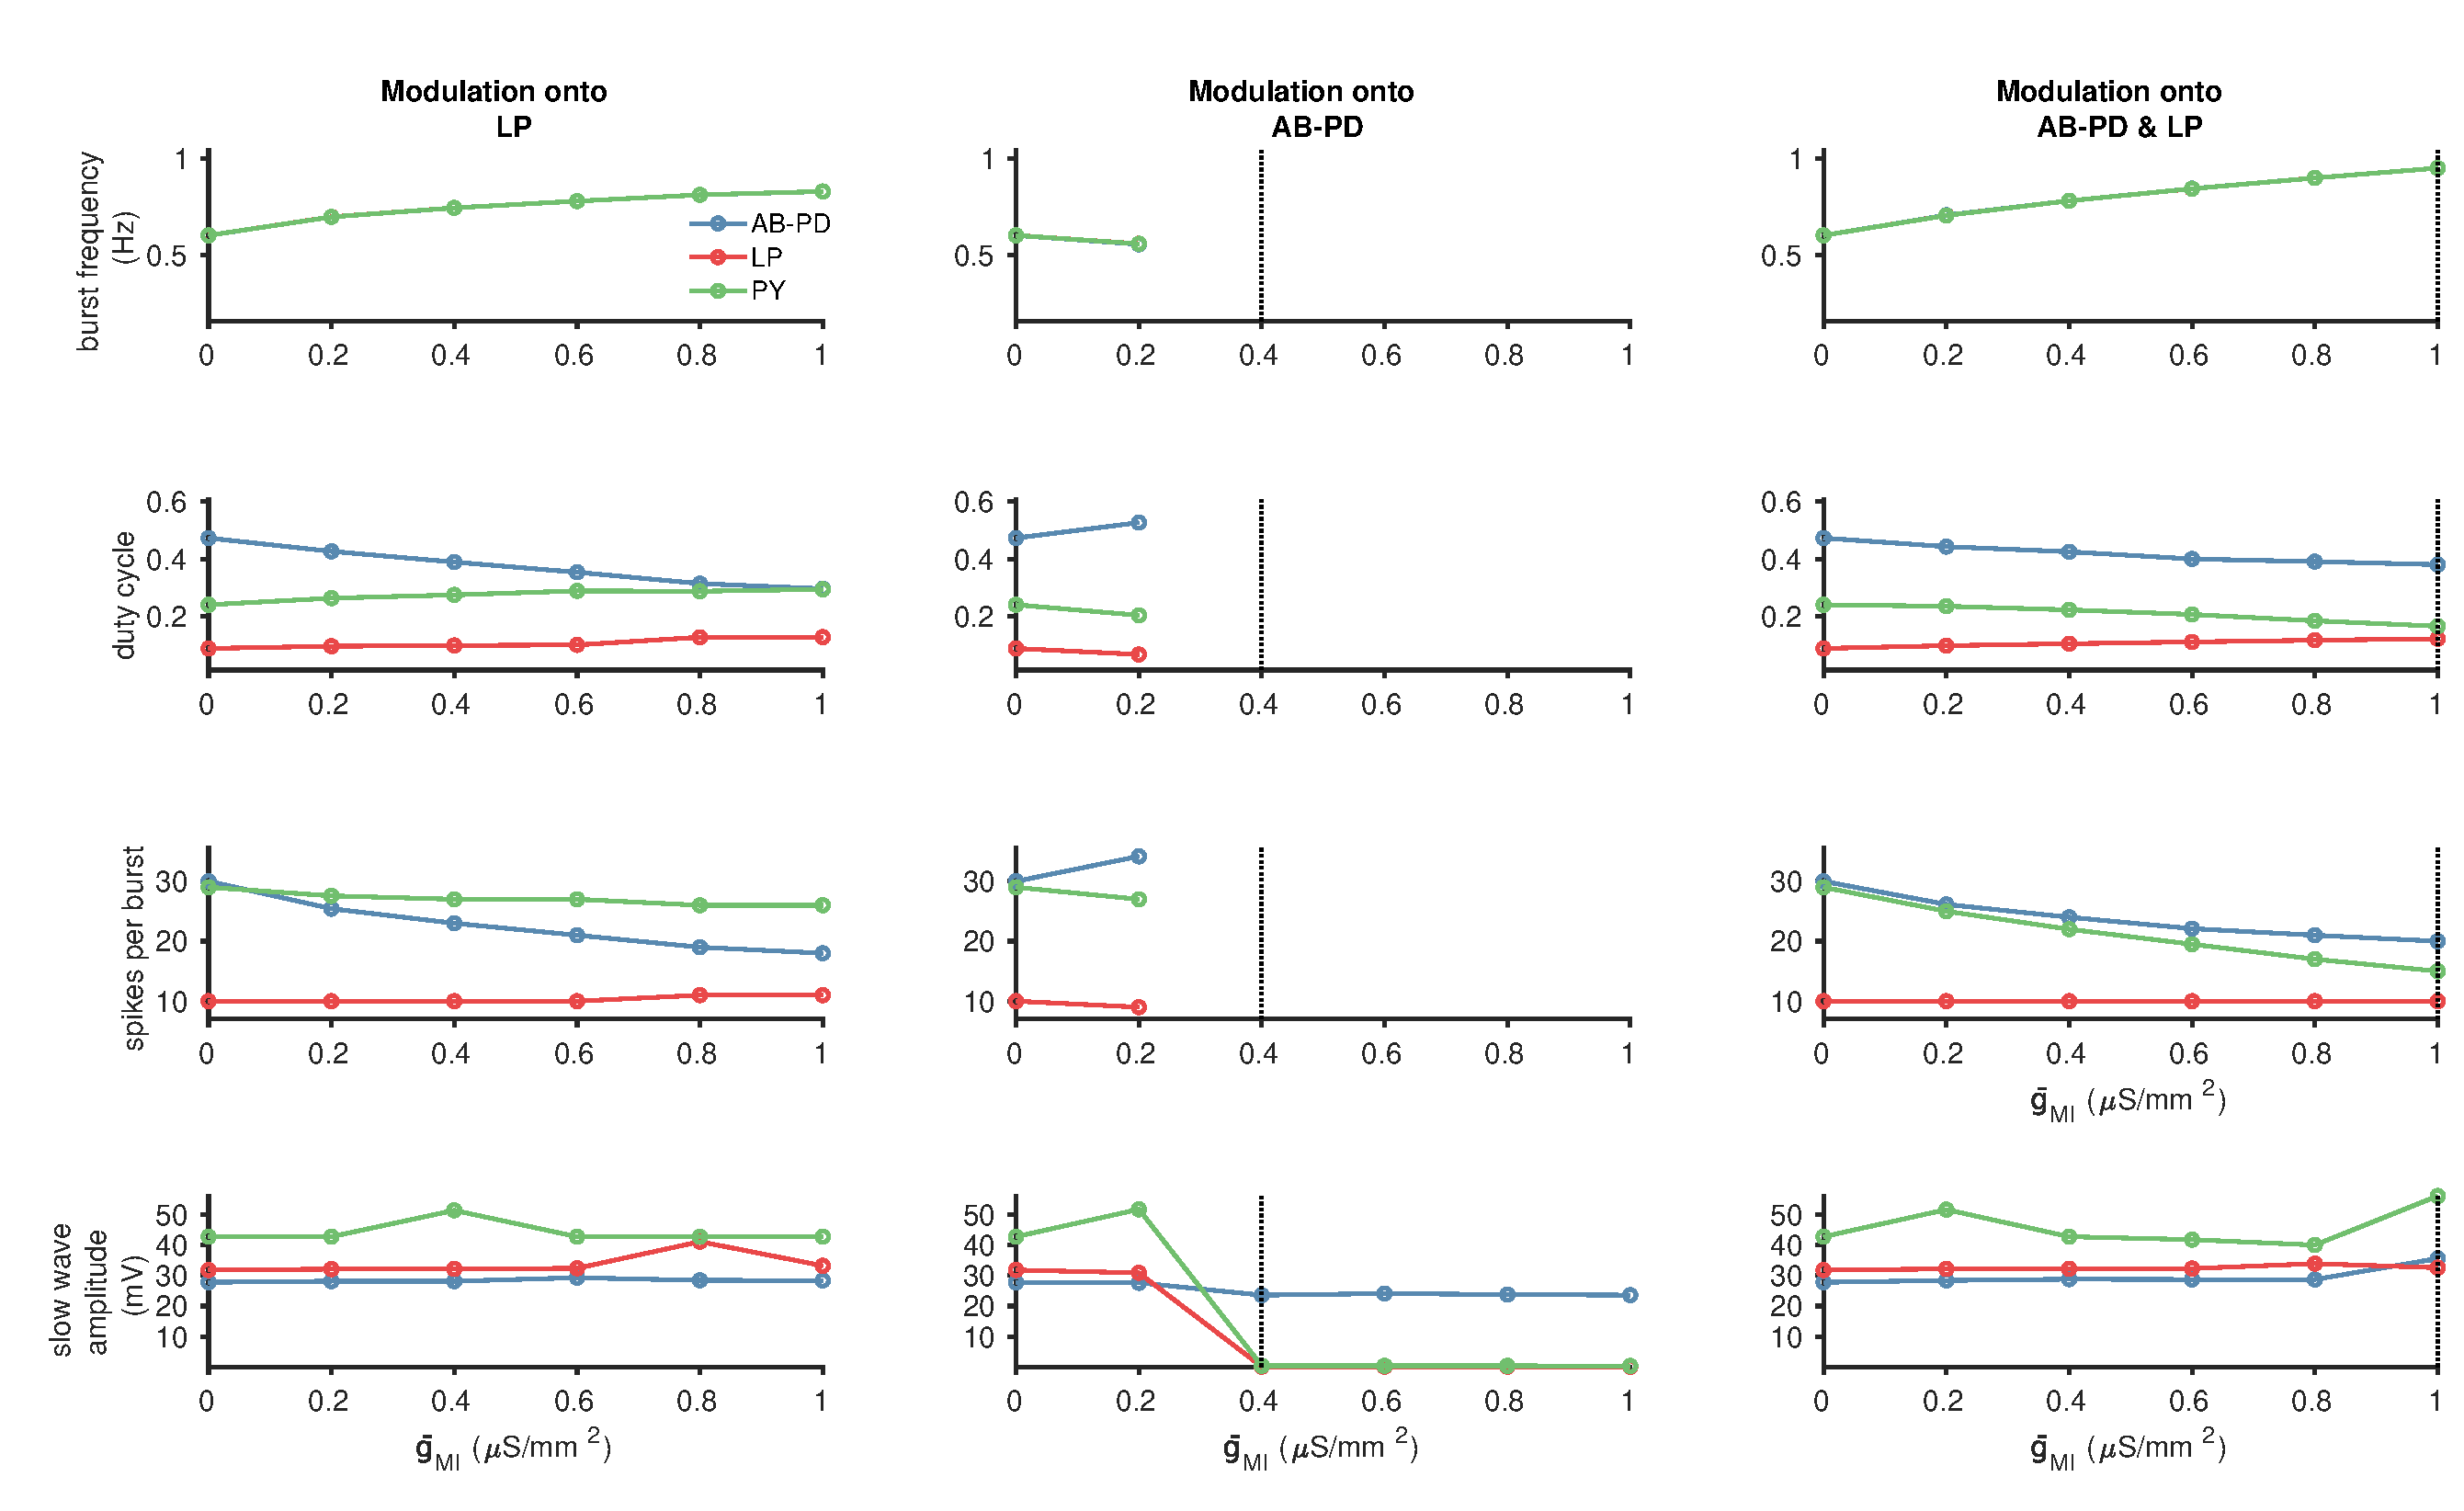
\includegraphics[width=1.0\linewidth]{gfx/all-modulation/metrics3}
	\caption[Modulation of AB-PD depolarizes AB-PD (metrics)]{Modulation onto \acs{AB}-\acs{PD} can depolarize the pacemaker, resulting in tonic spiking. Modulation of \acs{LP} or \acs{AB}-\acs{PD} and \acs{LP} results in normal triphasic rhythm with increasing burst frequency. Voltage traces at the dotted lines are shown in \autoref{fig:traces3}.}
	\label{fig:metrics3}
\end{figure}

\FloatBarrier

\begin{figure}[t]
	\centering
	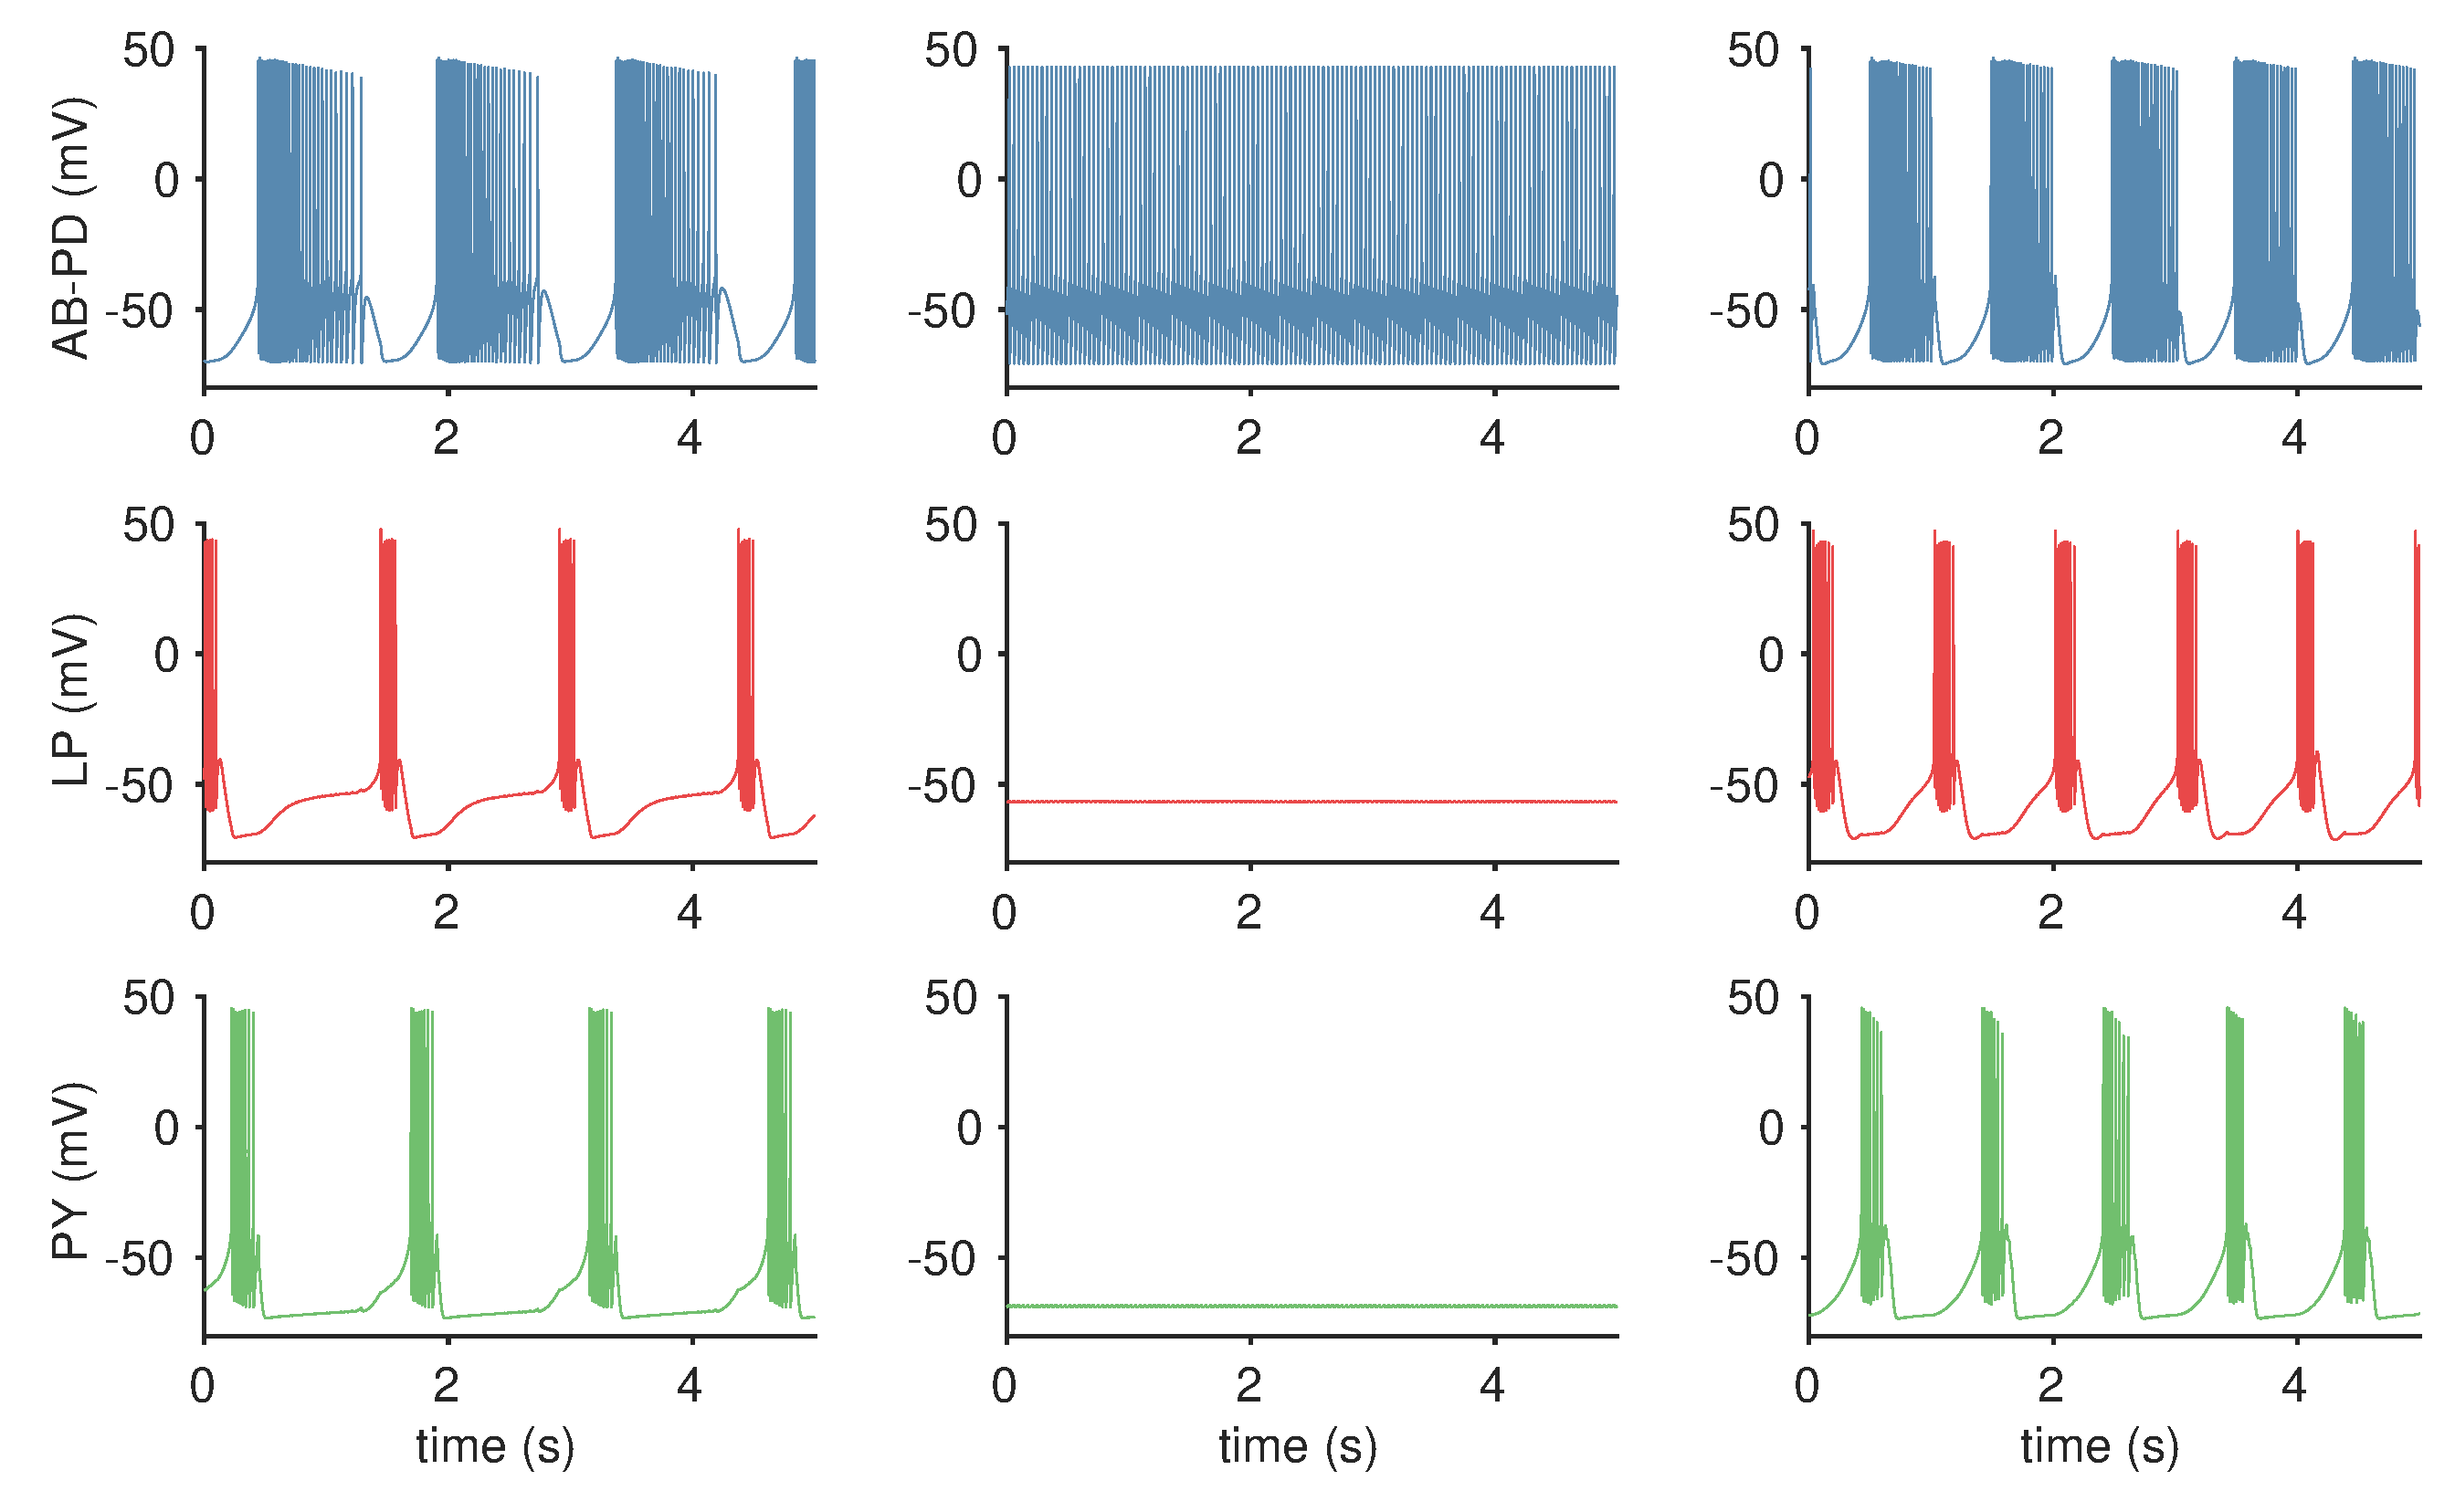
\includegraphics[width=1.0\linewidth]{gfx/all-modulation/traces4}
	\caption[Modulation of AB-PD can elicit tonic spiking (traces)]{Neuromodulation of \acs{AB}-\acs{PD} can depolarize \acs{AB}-\acs{PD}. Cells in columns are in the same network. \textit{Left:} No neuromodulation and a normal triphasic rhythm. \textit{Middle:} $\bar{g}_{MI}^{AB-PD} = 0.6~\mu \mathrm{S/mm^2}$, \acs{AB}-\acs{PD} is tonically spiking. \textit{Right:} Normal triphasic rhythm, where $\bar{g}_{MI}^{LP} = \bar{g}_{MI}^{AB-PD} = 1.0~\mu \mathrm{S/mm^2}$, normal triphasic rhythm with increased frequency.}
	\label{fig:traces4}
\end{figure}

\begin{figure}[b]
	\centering
	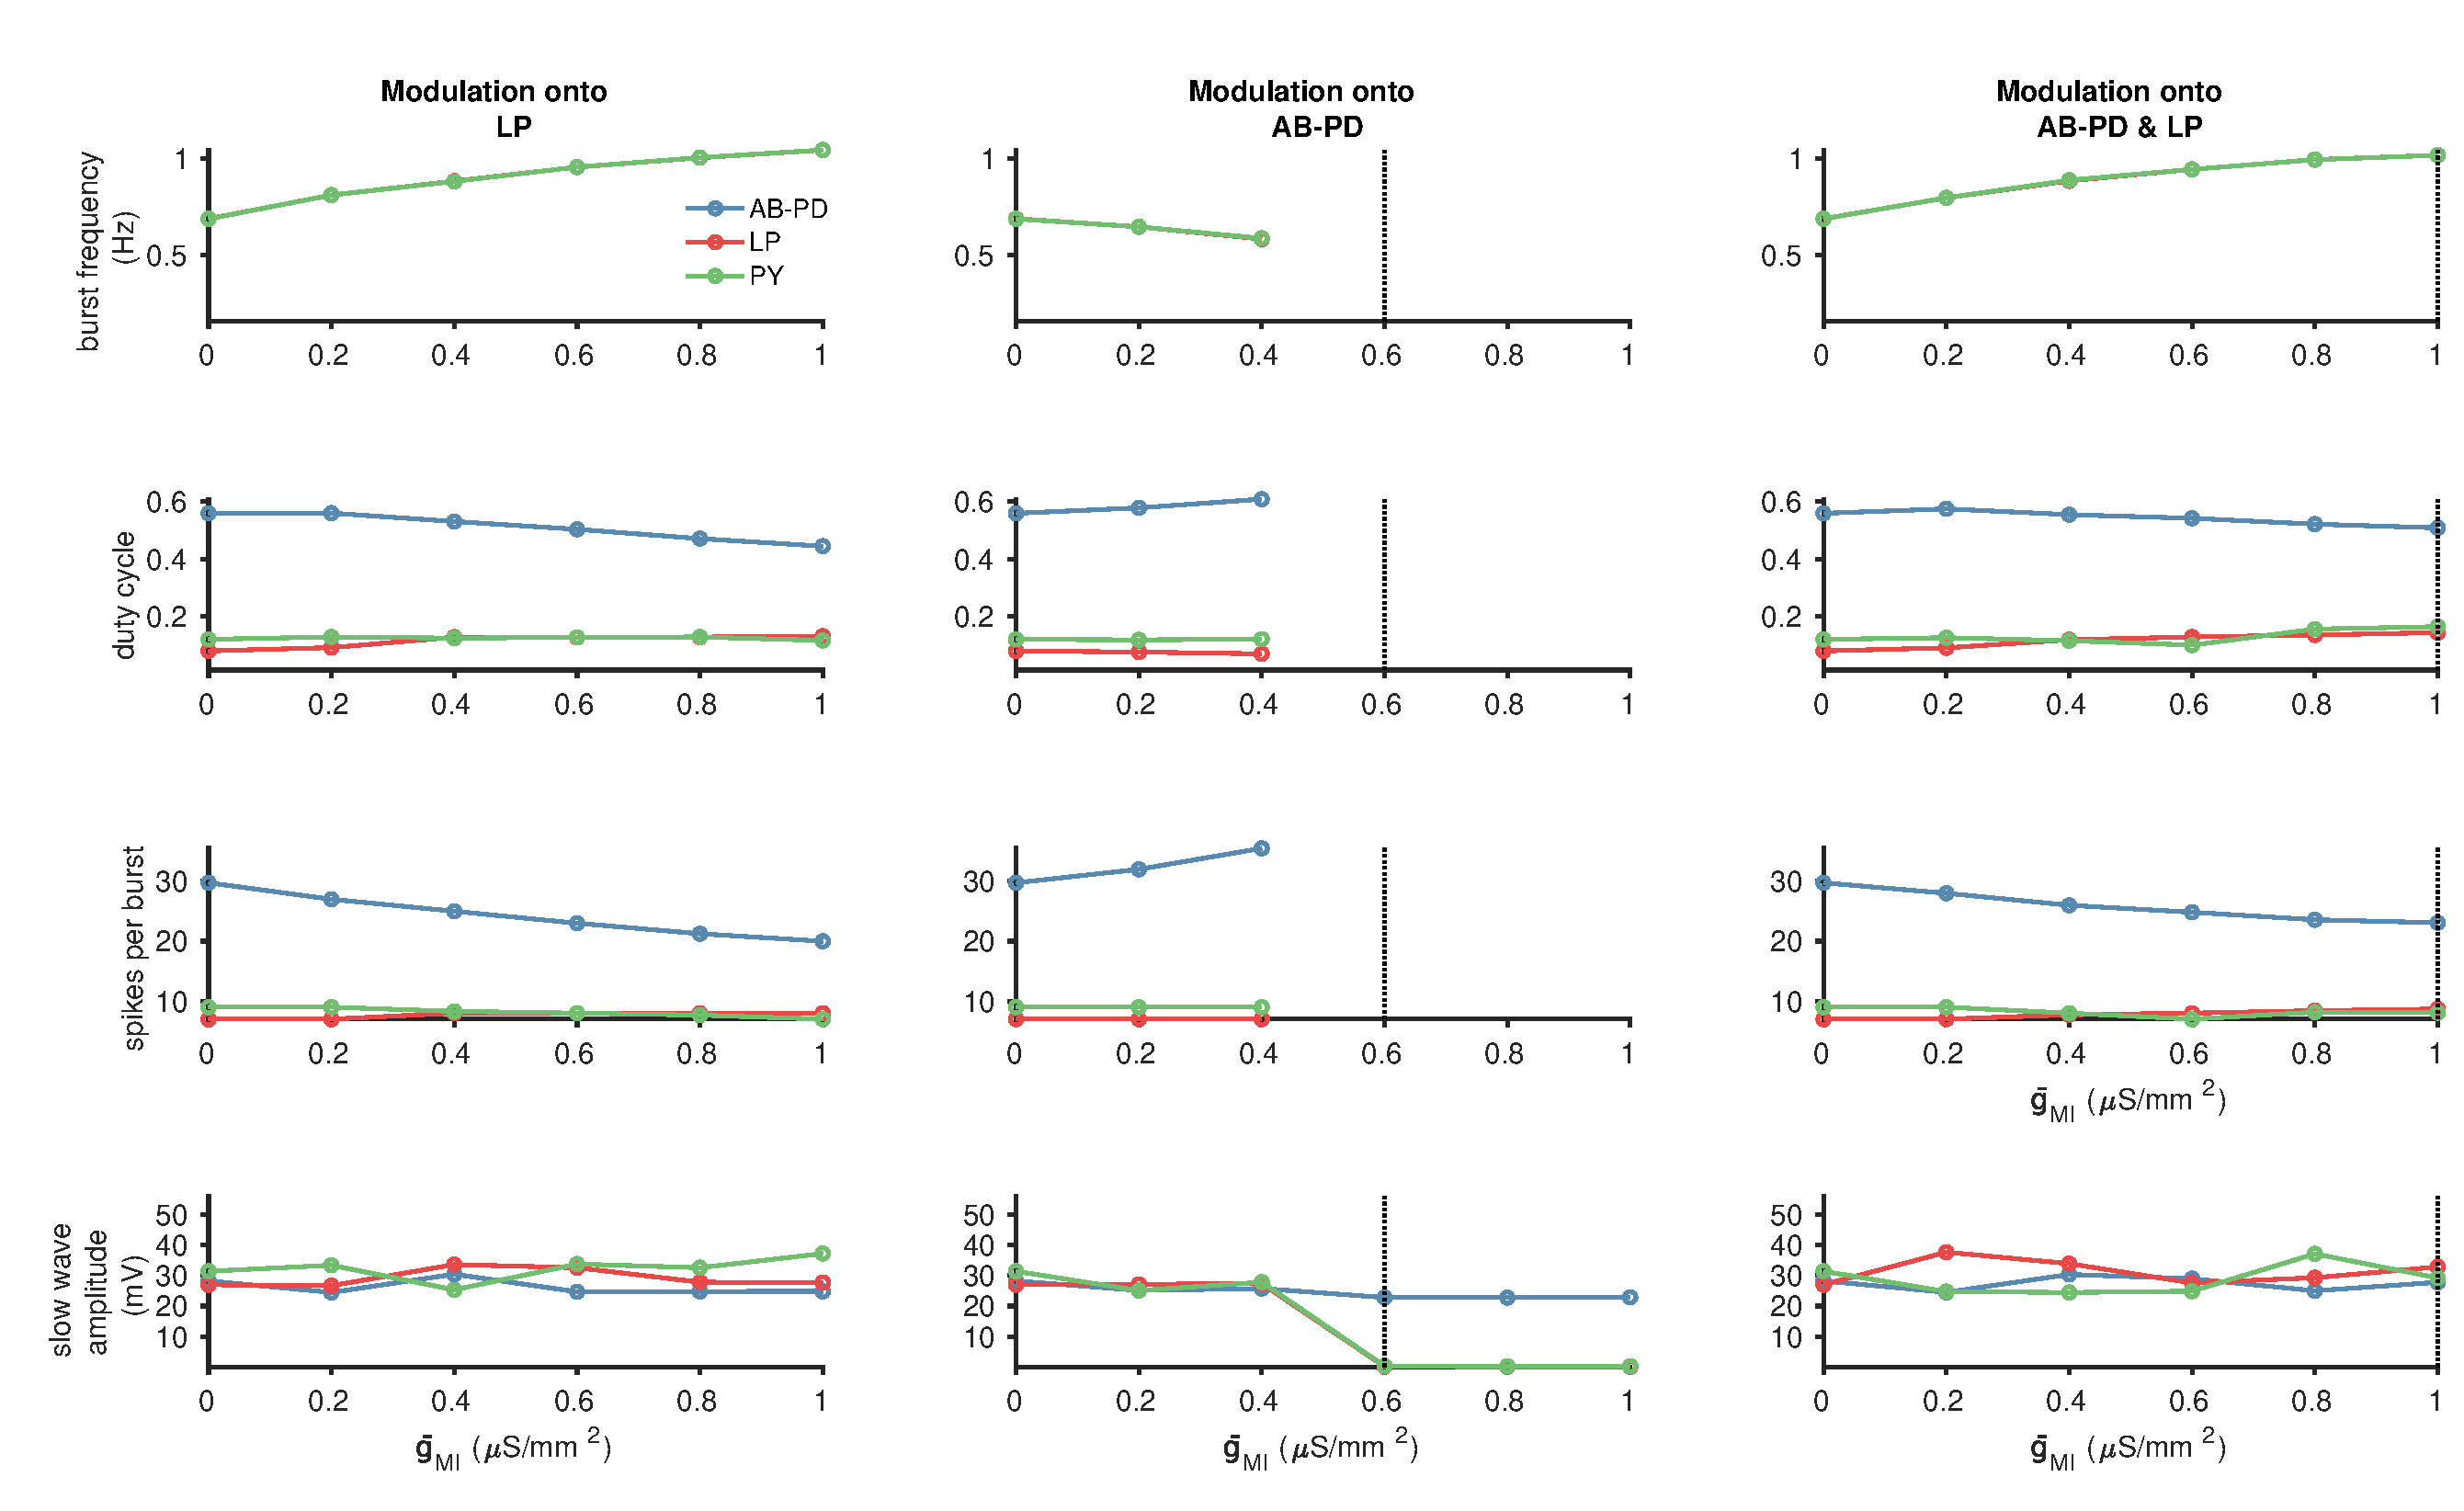
\includegraphics[width=1.0\linewidth]{gfx/all-modulation/metrics4}
	\caption[Modulation of AB-PD can elecit tonic spiking (metrics)]{Neuromodulation of the pacemaker model can result in tonic spiking. Modulation of LP offsets this effect, resulting in triphasic activity with increased frequency and amplitude with respect to the decentralized condition.}
	\label{fig:metrics4}
\end{figure}


%*****************************************
%*****************************************
%*****************************************
%*****************************************
%*****************************************
